\documentclass[electronic]{kthesis}

\usepackage[english]{babel}
\usepackage{import}
\usepackage{enumitem}

% copyright sign
\usepackage{textcomp}
\renewcommand{\copyright}{\textsuperscript{\textcopyright}}
\newcommand{\trademark}{\textsuperscript{\texttrademark}}

%% MATH
\usepackage{amsmath, amsfonts, amsthm}
\usepackage{nicefrac}
\usepackage{breqn}
\usepackage{tabularx}
\usepackage{stmaryrd} % for llbracket and rrbracket
\usepackage[ruled]{algorithm2e}

% LTL temporal operator
\DeclareFontFamily{U}{matha}{\hyphenchar\font45}
\DeclareFontShape{U}{matha}{m}{n}{
      <5> <6> <7> <8> <9> <10> gen * matha
      <10.95> matha10 <12> <14.4> <17.28> <20.74> <24.88> matha12
      }{}
\DeclareSymbolFont{matha}{U}{matha}{m}{n}
\DeclareMathSymbol{\vDash}{3}{matha}{'52}
\DeclareMathSymbol{\nvDash}{3}{matha}{'50}

\DeclareMathOperator*{\argmin}{arg\,min}
\makeatletter
\newcommand{\tuple}[1]{
	\@tempcnta=0
	\def\mylist{#1}
	\@for\next:=\mylist\do{
	\ifnum \@tempcnta = 0 \else ,\linebreak[1]\fi \next
	\advance\@tempcnta\@ne}
}
\makeatother

%\renewcommand{\splitatcommas}[1]{#1}

\newcommand{\buchi}[0]{B\"uchi}

%% LTL symbols defintion
\usepackage{latexsym} % get the right \Diamond symbol
\newcommand{\LTLalways}		{\ensuremath{\square}}
\newcommand{\LTLeventually}	{\ensuremath{\Diamond}}
\newcommand{\LTLuntil}		{\ensuremath{\mathsf{U}}}
\newcommand{\LTLnext}		{\ensuremath{\bigcirc}}
\newcommand{\LTLimply}			{\ensuremath{\rightarrow}}
\newcommand{\true}			{\ensuremath{\top}}


\newcommand{\outpost}{ \ensuremath{\overline{Post} } }
\newcommand{\inpre}{ \ensuremath{\overline{Pre} } }

%% MATH COMMANDS
\newcommand{\vect}[1]{\ensuremath{ \mathbf{#1}}}
\newcommand{\leftint}{\left \llbracket}
\newcommand{\rightint}{\right \rrbracket}
\newcommand{\abs}[1]{\left|#1\right|}
\newcommand{\card}[1]{\left|#1\right|}

%% GRAPHICS
\usepackage{graphicx}
\graphicspath{{./plots/}{./env/}{./results/}}
\usepackage[mode=buildnew]{standalone}
\usepackage{epstopdf}

\usepackage{tikz}
\usetikzlibrary{shapes.geometric, arrows, positioning, calc, fit, arrows, decorations.pathreplacing}
\usepackage{pgfplots}
\usepgfplotslibrary{groupplots}

% DEFINITION/THEOREM ENVIRONMENTS
\newcommand{\inlinedef}[1]{\textit{#1}}

\newtheorem{theorem}{Theorem}
\newtheorem{problem}{Problem}
\newtheorem{olddefinition}{Definition}
\newtheorem{property}{Property}
\newtheoremstyle{named}{}{}{\itshape}{}{\bfseries}{.}{.5em}{#1 \thmnumber{#2} \thmnote{(#3)}}
\theoremstyle{named}
\newtheorem{namedtheorem}[theorem]{Theorem}
\newtheorem{nameddefinition}[olddefinition]{Definition}
\newtheorem{namedproperty}[property]{Property}

\newcommand{\thmsymbol}{\( \blacktriangle \)}
\newcommand{\propsymbol}{\( \blacklozenge \)}

\newenvironment{nameddef}[1]
    {\begin{samepage}
    \begin{nameddefinition}[#1]
    \renewcommand{\qedsymbol}{\thmsymbol}\pushQED{\qed}
    }
    {
    \popQED % in order to pop it before (in case of itemize) just call it in an item
    \end{nameddefinition} 
    \end{samepage}
    }
\newenvironment{namedprop}[1]
    {\begin{samepage}
    \begin{namedproperty}[#1]
    \renewcommand{\qedsymbol}{\propsymbol}\pushQED{\qed}
    }
    {
    \popQED % in order to pop it before (in case of itemize) just call it in an item
    \end{namedproperty} 
    \end{samepage}
    }
\newenvironment{namedtheo}[1]
    {\begin{samepage}
    \begin{namedtheorem}[#1]
    \renewcommand{\qedsymbol}{\propsymbol}\pushQED{\qed}
    }
    {
    \popQED % in order to pop it before (in case of itemize) just call it in an item
    \end{namedtheorem} 
    \end{samepage}
    }
\newenvironment{prop}[0]
    {\begin{samepage}
    \begin{property}
    \renewcommand{\qedsymbol}{\propsymbol}\pushQED{\qed}
    }
    {
    \popQED % in order to pop it before (in case of itemize) just call it in an item
    \end{property} 
    \end{samepage}
    }
\newenvironment{definition}[0]
    {\begin{samepage}
    \begin{olddefinition}
    \renewcommand{\qedsymbol}{\thmsymbol}\pushQED{\qed}
    }
    {
    \popQED % in order to pop it before (in case of itemize) just call it in an item
    \end{olddefinition} 
    \end{samepage}
    }
    
    
%% TRANSITION SYSTEM COMMANDS
\usepackage[all]{xy}
\usepackage{amssymb}
\newdir{|>}{-{\scriptscriptstyle{\blacktriangleright}}}
\newcommand{\transition}{
  \ensuremath{ \xymatrix{\ar@{-|>}[r]&} }
  }
\newcommand{\labelledtransition}[1]{
  \ensuremath{ \xymatrix{\ar@{-|>}[r]^{#1}&} }
  }
\newcommand{\systransition}[2]{
  \ensuremath{ \xymatrix{\ar@{-|>}[r]^{#2}_{#1}&} }
  }

\newcommand{\Post}[2]{Post_{#2}^{#1}}
\newcommand{\Reach}[2]{Reach^{#1}({#2})}
\newcommand{\ReachSeq}[2]{Reach^{*#1}(#2)}

\newcommand{\sysDef}[1]{(\)}
  
%% COMMENTS
\usepackage{color}
\definecolor{colorcomment}{RGB}{100,0,250}
\renewcommand{\comment}[1]{\textit{\textbf{\color{colorcomment} #1}}}

%% SUPER SCRIPT STUFF
\makeatletter
\newcommand\newsubcommand[3]{\newcommand#1{#2\sc@sub{#3}}}
\def\sc@sub#1{\def\sc@thesub{#1}\@ifnextchar_{\sc@mergesubs}{_{\sc@thesub}}}
\def\sc@mergesubs_#1{_{\sc@thesub#1}}

\newcommand\newsupcommand[3]{\newcommand#1{#2\sc@sup{#3}}}
\def\sc@sup#1{\def\sc@thesup{#1}\@ifnextchar^{\sc@mergesups}{^{\sc@thesup}}}
\def\sc@mergesups^#1{^{\sc@thesup#1}}
\makeatother

\newcommand{\T}[1]{#1{}^\top}
\newcommand{\proj}[1]{|_{#1}}

\renewcommand{\exp}[1]{e^{#1}}

\begin{document}



\title{Abstraction reduction and multi agent control with Linear Temporal Logic specifications}
\subtitle{A non deterministic approach}
\author{Paul Rousse}
\date{Today}
\thesistype{Master of Science Thesis}
\imprint{}
\disputationsdatum{}
\disputationslokal{}
\publisher{}
\examen{}

\frontmatter

\maketitle

\mainmatter 

\newcommand{\SSunobs}{\mathfrak{X}^i}
\newcommand{\SSobs}{\mathfrak{X}^o}
\newcommand{\Ninputs}{\Delta n_u}%
\newcommand{\y}{\vect{y}}%
\newcommand{\x}{\vect{x}}%
\newcommand{\xa}{\vect{x}^a}%
\newcommand{\xobs}{\vect{x}^o}%
\newcommand{\Xobs}{X^o}%
\newcommand{\Xobsinit}{X^o_0}%
\newcommand{\xunobs}{\vect{x}^i}%
\newcommand{\Xunobs}{X^i}%
\newcommand{\Sunobs}{\mathcal{S}^i}%
\newcommand{\Xuinv}{{\mathcal{X}^i}}%
\newcommand{\pastuseq}{\vect{u}_{n-\Ninputs},\dots,\vect{u}_{n-1}}%
\newcommand{\pastuseqn}{\vect{u}_{n+1-\Ninputs},\dots,\vect{u}_{n}}%
\newcommand{\Pastuseq}{U_n}%
\newcommand{\sys}{\mathcal{S}}%
\newcommand{\sysa}{\mathcal{S}_a}%
\newcommand{\sysaU}{\mathcal{U}}%
\newcommand{\sysA}{\mathcal{S}_A}%
\newcommand{\sysB}{\mathcal{S}_B}%
\newcommand{\Usys}{\mathcal{U}}%
\newcommand{\Wsys}{\mathcal{W}}%
\newcommand{\Uunobs}{{\mathcal{U}^i}}%
\newcommand{\Wunobs}{{\mathcal{W}^i}}%
\newcommand{\uobs}{\vect{u}^o}%
\newcommand{\wobs}{\vect{w}^o}%
\newcommand{\uunobs}{\vect{u}^i}%
\newcommand{\wunobs}{\vect{w}^i}%
\newcommand{\Dunobs}{n^i}% Dimension of the ss of unobs
\newcommand{\R}{\mathbb{R}}% real set
%%
% Monotone systems
\newcommand{\mle}{\prec}
\newcommand{\mleq}{\preceq}
\newcommand{\minf}[1]{\underline{#1}}
\newcommand{\msup}[1]{\overline{#1}}
%%
% linear system
\newcommand{\X}{X}%
\newcommand{\Xinv}{\mathcal{X}}%
\newcommand{\U}{\mathcal{U}}%
\newcommand{\W}{\mathcal{W}}%
\newcommand{\vu}{\vect{u}}%
\renewcommand{\u}{\vect{u}}%
\renewcommand{\U}{\mathcal{U}}%
\newcommand{\w}{\vect{w}}%
\newcommand{\s}{\vect{s}}%
\newcommand{\st}{\vect{t}}%
%
% Continuous model
\newcommand{\traj}{\varphi}
%
% discretization of the abstraction
\newcommand{\xd}{\x_d}
\newcommand{\vd}{\vect{v}_d}
\newcommand{\Nobs}{N^o} % number of states of the discretization of the state space \SSobs
%
\section{Introduction}

\comment{
One of the justification of my model is that we can accept some noise and still find a controller. In my case, I have been using a really simple controller. But in a real case scenario, it would be better to use pwa controller that produce smoother trajectories.
}

\comment{
Despite the fact that we have self loops, we keep the timing information by using some computation of the average control.
}


\chapter{Abstraction reduction}
\newcommand{\Cont}{\mathcal{C}}%
%
% Introduction of the necessity of reduction of an abstraction
Graph search algorithm complexities are dependant on the size of the abstraction.
These methods suffer from the state space explosion problem: the complexity of graph search algorithm have usually an exponential complexity in the size of the state space.

% Property that needs to be verified by the abstraction
Therefore it is of a great interest to design small abstractions for the controller synthesis.
The new abstraction needs to verify alternating similarity relationship with the original abstraction.

The term "reduction" will be justified later. But this does not always correspond to a reduction of the abstraction size (the set of all the input sequences might be larger than the size of the states dimensions that have be suppressed). However, the efficient utilizations of this method will correspond to a reduction of the state space size.

\section{Related work}
Talk about formal verifications methods.

The needs of discrete abstraction.

%% MOVE THIS PART
In \cite{tabuada2009verification}, the link between in hybrid systems is investigated. 
\begin{nameddef}{System}\label{def:system}
$S = (X,X_0,\U, \systransition{S}{}, Y,H)$
where:
\begin{itemize}[noitemsep,nolistsep]
\item $X$ is a set of states;
\item $X_0 \subset X$ a set of initial states;
\item $\U$ a set of inputs;
\item $\systransition{S}{} \subseteq X \times \U \times X$ a transition relation ;
\item $Y$ a set of outputs;
\item $H:X \rightarrow Y$ an output map.\popQED
\end{itemize}
\end{nameddef}

Note: in the future we will use a second equivalent notations for the transition relation $\systransition{S}{\u}$ of a system $S$: $\Post{S}{\u}$  defined for $\x \in X$ and $\u \in \U$ by:
\begin{equation}
\Post{S}{\u}(\x) = \{ \x \in X \mid \exists \x' \in X, \x \systransition{S}{\u} \x' \}
\end{equation}

\comment{This system can model both discrete and continuous systems, which make it a good candidate in order to deal with hybrid systems.}

The alternating simulation relation between 2 systems is the link between discrete abstraction and the continuous representation of this system.
For comoditiy, the definition of alternative simulation is rewritten here (\cite{tabuada2009verification}):
\begin{nameddef}{Alternating simulation} \label{def_alt_sim}
Let $\sysA$ and $\sysB$ 2 systems with $Y_a=Y_b$, $\sysA$ is alternatingly simulated by $\sysB$ if there exists a relation $R \subseteq X_a \times X_b$ that verify:
\begin{enumerate}[noitemsep,nolistsep]
\item $\forall x_{a0} \in X_{a0}, \exists x_{b0} \in X_{b0}, (x_{a0},x_{b0}) \in R$
\item $\forall (x_a,x_b) \in R, H_a(x_a) = H_b(x_b)$
\item $\forall (x_a,x_b) \in R, \forall u_{a} \in \U_{a}, \exists u_{b} \in \U_{b}$\\
$\forall x_b' \in \Post{\sysB}{u_b}(x_b),\exists x_a' \in \Post{\sysA}{u_a}(x_a), (x_a',x_b') \in R$
\popQED
\end{enumerate}
\end{nameddef}
The alternating simulation relation between $\sysA$ and $\sysB$ is weaker than the bisimulation relation (that require the alternating simulation relation between $\sysA$ and $\sysB$ and between $\sysB$ and $\sysA$).

Lets denote the composition of systems by the operator $\times$.
If $\sysA$ alternatingly simulate by $\sysB$ for a controller $\Cont$ composable with $\sysA$ or $\sysB$, then $\sysA \times \Cont$ verify the same reachability properties than $\sysB \times \Cont$, and $\sysB \times \Cont$ verify the same safety properties than $\sysA \times \Cont$.


%% INPUT SEQUENCE REACHABLE SETS
In the next part we will focus on systems with inputs memory. The knowledge of unobserved variables will be replaced by the knowledge of an input sequence $\Pastuseq$.

For a system $S$, let $\Reach{S}{U} \subseteq X$ defined for a finite sequence $U \in \U^\star$ of $N \in \mathbb{N}$ control actions by:
\begin{equation}
\begin{split}
\x \in \Reach{S}{U}
\Leftrightarrow &
\exists \x_0 \in X_0,
\forall i<N, \exists \x_i \in X,\\
&\x_0 \systransition{S}{\u_0} \x_1
\systransition{S}{\u_1} \dots
\systransition{S}{\u_{N-1}} \x
\end{split}
\end{equation}
$\Reach{S}{U}$ correspond to all the reachable states with the sequence inputs $U$.

%% Define the reached states:
\renewcommand{\v}{\vect{v}}
\newcommand{\useq}{\v_{1-n},\dots,\v_{0}}
\begin{definition}
For a finite sequence $\Pastuseq = \left\{ \useq \right\}$ of $n$ controls in $\U$,
let $X(\Pastuseq) \subseteq X$ the set of all the states reached by a control sequence terminating with $\Pastuseq$:
\begin{equation}
\ReachSeq{S}{\Pastuseq}
=
\bigcup_{\{\vu_i\}_{i \le \infty} \in \U^\star}
\Reach{S}{\{\vu_0,\vu_1,\dots,\useq\}}
\end{equation}
\end{definition}

\section{Introduction}
We will first introduce the abstraction used, then treat the case of dynamical systems, then with linear systems.


\section{Abstraction reduction} \label{sec:abstraction}
\comment{Questions: Which system to choose and when? Idea, I begin with the definition of the system to introduce the reached sets, give the property of alterning simulation relation for this type of system and then go for dynamical systems, talk about the reached sets.}%
\comment{Define the reached sets.}%
\comment{Do I want to talk about an abstraction or a system?}%
\comment{How can it reduce the size if it is a continuous system?}%
\comment{Partir d'un system discret}%
%
\comment{I need to create the abstraction with memories first.}%
%
Let the system $\sys = (\tuple{X,X_0,\U,\transition,Y,H})$
and the same system extended with a memory of the last $\Ninputs$ control actions $\sys'$ defined by
$\sys' =  (\tuple{X',X_{0}',\U,\transition,Y',H'})$ 
where:
\begin{itemize}[nolistsep,noitemsep]
\item $X' = X \times \U^{\Ninputs}$ the set of states, 
\item $X_{0}' = X_0 \times \U^{\Ninputs}$ the set of initial states,
\item $Y' = Y \times \U^{\Ninputs}$ the set of outputs,
\item $H'$ the output map defined for all $(x,\Pastuseq) \in X'$ as $H'(x') = (H(x),\Pastuseq)$
\item and the transition relation defined by:
\begin{equation}
\begin{split}
(\x,\u_{n - \Ninputs},...,\u_{n-1}) 
\systransition{S'}{\u} &
 (\x',\u_{n+1-\Ninputs},...,\u_{n-1},\u)\\
\Longleftrightarrow 
&
\left\{
\begin{split}
&\x \systransition{S}{\u} \x' \\
&\x \in \ReachSeq{S}{\u_{n - \Ninputs},...,\u_{n-1}}
\end{split}
\right.
\end{split}
\end{equation}
\end{itemize}

In this section we will design an abstraction $\sysa$ that alternately simulate the system $\sys'$.

% Describe how it is done
In control synthesis we would use abstraction in order to design a controller that will be used afterward by the original system. If the system and its abstraction verify a property of bisimulation, then all the property of the abstraction composed with the controller hold for the original system composed with the same controller. In other words, the bisimulation relation guaranty that reachability and safety properties are the same.
However, most of the time this relation is too demanding.
In our case, we will just guaranty the alternating simulation relation between $\sys$ and $\sysa$ which conserve the reachability properties between 2 systems.
\comment{Talk with Pierre Jean about this part.}

We will assume that the state $\x$ of the system $\sys$ can be decomposed in this way $\displaystyle\T{\x} = \T{[\T{\xobs},\T{\xunobs}]}$ where $\xobs \in Y$ can be observed and $\xunobs$ is an unobserved (internal) state.
Lets call $\SSunobs$ the subspace of $\xunobs$ and $\SSobs$ the one of $\xobs$.
The states of the reduced abstraction $\sysa$ will be expressed by $\xa_n = [\xobs_n,\Pastuseq]$ where $\Pastuseq = [\pastuseq]$ correspond to the $\Ninputs$ last control actions.


Lets define the set $\Xunobs(\Pastuseq) = \Reach{S}{\Pastuseq} \proj{\SSunobs}$
Literally, $\Xunobs(\Pastuseq)$ correspond to all the states that can be reached with control sequences terminating with $\Pastuseq$.
We can now "replace" the knowledge of the state  $\xunobs$ by the set of all the possible states $\Xunobs(\Pastuseq)$ after applying $\Pastuseq$.
% Definition of the reduced system
Let the system
$\sysa =  (X_a,X_{a 0}, \sysaU, \transition, Y_a, H_a)$ 
where:
\begin{itemize}[nolistsep,noitemsep]
\item $X_a = \Xobs \times \sysaU^{\Ninputs}$ the set of states, 
\item $X_{a 0} = \Xobsinit \times  \mathcal{U}^{\Ninputs}$ the set of initial states,
\item $Y_a = \Xobs \times \U^\Ninputs$ the set of outputs,
\item $H_a$ the output map that correspond to the projection from $X_a$ on $\Xobs$.
\item and the transition relation is defined by:
\begin{equation}
\begin{split}
(\xobs_n,\vect{u}_{n - \Ninputs},...,\vect{u}_{n-1}) 
\labelledtransition{\vu} 
& (\xobs_{n+1},\vect{u}_{n+1-\Ninputs},...,\vect{u}_{n-1},\vu)\\ \Longleftrightarrow 
\xobs_{n+1} \in 
& H_a(Post^S_{\vu}(\{\xobs\} \times \Xunobs(\vect{u}_{n - \Ninputs},...,\vect{u}_{n-1}))
\end{split}
\end{equation}
\end{itemize}

%% MISSING PROOF THAT IT IS AN ALTERNATING SIMULATION RELATION
\begin{prop}
\comment{I have been messing with the alternate simulation relation, I need to inverse all of them}
$\sysa$ is alternatingly simulated by $\sys'$.
\end{prop}

\begin{proof}
Let $R$ the relation defined by:
\begin{equation}
R = \{ (\x',\xa) \in X' \times X_a \mid H'(\x') = H_a(\xa) \}
\end{equation}
By definition of the systems $S'$, $\sysa$ and of the relation $R$, conditions 1 and 2 of definition \ref{def_alt_sim} are already verified.

In order to prove that condition 3 lie, it is sufficient to show that the unobserved part of $\x$ is contained in the set $\Xunobs(\Pastuseq)$.
As we know that for a all $\xunobs$,$ \xunobs \in \Xunobs(\Pastuseq)$, this imply that there ...

Let $(\x',\xa) \in R$, $\u \in U$ and $\x'_+ \in \Post{S'}{\u}(\x')$.
As $H'(\x') = H_a(\xa)$, $\x' \proj{\U^\Ninputs} = \xa \proj{\U^\Ninputs}$, we will denote this quantity with $\Pastuseq$.
By definition of $\Xunobs(\Pastuseq)$,
we know that $\x' \proj{\SSunobs} \in \Xunobs(\Pastuseq)$,
so
$\x' \in \{\x' \proj{\SSobs} \} \times \Xunobs(\Pastuseq) \times \Pastuseq$
which imply that
$\x'_+ \in \Post{S'}{\u}(\{\x' \proj{\SSobs} \} \times \Xunobs(\Pastuseq) \times \Pastuseq )$.
By taking $\xa_+ = H_a(\x'_+) \in \Post{S_a}{\u}(\xa)$,
we have $(\x'_+,\xa_+) \in R$.
\end{proof}

\section{Dynamical systems}
\comment{Add the dynamical representation of the system def.}

As the definition \ref{def:system} of a system can be used in order to represent continuous and discrete dynamical systems.
In this case, the computation of the sets $\Xunobs(\Pastuseq)$ is a reachability problem.
It can be solved in 2 steps: find the smallest invariant $\Xuinv$ of $\sys$ dynamics on $\xunobs$; compute $\Xunobs(\Pastuseq)$ the image of $\Xuinv$ after applying a control sequence that terminate with $\Pastuseq$.

\begin{figure}
\centering
%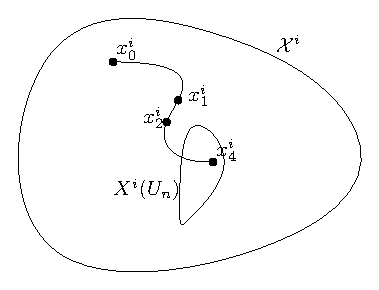
\includegraphics[width=0.5\linewidth]{invariant_set}
\caption{The image of the invariant set $\Xuinv$ after applying the control sequence $\Pastuseq$ is $\Xunobs(\Pastuseq)$}
\end{figure}

% Here I am trying to explain why I have been choosing a smaller class of systems
Interesting case scenarios happen when the knowledge about $\Xunobs(\Pastuseq)$ is preferable to the actual measure of the state $\xunobs$.
If $\Xunobs(\Pastuseq)$ is unbounded it can results in smaller abstraction (it can possibly create an infinite number of successors).
We will therefore focus on systems that have bounded invariant sets $\Xuinv$.

From now we will use linear time invariant systems. We use them mainly for their ease of manipulation.
\newcommand{\xinf}{\underline{\vect{x}}}%
\newcommand{\xsup}{\overline{\vect{x}}}%
\newcommand{\xinit}{\vect{x}_0}%
\newcommand{\traj}{\varphi}%
\newcommand{\xn}{\vect{x}_n}%
\newcommand{\un}{\vect{u}_n}%
\newcommand{\wn}{\vect{w}_n}%
\newcommand{\yn}{\vect{y}_n}%
\newcommand{\xnn}{\vect{x}_{n+1}}%
%
\section{Reached sets computation}
%
The computation of the reached sets is a field in control theory on its own.
So the reader might refer to the large literature about this field for more precise algorithms in order to find invariants and the reached sets.

In this part, we will present 2 methods to compute the reached sets.
The first one will only be valid for monotone systems, even if this class is restrictive, it is possible to obtain a closed form solution for the problem which might be useful for further studies.
The second one is based on ellipsoidal bounding methods which can be applied to a wider class of systems. 


\subsection{Monotone systems}
Monotone systems are systems that keep a partial ordering relation between 2 trajectories. With this property, we can bound a set by 2 vectors $\xinf$ and $\xsup$.
For all the trajectories starting at $\xinit \in [\xinf,\xsup]$, we know that
\begin{equation}
\forall k \in \mathbb{N}, \traj(\xinit,k) \in [\traj(\xinf,k),\traj(\xsup,k)]
\end{equation}

We will work with a linear monotone system defined by:
\begin{equation} \label{sys:monotone_lti}
\begin{split}
\xnn &= A \xn + B \un + E \wn \\
\yn &= C \xn
\end{split}
\end{equation}

\cite{liu2014abstraction} have been investigating boundedness property in order ignore one part of the abstraction.
Really good introduction about hierarchical control approach, give references.

Let define the system $S$

\begin{align*}
\mathbf{x}_{n+1} &= 
\begin{bmatrix} A_z & A_{zr}\\ 0 & A_r \end{bmatrix} \mathbf{x}
+\begin{bmatrix} B_z \\ B_r \end{bmatrix} \mathbf{u}
+\begin{bmatrix} E_z\\ E_r \end{bmatrix}\mathbf{w}\\
\mathbf{y}_n &= \mathbf{x}^z_n
\end{align*}
with,
\begin{align*}
\mathbf{x}_n = \begin{bmatrix}
\mathbf{x}^z_n\\
\mathbf{x}^r_n
\end{bmatrix}
\textrm{, }
\mathbf{u} = \begin{bmatrix}
\mathbf{u}^z_n\\
\mathbf{u}^r_n
\end{bmatrix}
\textrm{, }
\mathbf{w}_n = \begin{bmatrix}
\mathbf{w}^z_n\\
\mathbf{w}^r_n
\end{bmatrix}
\end{align*}

Let $S_r=(A_r,B_r,E_r)$ the subsystem of $S$, $\mathcal{U}_r$ and $\mathcal{W}_r$ the projection of $\mathcal{U}$ and $\mathcal{W}$ on the reduced system input space and noise space respectively.

We will assume the subsystem $S_r$ is a monotone stable system and that the inputs and noise are bounded.
These hypotheses might seems really restrictive, however most of the control strategy consist of stabilizing one part of the system that might be independent of the rest of the system.
Further analysis will show that if the controlled part of the system is as reactive as the abstraction sampling time, this reduction might lead to good results.

We would like to find all the reachable states of $S_r$.
Let $|\lambda_1| \leq ... \leq |\lambda_{n_r}|$ the eigenvalues of $A_r$, as the system $S_r$ is asymptotically stable $|\lambda_{n_r}|<1$,
so the eigenvalues of the matrix $I-A_r$ are all greater than 0.
Let define:
\begin{equation}
\begin{split}
\overline{\mathbf{x}}^r &= (I-A_r)^{-1} (B_r \overline{\mathbf{u}}^r + E_r \overline{\mathbf{w}}^r)\\
\underline{\mathbf{x}}^r &= (I-A_r)^{-1} (B_r \underline{\mathbf{u}}^r + E_r \underline{\mathbf{w}}^r)\\
\end{split}
\end{equation}

where $\mathcal{U}^r \subset \left [\underline{\mathbf{u}}^r, \overline{\mathbf{u}}^r \right ]$ and $\mathcal{W}^r \subset \left [\underline{\mathbf{w}}^r, \overline{\mathbf{w}}^r \right ]$, such bounds exists as we assumed that $\mathcal{U}_r$ and $\mathcal{W}_r$ are bounded.

Let $\varphi_r (\mathbf{x}^r,U_r,W_r)$ the trajectory function of the system $S_r$ starting from $\mathbf{x}^r$
applying the control sequence $U_r \in \mathcal{U}_r^\star$
with the noise sequence $W_r \in \mathcal{W}_r^\star$.
As the system $S_r$ is monotone,
$$
\forall \mathbf{x}^r \in \left [\underline{\mathbf{x}}^r, \overline{\mathbf{x}}^r \right ],
\forall U_r \in \mathcal{U}_r^\star,
\forall W_r \in \mathcal{W}_r^\star,
\varphi_r(\mathbf{x}^r,U_r^e,W_r)
\in \left [\underline{\mathbf{x}}^r, \overline{\mathbf{x}}^r \right ]$$

If the initial state of the reduced system is in $\left [\underline{\mathbf{x}}^r, \overline{\mathbf{x}}^r \right ]$, then every trajectories will stay in this set.

For $U_r \in \mathcal{U}_r^\star$, let $X_r(U_r)$ the subset of $\mathbb{R}^r$ defined by:
\begin{equation}
X_r(U_r) = \left [ 
\varphi_r(\underline{\mathbf{x}}^r,U_r,\underline{\mathbf{w}}^r),
\varphi_r(\overline{\mathbf{x}}^r,U_r,\overline{\mathbf{w}}^r)
\right ]
\end{equation}
$X_r(U_r)$ correspond to the set of all the possible successors after applying the control sequence $U_r$ on the system $S_r$. This results come from the monotonic property.
This can be summarized in the following property:
$$
\forall U_r \in \mathcal{U}_r^\star,
\forall \mathbf{x}^r \in \left [\underline{\mathbf{x}}^r, \overline{\mathbf{x}}^r \right ],
\forall W_r \in \mathcal{W}_r^\star,
\varphi_r(\mathbf{x}^r,U_r,W_r)
\in X(U_r)$$

\subsection{Extension to non monotonic systems}
The main argument behind the reduction is the ability to bound the dynamic in a set and to work with these boundaries (which are easier to manipulate than a complete system).
The monotonicity property is really convenient in order to perform the computations.
However, this is a strong assumption on the system that cannot be met in every situations: any system that have a non real eigenvalues is not monotonic.
In this part we will have a Lyapunov approach for a linear system.
The Lyapunov function will not be used to proof the stability of the system but to perform operations on bounding sets of our dynamic.

The natural representation of bounds with the monotonicity property are rectangle, in our case, the lyapunov function that we will use is a quadratic function $\vect{x}^T P \vect{x}$ where $P$ is a definite positive matrix.
Even if the lyapunov approach is usable for a monotonic, we will see that it is less efficient than the monotonic approach.

To perform the reduction, we have to find the best combination of applying the reduction: the different theory must be used in a proper way. The monotonicity property depends on the base of the system. The lyapunov function efficiency also depend on the frame.

Lets consider the previous linear system.
Lets denote $x^\star(u,w)$ the equilibrium point of the linear system, the previous assumptions about global stability will still hold:
\begin{equation}
\vect{x}^\star(\vect{u},\vect{w}) = A^{-1} (B \vect{u} + E \vect{w})
\end{equation}

\begin{equation}
\vect{x}^{\star}_{\vect{u}} = \vect{x}^\star(\vect{u},\vect{0})
\end{equation}

Lets define the following Lyapunov function obtained by solving the Lyapunov equation $A^T P + P A = -Q$ where $Q$ and $P$ are positive definite ($Q$ is given):

\newcommand{\xu}{\vect{x}^{\star}_{\vect{u}}}
\newcommand{\Vu}{V_{\vect{u}}}
\begin{equation}
\Vu(\vect{x}) = (\vect{x} - \xu) ^T P (\vect{x} - \xu) 
\end{equation}

In the next paragraphs, we will try to find invariant sets:
\begin{align*}
\dot{\Vu}(t) =& \dot{\vect{x}}^T(t) P (\vect{x}(t) - \xu) +  (\vect{x}(t) - \xu)^T P \dot{\vect{x}}(t)
\\
 =& (A \vect{x}(t) + B \vect{u} + E \vect{w}(t))^T P (\vect{x}(t) - \xu)\\
 & + (\vect{x}(t) - \xu)^T P (A \vect{x}(t) + B \vect{u} + E \vect{w}(t))
\\
 =& (A (\vect{x}(t) - \xu) + E \vect{w}(t))^T P (\vect{x}(t) - \xu)\\
 & +(\vect{x}(t) - \xu)^T P (A (\vect{x}(t) - \xu)+ E \vect{w}(t))
\\
 =& (\vect{x}(t) - \xu)^T A^T P (\vect{x}(t) - \xu) +  (\vect{x}(t) - \xu)^T P A (\vect{x}(t) - \xu)\\
 & + (E \vect{w}(t))^T P (\vect{x}(t) - \xu) +  (\vect{x}(t) - \xu)^T P E \vect{w}(t)
\\
 =& - (\vect{x}(t) - \xu)^T Q (\vect{x}(t) - \xu)\\
 & +\vect{w}(t)^T E^T P (\vect{x}(t) - \xu) +  (\vect{x}(t) - \xu)^T P E \vect{w}(t)\\
\end{align*}

Please note the following inequality:
\begin{equation}
- (\vect{x}(t) - \xu)^T Q (\vect{x}(t) - \xu) \leq - \alpha \Vu
\end{equation}

where
\begin{equation}
\alpha = \frac{\lambda_{min}(Q)}{\lambda_{max}(P)}
\end{equation}
Thanks to the positive definite property of $Q$ and $P$, we have $\alpha>0$.

In the next part we will try to find an upper bound for $(\vect{x}(t) - \xu)^T P E \vect{w}(t)$ and $(E \vect{w}(t))^T P (\vect{x}(t) - \xu)$.

We want to solve the following problem:
\begin{equation} \label{eq:max_w}
\max_{\vect{w} \in \mathcal{W}} \vect{b}^T \vect{w}
\end{equation}
In order to simplify the problem, we will take $\mathcal{W} = \{ \vect{w} \in \mathbb{R}^q \mid \vect{w}^T R \vect{w} \leq S\}$ where $R$ is a (strictly) positive definite matrix and $S>0$ a real number that correspond to the noise magnitude.
By writing the Lagrange multiplier, we can find that the maximum of this function is reached when:
\begin{equation}
\tilde{\vect{w}} = \frac{S^{\nicefrac{1}{2}} R^{-1} \vect{b}}{(\vect{b}^T R^{-1} \vect{b})^{\nicefrac{1}{2}}}
\end{equation}
\textit{Carefull there, it is not always defined!!!}

The maximum of $(\vect{x} - \xu)^T P E \vect{w}$ for a given $\vect{x}$ and $\xu$ is:
\newcommand{\Vwu}{V_{\vect{u}}^{\mathcal{W}}}
\textit{This result is false, it must be something like $P E^T R E P^T $}
\begin{equation}
\Vwu(\vect{x}) = [S (\vect{x} -\xu)^T E^T P R P^T E (\vect{x} -\xu)^T ]^{\nicefrac{1}{2}}
\end{equation}
\textit{I need to compute the actual value of $\beta$}
Let $K = E^T P R P^T E$
We will assume that $K$is defined positive.
This hypothesis is not too strong, $R$ has been chosen positive definite.
$P$ is already chosen to be positive definite.
So $E$ needs to be positive definite so that $K$ is positive definite.

For all $\vect{x} \in \mathcal{X}$, let $\vect{y} = \vect{x} -\xu$:
$$\vect{y}^T K \vect{y} \leq  \lambda_{max}(K) \vect{y}^T \vect{y}$$
As $P>0$, $\lambda_{min}(P)>0$:
$$\vect{y}^T \vect{y} \leq \frac{1}{\lambda_{min}(P)}  \vect{y}^T P \vect{y}$$
We have $\Vu(\vect{y}) = \vect{y}^T P \vect{y}$, so:
$$\vect{y}^T K \vect{y} \leq \frac{\lambda_{max}(K)}{\lambda_{min}(P)}  \Vu(\vect{y})$$
\newcommand{\Bu}{\beta}
We will define $\Bu$ by:
$$\Bu = 2\sqrt{S \frac{\lambda_{max}(K)}{\lambda_{min}(P)} }$$

\begin{equation}
\Vwu(\vect{x}) < \frac{\Bu}{2} [\Vu(\vect{x})]^{\nicefrac{1}{2}}
\end{equation}
where $\Bu$ is computed with eigenvalues of $E$, $P$, and $R$.

From now we have the following inequality:
\begin{equation}
\dot{\Vu}(t) \leq -\alpha \Vu(t) + \Bu \Vu^{\nicefrac{1}{2}}(t)
\end{equation}

Please note that this inequality is "optimal" in the sense that the upper boundary is reached when  we choose $\vect{w}$ solution of the maximization problem \ref{eq:max_w}.

\begin{prop} \label{ineq:lyap}
The function $\Vu$ verify this inequality for all $t',t \in \mathbb{R}^+$, with $t'>t$:
\begin{equation}
\Vu(t') \leq  \left[ (\sqrt{\Vu(t)} - \frac{\Bu}{\alpha}) e^{-\frac{\alpha}{2} (t'-t)} + \frac{\Bu}{\alpha} \right] ^2
\end{equation} 
\end{prop}

\begin{proof}
\newcommand{\tI}{\underline{I}}
\newcommand{\tIs}{\overline{I}}
\textit{Choose another name for $u$, $u$ must just be the system input.}
For a trajectory $\vect{x}(t)$, the function $\Vu(t)$ is a continuous piecewise differentiable function as it can be expressed as the integral of a piecewise continuous function.
So we will limit the proof to this class of functions.

Let $u$ a continuous piecewise differentiable function that verify:
\begin{align*}
\dot{u} &\leq -\alpha u + \beta u^{\nicefrac{1}{2}}\\
u & \geq 0
\end{align*}
Let $I$ an interval of $\mathbb{R}^+$ (possibly unbounded).
If $\forall t\in I, u(t)=0$, as $\beta,\alpha>0$ the property is proved.
Let $I^0$ the interior of $I$.
Lets choose $I$ so that u is strictly positive and differentiable on $I^0$.
Let $f$ a function defined in $I^0$ by $f = \sqrt{u}$.
We have:
$$\dot{f} = \frac{\dot{u}}{2\sqrt{u}}$$
using the inequality, we get (in $I^0$):
$$\dot{f} \leq -\frac{\alpha}{2} f + \frac{\beta}{2}$$
Let $g = f- \nicefrac{\beta}{\alpha}$ (defined on $I^0$), 
by definition of $f$, $g$ is continuous and differentiable over $I^0$.
$$\dot{g} \leq -\frac{\alpha}{2} g$$
We can use the Gr\"onwall inequality for $t \in I^0$:
$$g(t) \leq g(0) e^{-\frac{\alpha}{2} (t-\tI)}$$
this imply that:
$$f(t) \leq (f(\tI)- \frac{\beta}{\alpha}) e^{-\frac{\alpha}{2} (t-\tI)} + \frac{\beta}{\alpha}$$
as $u \geq 0$ we have:
$$ u(t) \leq  \left[ (\sqrt{u(\tI)} - \frac{\beta}{\alpha}) e^{-\frac{\alpha}{2} (t-\tI)} + \frac{\beta}{\alpha} \right] ^2$$
We need now to prove this for all $t \in \mathbb{R}$.
Let the function $h$:
$$h(x,t) = \left[ (\sqrt{x} - \frac{\beta}{\alpha}) e^{-\frac{\alpha}{2}t} + \frac{\beta}{\alpha} \right] ^2$$
This function verify
\begin{equation} \label{eq:h_compo}
h(h(x,t_1),t_2) = h(x,t_1+t_2)
\end{equation}
Moreover:
\begin{equation} \label{eq:h_monot}
x \leq y \Rightarrow h(x,t) \leq h(y,t)
\end{equation}

For 2 consecutive interval $I_1$ and $I_2$ (so that $\tIs_1 = \tI_2$) of $\mathbb{R}^+$, and $t \in I_1$, we have:
$$u(t) \leq  h(u(\tI_1),t-\tI_1)$$
and for $t \in I_2$:
$$u(t) \leq  h(u(\tI_2),t-\tI_2)$$
As $u$ is continuous, we have:
$$u(\tI_2) = u(\tIs_1)$$
so
$$u(\tI_2) \leq h(u(\tI_1),\tIs_1-\tI_1)$$
which give for $t \in I_2$:
\begin{align*}
u(t) &\leq h(u(t),t-\tI_2) \\
&\leq h(h(u(\tI_1),\tIs_1-\tI_1), t - \tI_2) && \text{eq. \ref{eq:h_monot}}\\
&\leq h(h(u(\tI_1),\tIs_2-\tI_1), t - \tI_2) && \text{as $\tIs_1=\tI_2$}\\
& \leq h(u(\tI_1), t - \tI_1) && \text{eq. \ref{eq:h_compo} }
\end{align*}
So we proved that the property valid over $I_1$ is also valid over $I_2$.
We can apply successively this property over all intervals where $u$ is continuous and differentiable, this give us the following result:
$$u(t) \leq h(u(0),t)$$
which prove the property.
\end{proof}

Possible trajectories of the energy function:


\newcommand{\Vub}{\mathcal{V}_{\vect{u}}}
Let $\Vub$ the function defined by:
$$\Vub(t,\vect{x}) =  \left[ (\sqrt{\Vu(\vect{x})} - \frac{\beta}{\alpha}) e^{-\frac{\alpha}{2} t} + \frac{\beta}{\alpha} \right] ^2$$

This correspond to the decrease of the Lyapunov function after $t$ starting from $\vect{x}$.

\newcommand{\Xu}{\mathcal{X}_{\vect{u}}}
We will also define the function $\Xu$:
\begin{equation}
\begin{array}{llll}
\Xu:& \mathbb{R}^+ 	&\rightarrow 	& 2^X\\
	& v 				& 				& \{\vect{x} \in X \mid \Vu(\vect{x}) \leq v\}
\end{array}
\end{equation}
The $\Xu(v)$ for $v\geq0$ set correspond to the set of all the states that have less than $v$ of energy.


\begin{prop}
For every trajectory of the system, we have:
$$\forall t'>t,\vect{x}(t') \in \{\vect{x} \in \mathbb{R}^n \mid \Vu(\vect{x}) \leq \mathcal{V}_u(t'-t,\vect{x}(t))\}$$
\end{prop}

\begin{proof}
Lets take trajectory with constant input $\vect{u}$ so that it exist a $t'>t$:
$$\Vu(\vect{x}(t'))>\mathcal{V}_u(t'-t,\vect{x}(t))$$
This violate the property \ref{ineq:lyap}.
\end{proof}

We will formulate the previous property with sets (this what we will use in order to build the reduction).
Lets define $\mathcal{X}_{\vect{u}}(Y,t)$ the set of all the successors of the set $Y$ applying the constant input $\vect{u}$.

$$\mathcal{X}_{\vect{u}}(Y,t) = \{x \in X \mid \Vu(\vect{x}) \leq \sup_{\vect{y} \in Y}(\Vu(\vect{y},t)) \}$$

\textit{I need to have look at uniformly ultimately bounded function. Keywords: Boundedness, Ultimate Boundedness, nonautonomous systems}

\textit{Also, I have to proof the invariance property. Try to have more uniform notation between the 2 proof, eventually try to get 1 formulation for the 12 of them.}

\textit{I can define the lyapunov function so that it is usable with Lasalle's theorem.}

\textit{Do a part about rectangles to ellipse and ellipse to rectangle.}

\textit{Do a paragraph about how to apply this theory, how eventually to mix the 2 of the theory in order to get the most of it.}

We need first to find the set of all the possible states.
This will be done by using exactly the same steps than before but considering that the input is unknown (in our case, this is the same than considering the input as a noise).

To do this, we are going to assume that all the inputs verify $\vect{u} G \vect{u} < F$ where $G$ is a positive-defined matrix and $F>0$ is a real.

Then by using the same maximization than before, we have :
\newcommand{\Vw}{V_{\mathcal{U}}^{\mathcal{W}}}
\newcommand{\Vsup}{\overline{V}}
\begin{equation}\label{eq:Vw}
\Vw(\vect{x}) =
[S (\vect{x})^T E^T P R P^T E \vect{x} ]^{\nicefrac{1}{2}}+
[F (\vect{x})^T B^T P G P^T B \vect{x} ]^{\nicefrac{1}{2}}
\end{equation}
As we did before, we will assume that the matrix $L = B^T P G P^T B$ is positive definite.
Also, let $\gamma$ the following quantity:
$$\gamma = 2 \sqrt{\frac{\lambda_{max}(L)}{\lambda_{min}(P)}} + \Bu$$

Using this one within \ref{eq:Vw}:
$$\Vw(\vect{x}) \leq \gamma [V(\vect{x})]^{\nicefrac{1}{2}}$$

This will affect the Lyapunov function inequality in the following way:
$$\dot{V}(t) \leq -\alpha V(t) + \gamma V^{\nicefrac{1}{2}}(t)$$

The same remark hold for this inequality as well, by choosing the right $\vect{u}$ and the right $\vect{w}$, this equality is an inequality.

This let us define the invariant set of of the system.


In the next parts, we are going extend the previous reduction thanks to the Lyapunov function that we are using.
\begin{prop}
The set $\mathcal{X}$ defined by:
$\mathcal{X} = \{x \in X \mid \Vw(\vect{x}) \leq \Vsup \}$
where 
$$\Vsup = \left[ \frac{\gamma}{\alpha} \right]^2$$
is an invariant set of the system \ref{eq:lin_sys}.
\end{prop}

\begin{proof}
\textit{I need to be more precise.}
This property comes from the Lasalle's invariance principle.
In order to use it, we will create the following function:
\newcommand{\Vt}{\tilde{V}}
\begin{equation}
\Vt(\vect{x}) =
\left \{
\begin{array}{ll}
V(\vect{x})-\Vsup& \textrm{if $V(\vect{x}) \geq \Vsup$}\\
0 & \textrm{otherwise}
\end{array}
\right.
\end{equation}
The function $\Vt$ is always positive.
We know that for any trajectory and for all $t \in \mathbb{R}^+$:
$$\dot{\Vt}(t) \leq 0$$
Thanks to the Lasalle's invariant principle, we know that all the state are converging in an invariant set $\mathcal{X}_i \subseteq \{ \vect{x} \in X \mid \dot{\Vt}(\vect{x})=0 \}$.
This prove the property.
\end{proof}

\begin{figure}
	\center
	\includestandalone[width=\textwidth]{lyap_plot}
	\caption{Example of system that converge to the set $\mathcal{X}$.}
\end{figure}

\subsection{Minimal set}
The less successors the a abstraction is creating the better it is.
This statement can give us some insight about how to choose the Lyapunov function.
We would like to solve the following problem:
\begin{equation}
\min Vol(\mathcal{X}(\Delta t, \left[u_{-n},\dots,u_{-1} \right] ))
\end{equation}
We will reduce the optimization problem to the previous work made on the Lyapunov functions.

This optimization problem is complex.
The fact that the lyapunov decay function is not a cionvex function in term of $\alpha$, $\gamma$ and $V0$. This disallow us from solving efficently with any algorithm.


\textit{Verify that when we do it with a discrete model, nothing get better}.
Using Linear Matrix Inequality can be a good approach for this problem.
Several optimization formulations are possible:
\begin{itemize}
\item maximizing the decay rate of the Lyapunov function ($\alpha$),
\item minimizing the size of the invarient sets ($\gamma$,$V_0$).
\end{itemize}
A combination of both might be possible.
However, we will concentrate on minimizing the size of the invariants.
Please note that the differences will mainly depend on the system.

\cite{Polyak200815349}
\cite{LMI_book}


\subsection{Lyapunov system reduction}
In the next parts, we will only work with discrete systems. For a given sampling rate $\Delta t$, we use the following notation:
$$\mathcal{X}(Y) = \mathcal{X}(Y,\Delta t)$$
$$\mathcal{X}_{\vect{u}}(Y) = \mathcal{X}_{\vect{u}}(Y,\Delta t)$$


\subsection{Monotonic and Lyapunov system reduction}
\paragraph{Rectangular to ellipsoidal and ellipsoidal to rectangular constraints transformations}:
The fact that we are working with 2 different kind of system (monotonic and asymptotically stable non monotonic systems) needs to converts constraints expressed in monotonic formulation to be expressed as constraints on norms.


\begin{figure}
	\center
	\includestandalone[width=0.7\textwidth]{monotone_to_ellipse}
	\caption{Figure of the ellipse to monotonic constraint (in blue) and the monotonic to ellipsoidal constraint (red).}
\end{figure}

\subsection{Reduction}
We have now a the same notation for stable monotonic and stable non monotonic systems plus a way of converting constraint of a non monotonic system to a monotonic system. We will now detail how to perform the reduction in every cases.

\paragraph{Effect on the criteria} This method is really restrictive, it suppose that part of the system is already controlled and that the controlled part behave the same independently of the rest of the other states. In the case of dynamical systems, the dynamic is most of the time independent of the position. 
The monotone property used for the first system is a strong assumption as well. It is used in order to reduce the study to a finite number of points.


Effect of $\Ninputs$ over the $V_w$: the size of $V_w$ will decrease at the same speed than the dynamic. To make it easy, we will consider the trajectory of the point starting from $\overline{\mathbf{x}}_c$ with a a noise set that is symmetric ($\mathcal{W} = \left [ -\overline{\mathbf{w}},\overline{\mathbf{w}} \right ]$). We want to compute the size of the box which contains all the possible states after $\Ninputs$ timesteps of the reduced system.
\begin{equation}
\begin{split}
{\mathbf{x}^r}_{\Ninputs} &= \overline{\mathbf{x}}^r A_r^{\Ninputs} + \overline{\mathbf{x}}^{r \infty}\\
\overline{\mathbf{x}}^{r \infty} &= (I-A_r)^{-1}\overline{\mathbf{w}}
\end{split}
\end{equation}

The volume of ${V_w}_{\Ninputs}$ is equal to the product of the different components of ${\mathbf{x}_c}_{\Ninputs}$.
\begin{equation}
{V_w}_{\Ninputs} = 2 \prod_{i=1}^n
{\mathbf{x}_c}_{\Ninputs}^i
\end{equation}

Therefore, it worth to use this technique with $\Ninputs>1$ if some dynamic of the system are the same timing constant than the sampling time (which make sense as we have supposed that reduced system is stable, so in a way it is controlled and most often we will try to control the slower dynamic with this abstraction technics). When all the time constants are either much smaller or much faster, then $\Ninputs = 1$ is a good value.
This is not efficient neither if the noise of the model is too high (ie if the $\overline{\mathbf{x}}_c^{\infty}$ is close to the initial value $\overline{\mathbf{x}}_c$). See the figure \ref{reduced_system_bounds} that present these result on the quadruple tank process.


\begin{figure}[!ht]
 %Experiment made on the quadruple tank process with values taken in the article of Johanson with 		T1,T2,T3,T4 = (63.,91.,5.,56.)
  \centering
  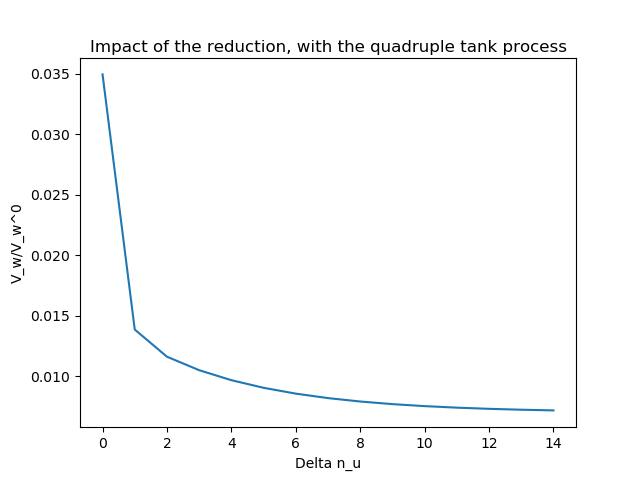
\includegraphics[width=0.9\linewidth]{lin_sys_reduction_seq_control_len}
  \caption{Impact of the variable $\Ninputs$ over the size of the possible state of the reduced system. It does not worth to take $\Ninputs$ greater than 1 since the boundaries of the reduce system does not decrease that much and the complexity of the model exponentially dependant of the number of controls.}
  \label{reduced_system_bounds}
\end{figure}

The next table summaries the gains and loses of this reduction on the previously established criteria.

\begin{tabular}{ l|ll }
& Initial model & Reduced model\\ \hline
Nodes & $\prod_{i=1}^n N_i$ & $\left | U \right |^{\Ninputs} \prod_{i=1}^{n_c} N_i $\\ 
$|U|$ & $n_u$ & $n_u$\\
$V_w$ &  & bigger \\
\end{tabular}

\section{Notes for the future}
Abstractions of asymptotically stable system present a disadvantage on the multiagent control side, for some controls, if the state does not evolve any more, the abstraction will take self loops.
In term multi agent control this make the problem more complex as the control generation: self loops tend to create systems that are asynchronous with all the problems that might occurs because of this (basically one of the agent might be be stopped).

Self loops are not desirable.

Self loops hide any time information (that is why I have been working on the time information chapter).

In the case of the reduction of the abstraction.
\section{Discussion}

\subsection{Reduction}
As it as been mentioned in the introduction, the "abstraction reduction" does not always create smaller abstractions.
This depends on the type of inputs (discrete, continuous), the number of dimension of inputs, the dimension of the suppressed subspace of the state space and the initial discretization of it.

\subsection{Covering/Overlap in the state space}
When we replace the knowledge of part of the state by the estimation of the state based on inputs, there can be no equivalent discretization of the state space.
Mainly because 2 input sequences can produce reached sets that overlaps.
These overlap (see \ref{fig:overlapp}) cannot happened in discretization of the state space without any memory (the state is supposed to belong to one and only one observation).

We will see later that it can bring to improvement of the size of the abstraction in practice.

\begin{figure}
\centering
\begin{minipage}[b]{0.49\textwidth}
	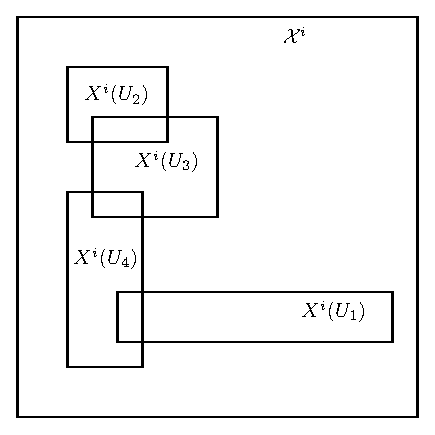
\includegraphics[width=\textwidth]{chapters/abstraction_reduction/overlapp_disc.eps}
\end{minipage}	
\begin{minipage}[b]{0.49\textwidth}
	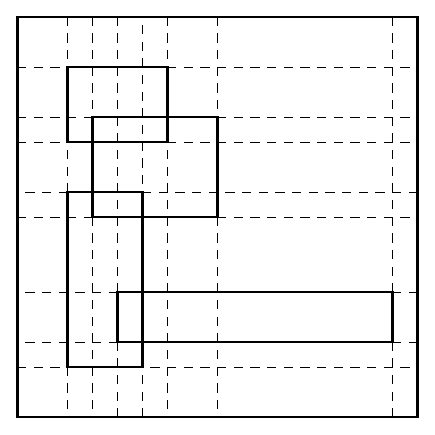
\includegraphics[width=\textwidth]{chapters/abstraction_reduction/overlapp_disc2.eps}
\end{minipage}	
\caption{For the abstraction on the right, the reached sets overlapps. The equivalent discretization of the state space on the left create an abstraction of 72 symbols for 4 symbols in the case of the reduction.}
\end{figure}

Dynamic of the successor volume.

Self loops -not cool for multi agent task, lose the time information.
Abstractions of asymptotically stable system present a disadvantage on the multiagent control side, for some controls, if the state does not evolve any more, the abstraction will take self loops.
In term multi agent control this make the problem more complex as the control generation: self loops tend to create systems that are asynchronous with all the problems that might occurs because of this (basically one of the agent might be be stopped).

size of invariants in the 

%TODO GRAPH TO SHOW IT (I can also do it for the second integrator)

We will see that in some case it produce way smaller abstraction.

\subsection{Error sensitivity}
As we do not observe $\xunobs$, the reduced abstraction is not sensible to the measurement error on $\xunobs$. More over, as $\xunobs$ does not have a direct impact on the measurement, the error on $\xunobs$ impact the observation as a cumulative error.

During the reduction of the abstraction process, the admissible noise magnitude remain the same. However, the constraints are different as the error does not have any more a direct impact on the state but can be propagating.
In this part, we will try to establish what are the new constraints that does apply on the noise.

If there is no closed form solution to it, do it for a stupid system or for the quad.

\subsection{Reachability/Controllability}
Reachable sets are computed with the invariant set. As the invariant set is an over approximation of the state, it is always possible to find a discretization of the unobserved subspace that create less successors than the estimation of the state.
This might results in an abstraction that is unusable whatever the number of memories we are using or the sampling rate of the model.

\subsection{Notes}
Self loops are not desirable.

Self loops hide any time information (that is why I have been working on the time information chapter).

In the case of the reduction of the abstraction.
\newcommand{\xo}{\vect{x}^o}%
\newcommand{\xr}{\vect{x}^r}%
%
\newcommand{\Ao}{A_o}%
\newcommand{\Ar}{A_r}%
\newcommand{\Aro}{A_{ro}}%
%
\newcommand{\Bo}{B_o}%
\newcommand{\Br}{B_r}%
%
\newcommand{\Eo}{E_o}%
\newcommand{\Er}{E_r}%
\newcommand{\Ero}{E_{ro}}%
%
\newcommand{\Xr}{X_r}%
%
\newcommand{\Xrinv}{\mathcal{X}_r}%
\newcommand{\xrinf}{\minf{\x}_r}%
\newcommand{\xrsup}{\msup{\x}_r}%
%
%
\newcommand{\Wsup}{\msup{W}}%
\newcommand{\Winf}{\minf{W}}%
\newcommand{\Wk}{W_k}%
%
\renewcommand{\wr}{\vect{w}^r}%
\newcommand{\wrsup}{\msup{\vect{w}}^r}%
\newcommand{\wrinf}{\minf{\vect{w}}^r}%
\newcommand{\Wrsup}{\msup{W}^r}%
\newcommand{\Wrinf}{\minf{W}^r}%
\newcommand{\Wrk}{W^r_k}%
%
\newcommand{\z}{\vect{z}}%
\newcommand{\zk}{\z_k}%
\newcommand{\zkn}{\z_{k+1}}%
%
\newcommand{\xkn}{\x_{k+1}}%
\newcommand{\xk}{\x_{k}}%
\newcommand{\uk}{\u_{k}}%
\newcommand{\wk}{\w_{k}}%
\newcommand{\yk}{\y_{k}}%
\newcommand{\ykn}{\y_{k+1}}%
%
\newcommand{\Z}{\mathbf{z}}%
\newcommand{\Zk}{\Z_k}%
\newcommand{\Zkn}{\Z_{k+1}}%
\newcommand{\hk}{\vect{h}_{k}}%
\newcommand{\h}{\vect{h}}%
\newcommand{\wnoise}{\msup{\sigma}}%
%
\newcommand{\size}{N}%
\newcommand{\norminf}[1]{\left\|#1\right\|_{\infty}}%
%
\newcommand{\xui}{\minf{\x}^U_r}%
\newcommand{\xus}{\msup{\x}^U_r}%
\newcommand{\An}{\mathcal{A}^r_n}%
\newcommand{\Bn}{\mathcal{B}^r_n}%
\newcommand{\En}{\mathcal{E}^r_n}%
\newcommand{\xuki}{\minf{\x}^{U_k}_r}%
\newcommand{\xuks}{\msup{\x}^{U_k}_r}%
\newcommand{\xuk}{\x^{U_k}_r}%
%
\newcommand{\ANoise}{\Omega}%
\newcommand{\NoiseSet}{\mathcal{W}}%
\newcommand{\infseq}{\omega}%
%
\newcommand{\sykn}{\msup{\y}_{k+1}}%
\newcommand{\iykn}{\minf{\y}_{k+1}}%
%
\newcommand{\filter}{\mathcal{F}}%
%
\section{Error sensitivity}
%
In the previous sections, we have been using a dynamical model to build an abstraction $S_a$. In this part, we will solve the opposite problem:  we would like to find all the admissible models that can be alternatively simulated by $S_a$.
In our case, we will find all the admissible models with the same dynamic as the initial model $S$ but with a different noise set.

As we do not observe $\xunobs$, the error on $\SSunobs$ does not have a direct effect on the input extended state abstraction.
However, it does have an impact as the dynamics on $\SSunobs$ influence the one on $\SSobs$.
In this part, we will see that the admissible noise set is actually bigger (in the sense of inclusion) than the noise set used for the modellisation.

We will consider the system definition \ref{lin_sys_decoupled} with noise sets and input sets 2 monotone sets expressed by:
\begin{equation}
\begin{aligned}
\U &= [\minf{\u},\msup{\u}]\\
\W &= [\minf{\w},\msup{\w}]\\
\end{aligned}
\end{equation}

%% Explain what is the definition of an admissible noise
A sequence of noise is admissible if it does not violate the transitions of the abstraction for any possible trajectory.
In our case, this mean that for any sequence of noise, the observation of the next state must belong to the monotone interval of observations.
This can be expressed in this way:
\begin{equation} \label{valid_transition}
\ykn \in [\iykn,\sykn]
\end{equation}
where 
\begin{align*}
\sykn &= C \msup{\x}_{k+1} = 
C A 
\begin{bmatrix}
\xo_{k} \\
\xrsup
\end{bmatrix}
+ C B \uk + C E \msup{\w}
\\
\iykn &= C \minf{\x}_{k+1} 
= C A 
\begin{bmatrix}
\xo_{k} \\
\xrinf
\end{bmatrix}
+ C B \uk + C E \minf{\w}
\\
\ykn &= C \x_{k+1}
= C A 
\begin{bmatrix}
\xo_{k} \\
\xr
\end{bmatrix}
+ C B \uk + C E \wk
\end{align*}

We will now use the inequalities \ref{valid_transition} to get conditions over the noise:
\begin{align}
\ykn \mleq \sykn
& \Leftrightarrow
0 \mleq \sykn - \ykn
\nonumber \\
& \Leftrightarrow
0 \mleq
C A \begin{bmatrix} 0 \\ \xrsup-\xr_k \end{bmatrix}
+ C E (\msup{\w} -\wk)
\nonumber \\
& \Leftrightarrow
0 \mleq
\Aro ( \xrsup-\xr_k ) + C E (\msup{\w} -\wk)
\label{equi_upp}
\end{align}
We would like to have a condition over the noise only. However, the process $\xr_k$ depend on the input $\uk$. Therefore, we will introduce the variable $\zk$ defined by:
\begin{equation}
\zkn = \Ar \zk + \Er \wk + \Br \msup{\u}
\end{equation}
Thanks to the monotone property and to $\uk \mleq \msup{\u}$, for any trajectory if $\x_0 \mleq \z_0$, then:
\begin{equation}\label{process_ineq}
\xk \mleq \zk
\end{equation}
Lets define $\zk^* = \zk + (\Ar-I)^{-1} \Br \msup{\u}$, for all $k\in \mathbb{N}$:
\begin{equation}
\zkn^* = \Ar \zk^* + \Er \wk
\end{equation}

Then by using the inequality \ref{process_ineq} and equivalence \ref{equi_upp}, we have the following implication:
\begin{equation}
\Aro (\zk^* - (\Ar-I)^{-1} \Br \msup{\u} ) + CE \wk 
\mleq \Aro \xrsup + CE \msup{\w}
\Rightarrow 
\ykn \mleq \sykn
\end{equation}

\newcommand{\sig}{\sigma}
\newcommand{\ssup}{\msup{\sig}}
\newcommand{\sinf}{\minf{\sig}}
Finally, we have that:
\begin{equation}
\Aro \zk^* + CE \wk 
\mleq 
\ssup
\Rightarrow 
\ykn \mleq \sykn
\label{impl_upp}
\end{equation}
with $\ssup = \Aro ( \xrsup + (\Ar-I)^{-1} \Br \msup{\u} ) + CE \msup{\w}$

The same implication can be done with the lower bound of $\yk$:
\begin{equation}
\Aro \zk^* + CE \wk 
\mleq 
\sinf
\Rightarrow 
\ykn \mleq \sykn
\label{impl_low}
\end{equation}
with $\sinf = \Aro ( \xrinf + (\Ar-I)^{-1} \Br \minf{\u} ) + CE \minf{\w}$

We will express these 2 implications with a filter inequality.
Let the following filter $\filter$:
\begin{equation}
\filter:
\left\{
\begin{split}
\zkn^* &= \Ar \zk^* + \Er \wk \\
\hk &= \Aro \zk + CE \wk \\
\end{split}
\right.
\end{equation}
Then implications \ref{impl_upp} and \ref{impl_low} are satisfied if the output of the filter $\filter$ is in $[\sinf,\ssup]$ for all the timesteps.
The set $\W_a$ of noise sequences that verify:
\begin{equation}
\forall k \in \mathbb{N}, \h_k \in [\sinf,\ssup]
\end{equation}
is a subset of the admissible noise sequences.


By linearity of the filter, we know that if the sequences $\{\wk^1\}_{k\in \mathbb{N}}$ and  $\{\wk^2\}_{k\in \mathbb{N}}$ are admissible, then the sequence defined by $\{a\wk^1 + b\wk^1\}_{k\in \mathbb{N}}$ with $a,b>0$ and $a+b = 1$ is an admissible noise sequence.
Lets now consider the bode $G$ function of the filter $\filter$ and the set $\W'$ defined by:
$$\W_G = 
\{ 
\{G(w) cos(w k + \phi)\}_{k \in \mathbb{N}} 
\mid \phi \in [0,2\pi], w \in [0,2\pi] \}
$$
We have that the convex polyhedra defined by the set $\W_G$ is a subset of the admissible noise set.
This result give us a practical criteria over the set of admissible noise sequences.
It will also help us to understand some experiments.

Please note that the maximum constant noise remains unchanged.
However, noises of higher frequencies can have greater magnitudes than the one modelled initially. 


\comment{Add property that the convex polyhedra of the sinusoidal signals with magnitude less than $u$ correspond to the set of all signals so that $u_n<u$ for all $n$.}
%
%
\chapter{Backward reachability algorithm}
\section*{Notation}
\begin{tabular}{ll}
FTS:& Finite Transition System\\
LTL:& Linear Temporal Logic\\
DBA:& Deterministic B\"uchi Automaton\\
NBA:& Nondeterministic B\"uchi Automaton\\
BFS:& Breadth First Search\\
DFS:& Depth First Search\\
\end{tabular}

For $X,Y$ two sets, $X|_Y = \{x \in X \mid x \notin  Y \}$, $2^X$ is the power set of $X$.

Let a graph $G = (V,E)$.
For a node $x \in V$, $Post(x)$ and $Pre(x)$ correspond respectively to the set of successors and predecessors of $x$. 
For a set of nodes, we define $X \subseteq V$, $Post(X) = \bigcup_{x \in X} Post(x)$, $\outpost(X) = Post(X) \setminus X$, $Pre(X) = \bigcup_{x \in X} Pre(x)$ and $\inpre(X) = Pre(X) \setminus X$.

For $X_1,\dots,X_n$ n sets and $Y \subset X_1 \times \dots \times X_n$, lets define the projection of $Y$ on $X_i$ with $Y|_{X_i} = \{x_i \mid (x_1,\dots,x_n) \in Y\}$.

\section{Introduction}

This part is presenting the planning under strong fairness constraints.

\cite{de2010generalized}
\cite{patrizi2013fair}


By modelling the system in this way we are losing a lot of expressiveness power of the LTL. However, the complexity remain more or less the same than before 2EXPTIME-complete ($\mathcal{O}(2^{2^{n^k}})$) (\textit{not so sure about it, double check information}).

\section{Linear Temporal Logic}
Linear Temporal Logic (LTL) is specification language first introduced in \cite{pnueli1977temporal}. Since then it has been widely used in robotic motion and action planning thanks to its expressiveness.

LTL property are defined inductively:

$$ \varphi ::= 
\true \mid 
a \mid 
\varphi_1 \land \varphi_1 \mid
\lnot \varphi \mid
\LTLnext \varphi \mid
\varphi_1 \LTLuntil \varphi_2$$

\textit{define each symbol inside it.}

\begin{nameddef}{LTL property}
The truth of an LTL property $\varphi$ is defined by:
\begin{tabular}[b]{rcl}
$(\sigma,k) \vDash a$ & $\leftrightarrow$ & $a \in S_k$\\
$(\sigma,k) \vDash \lnot \varphi$ & $\leftrightarrow$ &  $(\sigma,k) \nvDash  \varphi$ \\
$(\sigma,k) \vDash \LTLnext \varphi$ & $\leftrightarrow$ &  $(\sigma,k+1) \vDash  \varphi$ \\
$(\sigma,k) \vDash \varphi_1 \lor \varphi_2$ & $\leftrightarrow$ &  $(\sigma,k) \vDash  \varphi_1$ or $(\sigma,k) \vDash  \varphi_2$ \\
$(\sigma,k) \vDash \varphi_1 \LTLuntil \varphi_2$ & $\leftrightarrow$ &  $\exists k' \in \left [k, +\infty \right ] , (\sigma,k') \vDash \varphi_2$ and \\
& & $\forall k'' \in (k,k'), (\sigma,k'') \vDash \varphi_1$ \\
\end{tabular}
\end{nameddef}

We also define some useful operators: \textit{eventually} $\LTLeventually \varphi = \true \LTLuntil \varphi$, \textit{always} $\LTLalways \varphi = \lnot \LTLeventually \lnot \varphi$, \textit{implication} $\varphi_1 \LTLimply \varphi_2 = \lnot \varphi_1 \lor \varphi_2$.
More details can be found in chapter 5 of \cite{principlemodelchecking}.

All the power of such a language lie in the ability to transform a human writeable formula in a machine manipulable data. LTL formula can be translated to an automaton structure that can be easily manipulated with discrete models. The problem of path planning is then reduced to finding a path in graph.

\subsection{Translation to \buchi{} automaton}

Give theorem that show that every LTL formula can be translated in a \buchi{} automaton.

Talk about what kind of LTL fragment can be translated in a deterministic \buchi{} automaton.
Cite the complexity of such algorithms.

Talk about other structure that might have been more relevant for your work (more deterministic), ex: Rabin automaton.

\section{Reachability algorithm}

\subsection{Previous works}

Modelled as a global reactive game. Generalized Reactive.
However these methods are adapted for action non determinism, movement non determinism can be more complex.

Talk about why they have been doing this? Deal with uncertainty about the environment.

Why did you chose LTL?
Why did you chose B\"uchi Automaton?
Talk about other solutions that might have been smarter.

\subsection{Product automaton for nondeterministic system}

The product automaton for an nondeterministic FTS is defined as follow:

\begin{nameddef}{Finite Transition System}
$\mathcal{T}_c = (X,X_0,U, \transition, Y,H)$
where:
\begin{itemize}[noitemsep,nolistsep]
\item $X$ is a set of states;
\item $X_0 \subset X$ a set of initial states;
\item $U$ a set of inputs;
\item $\transition \subseteq X \times U \times X$ a transition relation ;
\item $Y$ a set of outputs;
\item $H:X \rightarrow Y$ an output map.\popQED
\end{itemize}
\end{nameddef}

Let $H^{-1}$ defined by $H^{-1}(\mathcal{O}) = {x \in X \mid H(x)=\mathcal{O}}$ for $\mathcal{O} \in Y$.

\begin{nameddef}{Nondeterministic B\"{u}chi Automaton}
$\mathcal{A}_{\varphi} = (Q, Q_0, 2^{AP}, \delta, \mathcal{F})$
where:
\begin{itemize}[noitemsep,nolistsep,topsep=0pt,after=\relax]
\item $Q$ finite set of states;
\item $Q_0 \subset Q$ a set of initial states;
\item $2^{AP}$ the alphabet;
\item $\delta: Q \times 2^{AP} \times Q$ a transition relation ;
\item $\mathcal{F}$ set of accepting states.\popQED
\end{itemize}
\end{nameddef}

Nota: if $\forall q \in Q, \forall a \in 2^{AP}, | \delta(a,q) | \leq 1$, then $\mathcal{A}_{\varphi} = (Q, Q_0, 2^{AP}, \delta, \mathcal{F})$ is a \textit{Deterministic B\"uchi Automaton} (DBA).

\begin{nameddef}{Product of a NBA and a FTS}
The product automaton $\mathcal{A}_p$ of the NBA $\mathcal{A}_\varphi$ and the non deterministic FTS $\mathcal{F}_c$ is defined by
$\mathcal{A}_p = \mathcal{T}_c \otimes \mathcal{A}_\varphi
= (Q',Q_0',\delta',\mathcal{F}')$
where
$Q' = X \times Q$ is the set of states,
$Q_0' = X_0 \times Q_0$ is the set of initial states,
$\mathcal{F}' = X \times \mathcal{F}$ the acceptance set,
$\delta' \subseteq Q' \times U \times Q'$
is the transition relation defined by
$\left \langle x',q' \right \rangle \in \delta'(\left \langle x,q \right \rangle ,u)$
iff $x' \in Post_u(x)$, $q' \in \delta(q,L_c(x'))$ and 
$$\forall h \in H(Post_u(x)),\exists y \in H^{-1}(h) \cap Post_u(x), \delta(q,L_c(y)) \neq \emptyset$$
\end{nameddef}

Roughly speaking, a $u$-transition in the product automaton is valid iff for every observation of the successors of a $u$-transition of the FTS, there exists a valid transition in the B\"uchi Automaton.

\begin{nameddef}{Product of 2 FTS}
The product automaton $\mathcal{F}_p$ of 2 non deterministic FTS $\mathcal{F}_1$ and $\mathcal{F}_2$ is defined by
$\mathcal{F}_p = \mathcal{F}_1 \otimes \mathcal{F}_2
= (X',X_0',U',\delta',Y',H')$
where
$X' = X_1 \times X_2$ is the set of states,
$X_0' = X_{10} \times X_{20}$ is the set of initial states,
$U' = U_1 \times U_2$ the input set,
$Y' = Y_1 \times Y_2$ the output set,
$H': X_1,X_2 \rightarrow (H_1(X_1),H_2(X_2))$ the output map,
$\delta' \subseteq X' \times U \times X'$
is the transition relation defined by
$\left \langle x_1,x_2 \right \rangle \in \delta'(\left \langle x_1',x_2' \right \rangle,\langle u_1,u_2 \rangle)$ iff $x_1 \labelledtransition{u_1} x_1'$ and $x_2 \labelledtransition{u_2} x_2'$.
\end{nameddef}


\subsection{LTL Planning under Strong Cyclic \\Fairness Constraints}

\cite{de2010generalized}
\cite{patrizi2013fair}

Fully Observable Non-Deterministic Planning:  FOND

The guaranties that an nondeterministic planner must fulfil are:
\begin{itemize}[noitemsep,nolistsep]
\item \textbf{Completness.}
\item \textbf{Soundness.} Every given solutions are correct
\item \textbf{Correctness.} 
\item \textbf{Fairness.}
\end{itemize}

For which LTL formula we will be able to find a solution if the solution exists?

Unlike most of algorithms, the strong fairness property over inner loops of the product automaton are not fair for every combinations of controls.
Finding a closed and proper solution for that plan is not a sufficient condition in our case. 
We need to insure that every cycles in the final system (system composed of the plan and of the product automaton) does not deadlock the system.

\subsection{Related work}
How to deal with nondeterminism?
Different approaches:
\begin{itemize}
\item general game formulation: GR(1) (however, the formulation does not fit to our needs): in \cite{de2010generalized} and \cite{Kissmann2009}, the strong fairness property is expressed thanks in a LTL formulation, however it presuppose a knowledge about cyclic actions fairness property, this is adapted to action planning where we know that if the action is infinitely repeated, then the action will success infinitely often. This does not really fit any motion planning non determinism where the fairness property depend on a control configuration over the cells. Using this kind of framework will force us to go through all the possible action combinations and determine which one is fair.
\item Fixed point ($\mu$-calculus that is related to the GR formulation as well).
\item \cite{fu2011simple} is solving the FOND problem in the case of strong fairness assumption. This assumption is global, this is not the case for us as some of some control configurations might be unfair. The fairness property is local in our case.
\end{itemize}

What I did is an adaptation of the \cite{fu2011simple} with a backward reachability algorithm.

\subsection{Premilinaries}

\subsubsection{Graph theory}
Fully observed non deterministic: thats means that the B\"uchi automaton should be deterministic.

\begin{nameddef}{Strong connectivity}
The directed graph $G = (V,E)$ is strongly connected iff for every nodes $u,v \in V$ there exists a path from $u$ to $v$.
\end{nameddef}


%% FAIRNESS PROPERTY
\begin{nameddef}{Fairness property}

\end{nameddef}

\subsection{Fix point algorithm}
%% introduce the fixed point property, make a link between mu calculus
%% I just need a property that establish the working conditions for the fixed point property and the finitness of the algorithm.

% definition of a fixed point
% definition of the least fixed point
% definition of a monotonic fonction t: 2^S -> 2^S
% theorem tarski-knaster for the fixed point of a monotonic function -> existence of the least fixed point
% include the finitness directely inside the theorem, or as a note
In the next parts we will use operations over sets of nodes in the graph. In order to find subset of nodes where property are verified, we will use fixed point computation.

We say that $b$ is a \inlinedef{fixed point} of the functional $\tau$ if $\tau(b) = b$.
For a set $S$, the functional $\tau: 2^S \rightarrow 2^S$ is  \inlinedef{monotonic} iff $\forall a,b \in 2^S, a \subseteq b, \tau(a) \subseteq \tau(b)$.
In \cite{tarski}, it is shown that for a monotonic functional $\tau$,
the set of fixed points has a least and greatest element denoted by $\mu \tau$ and $\nu \tau$ respectively:

\begin{namedtheo}{Tarski-Knaster}\label{th:tarski}
Let $\tau:2^S \rightarrow 2^S$ a monotonic functional:
\begin{itemize}
\item $\mu \tau = \bigcap \{b \subseteq S \mid \tau(b) \subseteq b\} = \bigcup_{\alpha \in On} \tau^{\alpha}(\emptyset)$
\item $\nu \tau = \bigcup \{b \subseteq S \mid b \subseteq \tau(b) \} = \bigcap_{\alpha \in On} \tau^{\alpha}(S)$
\end{itemize}
where $\tau^{\alpha}$ is the $\alpha^{th}$ composition of $\tau$ and $On$ the class of ordinals.
\end{namedtheo}
In our case, $S$ is the finite set and $On = \leftint 1,|S|\rightint$. 
In this case, the theorem ensure the existence and the finiteness of the least fixed point computation.
Please note that if $a$ and $b$ are least fixed points of the monotonic functional $\tau$, then $a \subseteq b$ and $b \subseteq a$, which means that $a=b$, which means that the least fixed point is unique.

\subsection{All non deterministic plans can be decomposed in strongly connected cycles}

\newcommand{\planningdomain}{\ensuremath{ \tuple{\langle S, S_0, \mathcal{A}, \gamma \rangle} }}

\newcommand{\controller}{\ensuremath{\tuple{ \langle C, c_0, \Gamma, \Lambda, \delta, \Omega \rangle}}}

\newcommand{\planningproblem}{\ensuremath{\tuple{ \langle \mathcal{D}, G \rangle}}}
I need to define a plan, the model.

\begin{nameddef}{Nondeterministic Planning Domain}
A nondeterministic planning domains is a tuple 
$\mathcal{D} = \planningdomain$
with
$S$ the set of states,
$S_0$ the set of initial states,
$\mathcal{A}$ the set of actions and
$\gamma : S \times \mathcal{A} \rightarrow 2^S$ the transition function.
\end{nameddef}

Note that as the model is nondeterministic, for $(s,a) \in S \times \mathcal{A}$ we might have $|\gamma(s,a)|>1$.

\begin{nameddef}{Finite-State Controller (FSC)}
For a nondeterministic planning domain
$\mathcal{D} = \planningdomain$,
$\Pi = \controller$ is a finite-state controller where
$C$ is the set of states,
$c_0$ is the initial state,
$\Gamma = S$ is the controller input alphabet,
$\Lambda = Act$ is the output alphabet,
$\delta: C \times \Gamma \rightarrow C$ is the transition function and 
$\Omega: C \rightarrow \Lambda$ is the output function.
\end{nameddef}

\begin{nameddef}{Non terminating nondeterministic Problem}
A nonterminating nondeterministic problem $P = \planningproblem$ where $\mathcal{D}$ is a nondeterministic planning problem and $G \subseteq S$ is the goal subset. A finite-state controller $\Pi$ is a solution of $P$ if every $\Pi$-runs goes infinitely to the subset $G$ ($\forall \pi \in \Pi-runs, Inf(\pi) \cap G \neq \emptyset$).
\end{nameddef}

\begin{nameddef}{Terminating nondeterministic Problem}
A nondeterministic problem $P = \planningproblem$ where $\mathcal{D}$ is a nondeterministic planning problem and $G \subseteq S$ is the goal subset. A finite-state controller $\Pi$ is a solution of $P$ if every $\Pi$-runs goes to $G$ in a finite time.
\end{nameddef}

FTC $\Pi$ is said to be \textit{closed} if every reachable state is associated with a control  action, $\Pi$ is \textit{proper} if the the goal set is reachable from every state and $\Pi$ is said \textit{fair} if the goal is reachable in finite time from every nodes.
We will say that the FSC $\Pi$ is a valid solution of the nondeterministic problem $\mathcal{D}$ if $\Pi$ is \textit{closed}, \textit{proper} and \textit{fair}.

It is shown in \cite{patrizi2013fair} that every non-terminating nondeterministic planning problem $P$ can be solved like a nondeterministic planning problem $P'$ where the the initial set of $P'$ correspond to the union of the initial set and the goal set.

In this next sections we will proof that every plans can be decomposed in strong cyclic components.
Then we will investigate the necessity of the fairness property.
Finally, we will use all these properties in order to justify the planning algorithm that we used.

\subsubsection{Strong cycle decomposition}
\textit{Try to specify a bit more the language of the graph decomposition.
Modules/components/subcomponents.}

In this section we will use a constructive argument to show that every plan can be decomposed in strong cyclic components.

Let a $\mathcal{D} = \planningdomain$ a nondeterministic planning domain, $\Pi = \controller$ a finite-state controller that is a valid solution of the terminating nondeterministic planning problem $P = \planningproblem$.

The main idea of the decomposition is to find every strong cyclic components of $\mathcal{D}$ that deterministically bring us to the goal set of nodes.
To do this we will recursively find all the smallest strongly connected cycles that deterministically bring the state closer to the goal set.
The description of the construction will be followed by a proof that for a valid plan  all the nodes of the plan belong to the decomposition.

\paragraph{Strongly connected components,} they will be found using fixed point algorithm.
Let $F_{t \rightarrow g}$ defined for $g,t \subseteq S$ by:
\begin{equation}
\begin{array}{llll}
F_{t \rightarrow g} :& 2^S & \rightarrow & 2^S\\
 & x &  & (Post(x) \cap S \setminus_g) \cup t
\end{array}
\end{equation}


For $x \subseteq y$ we have $F_{t \rightarrow g} (x) \subseteq F_{t \rightarrow g}(y)$, so $F_{t \rightarrow g}$ is a monotonic functional and theorem \ref{th:tarski} ensure that $F_{t \rightarrow g}$ have a unique least fixed point.
As the cardinality of $S$ is finite, we can compute the fixed point of $F_{t \rightarrow g}$ in a finite time
(\textit{Can I talk about computability instead of computable in finite time?}).

\textit{Do I really need to prove the strong connectivity ?}
\begin{prop}
For $t,g \subseteq S$, if $t$ is a strongly component of a graph $G$, the least fixed point of $F_{t \rightarrow g}$ is strongly connected.
\end{prop}

\begin{proof} 
Let $x \subseteq S$ the least fixed point of $F_{t \rightarrow g}$.
By definition of $F_{t \rightarrow g}$, there exist a path from all the nodes in $t$ to all the nodes.
We need now to show that there always exists a path from every nodes in $x$ to $t$ or $g$.
As the 
\end{proof}

Let $\mathcal{F}_g(t) = F_{t \rightarrow g}$ the least fixed point of $F_{t \rightarrow g}$.
$\mathcal{F}_g(t)$ correspond to the smallest strongly connected cycle containing the subset $t$ that can reach the subset $g$.

Lets now define the decomposition of the plan in strongly connected components.

For $g \subseteq S$, let $\mathfrak{F}_g = \{ \mathcal{F}_g(\{n\}) \mid n \in \inpre(g) \}$.
$\mathfrak{F}_g$ correspond to the set of all the smallest strongly connected components that deterministically go to the subset $g$.
\textit{Do I really need the uniqueness property.}
The uniqueness of  $F_{t \rightarrow g}$ least fixed point ensure the uniqueness of $\mathfrak{F}_g$.

For a set of set $X \subset 2^{2^S}$, let $\tilde{X} = \bigcup_{x \in X} x$.

Let the sequence $\{\mathcal{K}_i\}_{i \in \mathbb{N}}$ define by:
\begin{equation*}
\mathcal{K}_{i+1}  = \mathfrak{F}_{\tilde{\mathcal{K}}_i} \cup \mathcal{K}_i
\textrm{, }
\mathcal{K}_0 = G
\end{equation*}
for $i \in \mathbb{N}$. 

By observing that,
\begin{equation}
\begin{array}{llll}
H : &2^{2^S} &\rightarrow &2^{2^S}\\
&X & & \mathfrak{F}_{\tilde{X}} \cup X \cup \{ g \}
\end{array}
\end{equation}
is a monotonic functional on a finite set $2^{2^S}$ and by using theorem \ref{th:tarski}, we know that the least fixed point of $H$ exist and is computable in finite time.
As $\mathcal{K}_i = H^i(\emptyset)$, we can deduce that the sequence $\{\mathcal{K}_i\}_{i \in \mathbb{N}}$ is converging to an element $\mathcal{K}^\star \in 2^{2^S}$ in a finite number of steps.

$\mathcal{K}^\star$ corresponds to the decomposition of the plan in strongly connected cycles.
\textit{I don't know if each of the fixed point are strong cycles, also I don't use this property.}

We need now to be sure that the decomposition of the plan is complete \textit{Are you sure of this word?}, ie all the nodes of the plan belong to the decomposition:
\begin{prop}
For a valid plan, $\tilde{\mathcal{K}}^\star = S$.
\end{prop}
\begin{proof}

By definition of $\mathcal{F}_g$, we have:
\begin{equation}
n \in S \setminus g \Leftrightarrow \mathcal{F}_g(\{n\}) \neq \emptyset
\end{equation}
This imply that:
\begin{equation} \label{eqn:equiv_f_empty}
\mathfrak{F}_g = \emptyset \Leftrightarrow Pre(g) = \emptyset
\end{equation}

Moreover, by definition of $\mathfrak{F}_g$:
\begin{equation} \label{eqn:f_empty}
\tilde{\mathfrak{F}}_g \cap g = \emptyset
\end{equation}
For $\mathcal{K}^\star$, as $\mathcal{K}^\star = \mathfrak{F}_{\tilde{\mathcal{K}}^\star} \cup \mathcal{K}^\star$ and thanks to equality \ref{eqn:f_empty}, we have $\mathfrak{F}_{\tilde{\mathcal{K}}^\star} = \emptyset$.  
By using equivalence \ref{eqn:equiv_f_empty}, we prove that $Pre(\tilde{\mathcal{K}}^\star) = \emptyset$.

By using the definition of $\mathcal{F}_g$,
we can show that for all $F \in \mathcal{K}^\star \setminus \{G\}$, $\outpost(F) \subset \tilde{\mathcal{K}}^\star$.
This imply that $\outpost(\tilde{\mathcal{K}}^\star) = \outpost(G)$.
As the problem is a terminating problem, $\outpost(G) = \emptyset$, this imply that 
$\outpost(\tilde{\mathcal{K}}^\star)  = \emptyset$.

As $\inpre(\tilde{\mathcal{K}}^\star)  = \emptyset$ and $\outpost(\tilde{\mathcal{K}}^\star)  = \emptyset$, all the nodes outside $\tilde{\mathcal{K}}^\star$ are not connected to $G$.
Then the validity of the plan prove that all the nodes outside   $\tilde{\mathcal{K}}^\star$ cannot belong to the plan.
\end{proof}


\begin{figure}
	\center
	\includestandalone[width=0.7\textwidth]{plan_decomposition}
	\caption{Decomposition of the plan in strong cycles components (red boxes) and transitions between them (blue arrows). The agent goes from area \textit{init} to stay in the set \textit{G} (in the green box) following the controls actions (in black arrows).}
	\label{fig:environment}
\end{figure}

\subsubsection{Fairness property}
In the previous section we have settled the decomposition of the graph in strong cyclic components.
We will now investigate when these strong cyclic components need to verify fairness property.

If the plan $P$ is a solution of the nondeterministic planning problem, then every run reach the set $G$ in a finite time.
Lets $\mathcal{K}^\star$ be the previously defined decomposition of the plan $P$.
In the following paragraph, we will establish when the fairness property must be verified for each element of $\mathcal{K}^\star$.

Let define the following subsets of $\mathcal{K}^\star$:
\begin{align}
\mathcal{K}_{unfair} &= \{ F \in \mathcal{K} \mid F \subseteq G \}\\
\mathcal{K}_{fair} &= \mathcal{K}^\star \setminus \mathcal{K}_{unfair}
\end{align}

\begin{prop}
All the elements of $\mathcal{K}^\star \setminus {G}$ verify fairness property.
\end{prop}

\begin{proof}
Let $\Pi$ a finite-state controller that is a solution of the problem $P$ and $\mathcal{F} \in \mathcal{K}^\star \setminus \{G\}$ a $\Pi$-reachable set of nodes.
If $\mathcal{F}$ does not verify the fairness property we can choose a $\Pi$-run $\pi = \{s_i\}_{i\in\mathbb{N}}$ so that it exists $k\in\mathbb{N}$ where $\forall k'>k, s_{k'} \in \mathcal{F}$, this means that $Inf(\pi) \subset \mathcal{F}$

As $G \cap \mathcal{F} = \emptyset$, we have $Inf(\pi) \cap G =\emptyset$, so this run is not accepted, which contradict the fact that $\Pi$ is a solution of $P$.
\end{proof}


\subsubsection{Fairness property of product systems}
In our case the systems that that we will use are products of FTS and BA. We will have the information about the fairness property for each of the system, so we need to investigate the link between the fairness property of the product system and all the systems.

\begin{prop}
Let $S = S_1 \otimes \dots \otimes S_n$ the product automaton of $n$ finite transition systems (FTS or BA) $(S_1,\dots,S_n)$.
Let $\mathcal{F}$ a strong cyclic component of $S$ obtained with the strong cyclic decomposition.
If $\mathcal{F}$ is unfair then $\mathcal{F}|_{S_i}$ is unfair for $i = 1,\dots,n$.
\end{prop}

\begin{proof}
If the subsystem $S_j$ is fair for $j \in \llbracket 1,n \rrbracket$ on $\mathcal{F}|_{S_j}$, then all the paths exit $\mathcal{F}|_{S_j}$ in a finite time, this imply that all the runs on the product automaton $S$ exits $\mathcal{F}$ in finite time as well.
\end{proof}

Ones should note that this property is valid for products of systems such as finite transition system or \buchi{} automaton (or any combination of them).

For a \buchi{} automaton, all the cycles are unfair.
For a FTS, we will specify the fairness property with a function that return the maximal time that the system can spend in a subset of nodes
(for an unfair strong cycle of the FTS, this time will be equal to $+\infty$).

We can formally define the escape function for the product automaton:
\begin{property}
The escape function of the product automaton $S$ is:
$$T_{escape}^S = \min{T_{escape}^{S_i}}$$
where $T_{escape}^{S_i}$ is the escape function of the system $S_i$.
\end{property}

\begin{proof}
\textit{I need to provide something more rigorous.}
If the faster system $S_i$ escape the set of nodes $\mathcal{F}|_{S_i}$ in $T^{S_i}_{escape}(\mathcal{F})$, then the product system escape the set of nodes $\mathcal{F}$ in $T^{S_i}_{escape}(\mathcal{F})$.
\end{proof}

\subsection{Backward reachability algorithm}
In the previous section we have seen that every plan can be decomposed in a strongly connected cyclic components.
We also have established when modules of a valid plan needs to verify fairness property.
In this section we will present the algorithm that use the previous observations in order to find a plan.

The main idea of our algorithm is to visit the strong cyclic components from the smallest (in term of number of nodes) to the biggest using a Breadth First Search (BFS). The rest of the plan is done with a Depth First Search (DFS) algorithm .
Our goal is to find the decomposition of the plan so that the decomposition verify the previous property (fairness and reachability to the goal set).

As we have seen in the previous section, all the plan can be decomposed in this structure, this means that this algorithm is complete.

We will associate the escaping function to the planning domain:
\begin{equation}
T_{escape} : G,U \rightarrow \mathbb{R}^\star \cup \{+\infty\}
\end{equation}

Lets use the following notation $F_p \hookrightarrow Plan$ for the truth value of the following assertion:
$$\forall n \in \mathcal{F}_p \mid \forall v \in Post_{u_n}(n), \exists w \in Post_{u_n}(n) \cap Plan, H(v)=H(w)$$

The function $Expand(Plan)$ is performing the BFS to find sets of nodes in $Q \setminus Plan$ and controls that verify $Post(F_p) \rightarrow Plan$.

\textit{Here I must describe a bit more the construction of the plan:
How do I add the $F_p$ sets, what transitions do I keep, which on do I get ride of...
\begin{itemize}
\item Escape function
\item define the escape function
\item 
\end{itemize}}



\begin{algorithm}
\SetAlgoNoLine
\KwData{$\mathcal{A}_p, T_{escape},cost$}
\KwResult{$\mathcal{P}$} 

 $Q = \{ Expand(\mathcal{F}) \}$\;

 $Q^\star$: set of valid plan for the system\; 
 \While{$Q\neq\emptyset$}{
 	$Q = Sort_{cost}(Q)$\;
 	$Plan,F_p = Pop(Q)$\;
 	
  \uIf{
  $T_{escape}(F_p) < \infty$
  or
  $F_p \hookrightarrow Plan$}{
  
    Add $F_p$ to $Plan$\;
	Update visited set\;
	
	\uIf{$init \subseteq Plan$ and $\mathcal{F} \subseteq Reach_{Plan}(init)$}{
       Add path to $Q^\star$\;
     }
     \uElse
     {
       Generate the set of predecessors of $Plan$\;
       Add $Expand(Plan)$ to $Q$\;
     }
   }
 }
 
 $\mathcal{P} = \argmin_{cost}{Q^\star}$\;
 
 \caption{Backward reachability algorithm}
\end{algorithm}

Talk about the complexity of the algorithm.

I need to do a tikz picture to show how the algorithm is working.

\section{Discussion}
In this part we will discuss when does this algorithm is efficient.

\textit{Not so sure about it:}
From our observations, it is possible to determine what is the biggest fixed point size for a specific systems.
In the case of the single integrator model the maximum fixed point is equal to the maximum number of cells of the abstraction that can cover the set of successors for a chosen control.
This constraint reduce the size of possible solutions.
However this parameter is not easy to determine, it depends on the formula and on abstraction.
We will see in the \textit{results section} that most of the cases that we have been evaluating, the size of the fixed point can be quite small for a single system. however, there size blow up in case of multi agent control.

Until then, we have used a system that is fully observable, this imply that the \buchi{} automaton used is deterministic.
This restrict the set of LTL formula usable. 

The previously defined algorithm can be extended to be used with nondeterministic BA, this increase the complexity of the algorithm. 
Instead of finding the fixed points for a set of controls, we can also choose a the set of observations.

\section{Conclusion}
In this chapter we have been presenting an algorithm that is using strong fairness property in order to find a plan for the quadricopter.
%
%\chapter{Escape time property}
%\section{Notations}

Let $\llbracket a,b \rrbracket = \left \{n \in \mathbb{N} \mid a \leq n \leq b \right \}$, $\left [ a,b \right ]= \left \{x \in \mathbb{R} \mid a \leq n \leq b \right \}$, $\mathbb{R}_+$ the positive subset of $\mathbb{R}$, $\mathbb{R}_+^\star = \mathbb{R}_+ \setminus \{0\}$.
Let $\left \| X \right \|$ the maximum distance of 2 points in the set $X$ ( $\left \| X \right \| = \sup_{a,b \in X} \left \| a-b\right \|$).
For a set $X$, $X^{\mathbb{N}}$ is an infinite sequence in $X$, for $x$ in $X^{\mathbb{N}}$ and $k$ in $\mathbb{N}$, $x_k$ is the $k^{\textrm{th}}$ element of the sequence $x$.
The Minkowski sum of $A,B \in X$ noted $A+B$ is the set $\left \{a+b \mid a \in A, b\in B \right \}$.
For $r>0$, let $\mathcal{B}(r) = \left \{ x \in \mathbb{R}^n \mid \left \| x \right \| \leq r \right \}$ the closed ball of radius $r$.

\section{Introduction}
Most of the attempts of considering the noise are using markov decision processes, this bring us to consider not any formal methods any more but statistical model checking methods. When the noise have an unbounded density repartition (every other states of the system can be reached from on state), formal method cannot be applied anymore because no parts of the system is deterministic. However, if the magnitude of the noise is bounded, and is the control action is higher than the noise action (system is controllable), we can use this determinism at our advantage. (cite Pierre Jean).
To "see" (observe) the fact that the system is controlled, we must have a state space discretization that is actually smaller than the smallest displacement of the agent. This increase the state space representation. In this work we are using a property to take the noise in account (if $w<u$, ie the model is controllable).

Lets consider a product automaton $\Pi_\varphi$ between a finite transition system $\mathcal{F}$ and a nondeterministic b\"uchi automaton $\mathcal{A}_\varphi$ obtained from a LTL property $\varphi$. Lets call $\widetilde{\Pi}_\varphi$ the finite transition system that have the same nodes, initial states and transitions than $\Pi_\varphi$.

In the case that $\Pi_\varphi$ have cycles that does not contain any accepting nodes, it can happen that a run is in $\widetilde{\Pi}_\varphi$ but not in $\Pi_\varphi$.
This happen when the cycle "block" the system (the state will never escape the cycle). In order to suppress this behaviour, we have to detect which control sequence can block the system.

In the section \ref{sec_escape}, we will lever a practical criteria over control actions to check if the state of a system can escape a subset of the state space in a finite time.
Then (section \ref{sec_ext_escape}) we will extend the criteria to the noisy case.
And finally (section \ref{sec_timing}) we will integrate the notion of escaping time to use this criteria in frameworks with time constraints such as Metric Interval Temporal Logic (MITL).

\section{Escaping proof}\label{sec_escape}
In this section we will derive a condition over the control sequence of a first integrator system to check if the system can escape a bounded subset of the state space in a finite time.

Let the system $S$:
\begin{equation}
S:\left \{
  \begin{tabular}{ll}
  $x_{k+1}$ &$= x_k + u_k$\\
  $x_k$ & $\in \mathbb{R}^N$\\
  $x_0$ & $\in X_0$\\
  $u_k$ & $\in \mathcal{U}$
  \end{tabular}
\right.
\end{equation}
with $k \in \mathbb{N}$ the timestep, $N \in \mathbb{N}$ the state space dimension, $X_0$ a bounded subset of $\mathbb{R}^N$, and $\mathcal{U} = \left \{v_1,...,v_n \right \}$ a finite set of control inputs in $\mathbb{R}^N$, let $n$ the cardinality of $\mathcal{U}$.
Let $\mathcal{X}_S \subset (X \times \mathcal{U})^{\mathbb{N}}$ the set of all the possible trajectories of $S$.

\begin{definition}
A trajectory $(x,u)$ of a system $S$ escapes $X_0$ in finite time if there exists $k$ in $\mathbb{N}$ so that $x_k \in X_0$ and $x_{k+1} \notin X_0$.
\end{definition}

\begin{property} \label{prop_escape}
For a trajectory $(x,u) \in \mathcal{X}_S$ 
$$
\exists \alpha \in \mathbb{R}^N, \forall k \in \mathbb{N}, u_k \cdot \alpha > 0
\Rightarrow
(x,u) \textit{ escape } X_0 \textit{ in a finite time} 
$$
\end{property}

\begin{proof}
Let $(x,u)$ a trajectory of the system $S$.
Let assume that there exists $\alpha$ in $\mathbb{R}^N$ so that $\forall k \in \mathbb{N}, u_k \cdot \alpha > 0$.
By computing the scalar product of the sequence $\{x_i \}_{i \in \mathbb{N}}$, with $\alpha$ and thanks to the strict inequality of the scalar product, we will show that the state diverges.

Let $k \in \mathbb{N}$, we have $x_{k} = x_0 + \sum_{i=0}^{k} u_i$.
By taking the scalar product of the previous expression and $\alpha$, we have $x_k \cdot \alpha = x_0 \cdot \alpha + \sum_{i=0}^{k} u_i \cdot \alpha$.
 
Let $E = \left \{ u_k \cdot \alpha \mid k \in \mathbb{N} \right \}$, by assumption $E$ is bounded by 0, so $\epsilon  = \inf E$ exists. As $\mathcal{U}$ is closed and bounded, $E$ is closed and bounded as well, so $\epsilon$ is a minimum and belong to $E$, so $\epsilon > 0$.

By taking the scalar product of the state sequence, we have $x_k \cdot \alpha \geq x_0 \cdot \alpha + k \, \epsilon$, so $\lim_{k \rightarrow + \infty} x_k \cdot \alpha = +\infty$ this imply that $\lim_{k \rightarrow + \infty} \left \| x_k \right \| = +\infty$ (this implication can be proved by a \textit{reductio ad absurdum}).
As $X_0$ is bounded, there exists a timestep $k_0$ for which $x_{k_0} \notin X_0$.
\end{proof}

For $V \subset \mathbb{R}^N$:
$$F(V) = \left \{ \alpha \in \mathbb{R}^N| \forall v \in V, v \cdot \alpha >0 \right \}$$

The property \ref{prop_escape} can be expressed in this way: for a trajectory $(x,u) \in \mathcal{X}_S$ with a control sequence chosen in $\mathcal{U}_t \subseteq \mathcal{U}$, if $F(\mathcal{U}_t) \neq \emptyset$ then the state $x_k$ escape $X_0$ in a finite time.

\section{Extension to convex input sets}\label{sec_ext_escape}

In our case, the system $S$ is not sufficiently expressive, 
we aim to use this model to abstract models that have an asymptotic single integrator behaviour.
The differences between the two systems will be modelled with noise.

Let the system $S'$:
\begin{equation}
S':\left \{
  \begin{tabular}{ll}
  $x_{k+1}$ &$= x_k + u_k + w_k$\\
  $x_k$ & $\in \mathbb{R}^N$\\
  $x_0$ & $\in X_0$\\
  $u_k$ & $\in \mathcal{U}$\\
  $w_k$ & $\in \mathcal{W}$
  \end{tabular}
\right.
\end{equation}
with $k \in \mathbb{N}$ the timestep, $N \in \mathbb{N}$ the state space dimension, $X_0$ a bounded subset of $\mathbb{R}^N$, and $\mathcal{U} = \left \{v_1,...,v_n \right \}$ a finite set of controls inputs in $\mathbb{R}^N$, $n$ the cardinality of $\mathcal{U}$ and $\mathcal{W} \subset \mathbb{R}^N$ the set of noise.

Contrary to the previous section, the difference between 2 consecutive states does not belong to a finite subset of controls inputs but in the set $\mathcal{U} + \mathcal{W}$.
If $\mathcal{U} + \mathcal{W}$ is a closed and bounded set then the results of Property \ref{prop_escape} can be applied to get equivalent results.

\begin{property} \label{prop_escape_noise}
For a trajectory $(x,u) \in \mathcal{X}_{S'}$ 
\begin{equation}
\begin{split}
\exists \alpha \in \mathbb{R}^N,
\forall k \in \mathbb{N},
\forall v \in \{u_k\} + \mathcal{W}, v \cdot \alpha > 0 \\
\Rightarrow
(x,u) \textit{ escape } X_0 \textit{ in a finite time} 
\end{split}
\end{equation}
\end{property}

\begin{proof}
Same proof as for Property \ref{prop_escape}. As by assumption the set $\mathcal{U} + \mathcal{W}$ is bounded and closed we can find an $\epsilon$ that minor all the scalar product of the elements of $\{u_k\} + \mathcal{W}$ for $k$ in $\mathbb{N}$.
\end{proof}

In the case of the single integrator with a finite input set, the escaping property is usable in practice because we have to check a finite number of control inputs.
For the single integrator with noise we have to check the property over an infinite amount of values: this is not algorithmically doable.
In order to reduce the complexity of the problem, we will use a convex bounded polyhedra set for $\mathcal{W}$.

Any points in a convex bounded polyhedra set can be expressed as a linear combination of the vertices: if $\mathcal{P}$ is a convex bounded polyhedra with a set $\mathcal{V}$ of vertices, then for any $x$ in $\mathcal{P}$, there exist $n_{\mathcal{V}} = \left | \mathcal{V} \right |$ real numbers $t_i \in [0,1]$ for $i \in \llbracket 1,n_{\mathcal{V}} \rrbracket$ that verify $\sum_{i=1}^{n_{\mathcal{V}}} t_i = 1$, so that $x = \sum_{i=1}^{n_{\mathcal{V}}} t_i \, v_i$.

Moreover, the convexity property conserve the scalar product inequality: for $u,v,\alpha$ in $\mathbb{R}^N$, if  $u \cdot \alpha > 0$ and $v \cdot \alpha > 0$, then for all $t$ in $[0,1]$, $ (t \, u + (1-t) \, v ) \cdot \alpha> 0$.
In the case of the convex bounded polyhedra $\mathcal{P}$ with a set $\mathcal{V}$ of vertices: if for all $v \in \mathcal{V}$ the scalar product with $\alpha$ is positive, then the scalar product of all points inside $\mathcal{P}$ is positive. This reduce the size of the problem to a finite number of points.

The previous paragraph showed that $\forall \alpha \in \mathbb{R}^N, \alpha \in F(\mathcal{V}) \Rightarrow \alpha \in F(\mathcal{P})$, so $F(\mathcal{V}) \subseteq F(\mathcal{P})$. As $\mathcal{V} \subset \mathcal{P}$, $F(\mathcal{P}) \subseteq F(\mathcal{V})$. Therefore, $F(\mathcal{V}) = F(\mathcal{P})$.

Lets consider a sequence $\{u_k\}_{k \in \mathbb{N}}$ of control chosen in  $\mathcal{U}_t \subseteq \mathcal{U}$.
As $\mathcal{U}_t + \mathcal{W} = \bigcup_{ u \in \mathcal{U}_t}\left ( \left \{ u \right\} + \mathcal{W} \right )$ where each $\left \{ u \right\} + \mathcal{W}$ is a convex bounded polyhedra, we would like to compute the set $F$ of an union of two sets.
Let $A$ and $B$ two subsets of $\mathbb{R}^N$, and $\alpha \in\mathbb{R}^N$:
\begin{equation}\label{Funion}
\begin{aligned}
  \alpha \in F(A) \cap F(B) & \Leftrightarrow \forall x \in A,x \cdot \alpha > 0 \textit{ and } \forall x \in B,x \cdot \alpha > 0
  \\ & \Leftrightarrow \forall x \in A \cup B,x \cdot \alpha > 0
  \\ & \Leftrightarrow \alpha \in F(A \cup B)
\end{aligned}
\end{equation}

so $F(A \cup B) = F(A) \cap F(B)$.

Lets $\mathcal{V}^t_i$ the set of all the vertices of the convex bounded polyhedra $\left \{ v_i \right \} + \mathcal{W}$, thanks to the definition of convex sets and from the fact that a convex bounded polyhedra can be expressed as a finite sum of its vertices, we have:

\begin{align*}
F(\mathcal{U}_t + \mathcal{W}) &= F(\bigcup_{i\in \llbracket 1,n^t \rrbracket} \left \{ \left \{ v_i \right \} + \mathcal{W} \right \} ) \\
&= \bigcap_{i\in \llbracket 1,n^t \rrbracket} F(\left \{ v_i \right \} + \mathcal{W}) && \text{(thanks to equivalence \ref{Funion})}\\
&= \bigcap_{i\in \llbracket 1,n^t \rrbracket} F(\mathcal{V}^t_i) \\
&= F( \bigcup_{i\in \llbracket 1,n^t \rrbracket} \mathcal{V}^t_i) \\
\end{align*}

The set $\bigcup_{i\in \llbracket 1,n^t \rrbracket} \mathcal{V}^t_i$ is a finite subset of $\mathbb{R}^N$ therefore, it can be used as a practical criteria.

It follows that for any trajectories $(x,u)$ of the system $S'$ with controls chosen in $\mathcal{U}_t \subseteq \mathcal{U}$, $F( \bigcup_{i\in \llbracket 1,n^t \rrbracket} \mathcal{V}^t_i) \neq \emptyset$ implies that the state $x_k$ will escape $X_0$ in a finite time.


\section{Timing  information}\label{sec_timing}
In this section, we will show how to use the previous results to get an upper bound of the escaping time of $S$ trajectories starting in $X_0$.
This can be used to generate controllers with time specifications (such as in MITL frameworks).

The escaping property asserts that if all control actions of a trajectory are oriented in a preferential direction, the system will always escape the initial subset.
If we manage to find the minimum control action that is applied in a direction at each iteration, then we can find an upper bound of the iteration needed to escape the initial set.

\begin{property}
Let $\mathcal{U}_t \subseteq \mathcal{U}$ a subset of controls so that $F(\mathcal{U}_t) \neq \emptyset$. Let $\mathcal{U}_t = \{v_1^t,...,v_{n_t}^t\}$ with $n_t$ in $\mathbb{N}$.
There exists 
$ u_m = \argmin_{u \in C_{\mathcal{U}_t}} \left \| u \right \|$ so that $u_m \neq 0$ with
\begin{equation}
C_{\mathcal{U}_t}=
\left \{
\sum_{i=1}^{n_t} k_i \, v^t_i
\mid 
\forall (k_1,...,k_{n_t}) \in [0,1]^{n_t},
\sum_{i=1}^{n_t} k_i = 1,
\right \}
\end{equation}



All trajectories with control inputs chosen in $\mathcal{U}_t$  of system $S$ starting in $X_0$ escape $X_0$ in less than $T_{escape} =\frac{\left \| X_0 \right \|}{\left \| u_m \right \|}$ timesteps.
\end{property}

\begin{proof}
Firstly we will show the existence of $T_{escape}$, then that for all trajectories of the system $S$, the escaping time from $X_0$ is smaller than $T_{escape}$.
We will study all the trajectories generated by the control sequences chosen in $\mathcal{U}_t^{\mathbb{N}}$.

Intuitively $C_{\mathcal{U}_t}$ represents the temporal mean of the control sequences that we can apply with controls chosen in $\mathcal{U}_t$.
We will try to find what is the smallest control (in term of norm) that we can apply over an infinite sequence of control.
This control will give us information about the slowest escape from $X_0$ of our system for a chosen subset of controls.

Let $\mathcal{K} =  \left \{ k \in \left[0,1\right]^n \mid \sum_{i=1}^n k_i = 1 \right \}$. $\mathcal{K}$ is a closed bounded set.
Let $f_{\mathcal{U}_t}(\mathbf{k}) = \sum_{i=1}^n k_i \, v^t_i$ for $\mathbf{k} \in \mathcal{K}$, as $f$ is continuous and bounded by the closed ball $\mathcal{B} \left( \sum_{u \in {\mathcal{U}_t}} \left \| u \right \| \right)$ on $\mathcal{K}$, $C_{\mathcal{U}_t} = f_{\mathcal{U}_t}(\mathcal{K})$ is bounded and closed.

Since $C_{\mathcal{U}_t}$ is a bounded and closed set, and $\left \| \cdot \right \|$ is continuous, the image of $C_{\mathcal{U}_t}$ by $\left \| \cdot \right \|$ is a bounded closed set as well.
Therefore  $\min_{  u \in C_{\mathcal{U}_t}} \left \| u \right \|$ exists and is reached in $C_{\mathcal{U}_t}$. Let $u_m$ an element of $C_{\mathcal{U}_t}$ so that $\left \| u_m \right \| = \min_{  u \in C_{\mathcal{U}_t}} \left \| u \right \|$.

As $F(\mathcal{U}_t) \neq \emptyset$, $0 \notin \mathcal{U}_t$ and $0 \notin \mathcal{K}$ so $0 \notin C_{\mathcal{U}_t}$.
Therefore $u_m \neq 0$ and $\left \| u_m \right \| \neq 0$.
We can then define the finite number:
\begin{equation}
T_{escape} = \frac{\left \| X_0 \right \|}{\left \| u_m \right \|}
\end{equation}
where $\left \| X_0 \right \|$ is the maximum distance of 2 points taken in $X_0$.

Now, we need to prove that for any control sequence in $\mathcal{U}_t^{\mathbb{N}}$ applied in $X_0$, the state will escape $X_0$ it $T \leq T_{escape}$.

As $F(\mathcal{U}_t) \neq \emptyset$, for all trajectories $(x,u)$ with controls chosen in $\mathcal{U}_t$ the state will escape the subset $X_0$, so there exist a $T$ in $\mathbb{N}$ where $x_{T} \in X_0$ and $x_{T+1} \notin X_0$. Let define $\bar{u}$:
\begin{equation}
\bar{u} = \frac{1}{T} \sum_{i=0}^{T-1} u_i
\end{equation}
we have $x_T = x_0 + T \, \bar{u}$. $\bar{u}$ is an element of $C_{\mathcal{U}_t}$ so $\left \| \bar{u} \right \| \geq \left \| u_m \right \|$, and by definition $\left \| x_0 - x_T \right \| \leq \left \| X_0 \right \|$, therefore $T \leq T_ {escape}$.
\end{proof}
%
%
\chapter{Model}
\newcommand{\um}{\u_{-}}
\newcommand{\up}{\u_{+}}
\newcommand{\uo}{\vect{0}}
\section{Model of the quadricopter}


\subsection{Model of the quadricopter}
We have been considering each quadricopter as 
Each dynamics of the quadricopter is decoupled from the other.
The chosen is a second integrator with velocity feedback. 

Modelisation of one axis

\subsection{Model of one axis}
We will use the second integrator model with a discrete set of controls.

\begin{equation}\label{eqn:lin_sys}
\begin{split}
\dot{\mathbf{x}} &= A \mathbf{x} + B \mathbf{u} + \mathbf{w}\\
\mathbf{y} &= C\mathbf{x}
\end{split}
\end{equation}
with
\begin{equation*} \label{eqn:sec_int}
A = \begin{bmatrix}
0 & 1\\ 
0 & -k
\end{bmatrix}
\textrm{, }
B = \begin{bmatrix}
0 \\ 
k 
\end{bmatrix}
\textrm{, }
k \in \mathbb{R}_+^\star
\end{equation*}

We will study the effect of the reduction over the size of the abstraction. In the case of the second integrator, we will observe both the position and the velocity of the agent:
\begin{equation}
C_{dble} = \begin{bmatrix}
1 & 0\\
0 & 1
\end{bmatrix}
\end{equation}
In the case of the reduced abstraction, only the position will be used:
\begin{equation}
 C_r = \begin{bmatrix}
 1 & 0
 \end{bmatrix}
\end{equation}

This system is monotonic (in fact it is cooperative ).

As we will work on models with different sampling rates, the assumptions will be verified for the continuous system.

\newcommand{\dt}{T}
The discrete system sampled at $\dt$ is expressed by:
\begin{equation}
\x_{k+1} = A_d \x_k + B_d \u_k + E_d \w_k
\end{equation}
with
\begin{equation*} \label{eqn:sec_int_disc}
A = \begin{bmatrix}
1 & (\exp{-k \dt} - 1)\frac{1}{k}\\ 
0 & \exp{-k\dt}
\end{bmatrix}
\textrm{, }
B_d = \begin{bmatrix}
\exp{-k \dt} - 1 \\ 
k \exp{-k \dt}
\end{bmatrix}
\textrm{, }
E_d = Ad
\end{equation*}

We can then identify the different matrices used for the reduction of the abstraction:\\
\begin{tabular}{lll}
$A_r =  \begin{bmatrix} \exp{-k\dt} \end{bmatrix} $
&
$A_z =  \begin{bmatrix} 1 \end{bmatrix} $
&
$A_{rz} =  \begin{bmatrix} (\exp{-k \dt} - 1)\frac{1}{k} \end{bmatrix}$
\\
$B_z =  \begin{bmatrix} \exp{-k \dt} - 1 \end{bmatrix} $
&
$B_r =  \begin{bmatrix} k \exp{-k\dt} \end{bmatrix} $
&
\\
$E_r =  \begin{bmatrix} \exp{-k\dt} \end{bmatrix} $
&
$E_z =  \begin{bmatrix} \exp{-k \dt} - 1 \end{bmatrix} $
&
$E_{rz} =  \begin{bmatrix} (\exp{-k \dt} - 1)\frac{1}{k} \end{bmatrix}$
\end{tabular}

We will choose an input set $\U = \{-0.2,0.0,0.2\}$.
We have been modelling the noise with $\W = [\minf{\w},\msup{\w}]$.
\begin{equation}
\minf{\w} = \T{ \begin{bmatrix} -0.02&-0.15 \end{bmatrix} }
\textbf{, }
\msup{\w} = \T{ \begin{bmatrix}  0.02& 0.15 \end{bmatrix} }
\end{equation}

The input and noise sets are bounded. The position and the velocity are not coupled and the dynamic on the velocity is asymptotically stable.
We can therefore do the reduction of the abstraction on the velocity. More over, the reduced system is monotonic.

\subsection{Discretization of the environment}
All the discretization used are uniform.

For experiments over 1 axes, we will discretize the environment in position with a discretization step $\xd$. In the case of the raw double integrator model, the velocity subspace will be discretized every $\vd$ steps.

For 2D environment, we will use the same discretization steps ($\xd$) for the 2 axis and for the 2 velocity subspaces ($\vd$).

\begin{figure}
\centering
\begin{minipage}[b]{0.49\linewidth}
\includegraphics[width=\linewidth]{grid_environment}
\end{minipage}
\begin{minipage}[b]{0.49\linewidth}
\includegraphics[width=\linewidth]{state_space_repr}
\end{minipage}
\caption{Discretization of the 2D environment (left) and of the second integrator model (1D).}
\end{figure}

We will use the following notation:
\begin{equation}
\begin{split}
\um = -0.2
\textrm{, }
\up = 0.2
\end{split}
\end{equation}


\chapter{Simulations}
\section{Strong cyclic planner}
%///////////////////////////////////////////////////////////
%*** Self loops ***
%	!! pb pas vraiment à propos de la réduction, plus à propos de l'algo
%	- arguments about considering the self loops (this is about the strategy chosen for the algorithm, not about the abstraction)
%		. special case where there is no inputs: single integrator
%			¤ why do I choose the single integrator?
%			-> I have to choose a model, this case is interesting to show that it is really efficient in some case
%		. give the link between state space discretization and sampling rate
%		. way smaller discretization for the same sampling rate
%		%% show the graphs about the single integrator
%
%	- disadvantage of self loops
%		-> create asynchronous systems that are terrible for multi agent systems, we are loosing time information which is super bad for synchronisation of course
%		can I find a number to talk about it
%///////////////////////////////////////////////////////////
%
\newcommand{\Snosl}{S_{nosl}}
\newcommand{\Ssl}{S_{sl}}
\newcommand{\xdsl}{\xd^{sl}}
\newcommand{\xdnosl}{\xd^{nosl}}

\subsection{Self loops}
In this part we intend to show how the self loops can reduce the complexity of the formal controller synthesis.
We will work with the 0-input memory abstraction ($\Ninputs=0$) that can be treated as the single integrator model.

Let $\Ssl$ the abstraction with self loops. And $\Snosl$ the abstraction without any self loops (except on null control inputs).
The sampling time $\dt$ for the 2 models will be the same.
\comment{which model are you talking about?}

For the abstraction $\Ssl$, the only requirement so that the abstraction is controllable is that $\abs{\u}>\abs{\w}$ for all non null controls $\u$ and all noise $\w$.
This inequality assert that the system must be able to counteract the influence of the noise.
In the case of the abstraction $\Snosl$, the control input must at least bring the state to the next cell.
Let $\xdnosl$ the discretization step of $\Snosl$, $\xdnosl$ must verify $\xdnosl<\abs{\u + \w}\dt$ for any non null control actions $\u$ and any noise $\w$. 

Figure \ref{fig:simple_int_sl} show that for a fixed length of the environment, the model $\Ssl$ will have the same complexity for any noise level (as long as it is smaller than the input $\u$).
In the case of the abstraction $\Snosl$, as the number of cells needed to find a solution to the controller is inversely proportional to the noise magnitude.

\begin{figure}
	\includestandalone[width=0.5\textwidth]{single_int_self_loops_less}
	\caption{Testing environment}
	\label{fig:simple_int_sl}
\end{figure}

\subsection{Size of the fixed points}
%///////////////////////////////////////////////////////////
%*** Size of the fixed point ***
%	%% plot the influence of the size of the fixed point for the single integrator
%	- show that the best option is to limit it as possible (but it does worth it for small number of fixed points)
%///////////////////////////////////////////////////////////
%
The real drawback of strong cyclic planning method lie in the search of a fair control combination. Lets try to see what are the limitation of the algorithm.
In the previous experiments, we have been investigating cases where the maximal fixed point size was equal to 2. However, this complexity is increasing exponentially in the number of controls in $\U$ and in the number of possible successors (the number of combinations of controls for a set of $n$ nodes is equal to $|\U|^n$).

The current implementation of our algorithm is not able to deal with computation of fixed point bigger that 9 (which corresponds in our model where $|\U|= 9$ to $|\U|^9 \approx 3.8e8$ possible fixed points configurations).
We have been running a test (see figure \ref{fig:cycle_sizes}) with increasing number of successors. 
The more successors we have, the biggest will be the fixed points of the plan. This result in a higher complexity.

Models with undesirable self loops (self loops that appear on input different from \uo) produce systems where a transition will be taken after an unknown finite time.
This hide all the time information of our system.
For multi agent applications, these models behave the same as asynchronous system.
This result in a possible state space that is generally too high to use any graph search algorithm on it.

\begin{figure}
\centering
\begin{minipage}[t]{0.49\linewidth}
	\includestandalone[width=\linewidth]{nbre_succ_single_int}
	\caption{Influence of the strong cycles sizes.}
	\label{fig:cycle_sizes}
\end{minipage}
\begin{minipage}[t]{0.49\linewidth}
	\includestandalone[width=\linewidth]{nbre_node_single_int_size_fp}
	\caption{Influence of the number of successors over the number of nodes for different models: without self loops (wol), with self loops (wl), with 9 or 4 successors.}
	\label{fig:max_cycle_tree}
\end{minipage}
\end{figure}

\section{Self loops}
%///////////////////////////////////////////////////////////
%*** Self loops ***
%	- the reduction tend to suppress self loops in transient transitions:
%		. ie in order to have self loops, you need to have U(n) = U(n-1)
%		. suppress all the transients that last not so long
%		. in another scenario, the only way to suppress self loops in transiant states is to increase the state discretization
%		%% example of the second integrator that needs 2 steps to go backward
%		%% plot the case of the reduced model that have overlapps
%		%% show the second int model discretization that we need for it.
%
%		. overlapps:
%			¤ show a graph of what is happening in the velocity between the dbl and dbl1r
%			¤ say that it force us to increase the number of cells in the second case to see what is happening
%///////////////////////////////////////////////////////////
%


\section{Size of the abstraction}
%///////////////////////////////////////////////////////////
%*** Size of the state space / FTS ***
%	In 2 parts: study of the number of nodes, then of the number of edges
%
%	- memories are really bad (not so sure) for the state space representation (they you need to consider all the past events) 
%		. compare the size of the state space for the original model and the previous one
%		. fixed points number depends on the state size
%		-> just underline the fact that the size of a set of nodes in a rectangle have also the set of all the inputs and as the algorithm is based on it
%		then the complexity is growing fastly
%		. give a formula on the number of nodes, it will be much better for understanding it
%		. compare it to any models
%
%	- study when it worth it to add memories or when it will just increase the size of the state space
%		. explain when it worth to use reachable sets from invariants or from observation -> link it to the model
%		%% make 2 curves about it: one will be the reachable set from the invariant, the other will be from the observation
%		. show that the one with the invariant is always more over approximated than the one with the observation
%		. there is a link between this and the noise (basically we can model more noise because there is some more space between the lyapunov function and the other estimation)
%///////////////////////////////////////////////////////////
%



\section{Size of the environment}
%///////////////////////////////////////////////////////////
%*** State space discretization and sampling rate constraints for feasability ***
%	- explain that there is no rules about it, it is specific to applications
%
%	~ slowly converge to the idea that for a model it might not exist any parameter set solution for the problem
%	~ abstraction is then not precise enough
%	- constraint on the discretization for all the models
%		%% global constraints
%			upper constraint: not going out of the environment
%		%% specific constraints
%			no self loops on the velocity in the 2sd int model
%			no going backward for the simple int
%		%% show that for some models, it is not possible to find abstraction controllable for all the sampling rates
%			too noisy
%	
%	- conclude with a link between the size of the environment and the feasability
%///////////////////////////////////////////////////////////
%
\paragraph{Comparison for the second integrator model over 1 dimension:} in this paragraph, we are going to investiguate when each model are better than each other.
We will compare 3 different models:
the second integrator model,
the reduced model of the second integrator ($\Delta n_u = 1$)
and the single integrator model (which is equivalent to the second integrator reduced model with $\Delta n_u = 0$).
In each cases, we will choose the optimal discretization. These tests are made in 1 dimension in order to be able to work with the 3 models (the complexity might be sometime too high for them).

These study is supposed to give us a good inside in what to do.

I have been working on different models mainly because the size of the environment is  too small for using a single integrator.


Figures \ref{fig:compare_cpu} and \ref{fig:compare_dt} show the comparison between the different models. We have been running algorithm to search for the smallest (in term of nodes) abstraction for different models: the second integrator with velocity feedback, the reduced model with $\Delta n_u = 1$ and $\Delta n_u = 0$.
As we have seen in the previous sections, the reduction can hide the transient state of the intial model and reduce the size of the abstraction.
These results are showing this.
When the size of the environment is too small, the transient state of the single integrator is making the all model uncontrollable and w are not able to find any solution to the problem.
By adding some states to take in account the transient state, we can find a solution to the problem for $L<|u| \lambda$. Both the second integrator model and the 1-input reduced model are usable in this situation, however, the discretization of the velocity in the second integrator model most of the time is the "same" than the reduced model. So I believe that the reduced model is finding directly the optimal abstraction in this case.
On the 2 figures, the vertical lines correspond to limits where we were not able to find valid abstraction in these area. In the case of the single integrator without loops, it correspond to the limits where any decrease of the sampling time create self-loops,. For the single integrator with self-loops, it correspond to controllability issues. For 2 other models, it might be more complex to understand.

\comment{I need to add the single integrator without self-loops in order to show when it is better to use it instead of the single integrator.}
\comment{talk about typical distances that make sense to compare the abstraction to.}
\comment{Try to determine what is extrem size where we will not be able to control the plant (by taking an infinite precise abstraction). To show until when it is smart to perform the study.}


\pgfplotstableread{
a N_pos CPU_time diam nc b_pos L edges v_max nodes N_vel sl found max_fixed_point_size deg dt b_vel
1.00e-01 22 1.69e+01 13 9.02e+00 1.00e-02 0.063095734448019331 3620 1.05e-01 244 13 5.16e-01 1 2 4.95e+00 0.17692307692307691 1.00e-02
1.00e-01 18 5.46e+00 14 7.98e+00 1.00e-02 0.085769589859089418 1874 1.05e-01 168 11 6.07e-01 1 2 3.72e+00 0.19090909090909092 1.00e-02
1.00e-01 6 7.07e-02 5 2.10e+00 1.00e-02 0.11659144011798317 158 1.05e-01 20 5 1.00e+00 1 2 2.63e+00 0.40000000000000002 1.00e-02
1.00e-01 6 2.98e-02 5 1.19e+00 1.00e-02 0.15848931924611137 52 1.05e-01 10 3 1.00e+00 1 2 1.73e+00 0.53333333333333344 1.00e-02
1.00e-01 6 2.59e-02 5 1.19e+00 1.00e-02 0.21544346900318839 52 1.05e-01 10 3 1.00e+00 1 2 1.73e+00 0.53333333333333344 1.00e-02
1.00e-01 4 1.92e-02 3 5.76e-01 1.00e-02 0.29286445646252368 28 1.05e-01 6 3 1.00e+00 1 2 1.56e+00 1.1333333333333335 1.00e-02
1.00e-01 4 1.89e-02 3 5.76e-01 1.00e-02 0.39810717055349731 28 1.05e-01 6 3 1.00e+00 1 2 1.56e+00 1.1333333333333335 1.00e-02
1.00e-01 4 1.95e-02 3 5.76e-01 1.00e-02 0.54116952654646377 28 1.05e-01 6 3 1.00e+00 1 2 1.56e+00 1.0333333333333334 1.00e-02
1.00e-01 4 2.01e-02 3 5.76e-01 1.00e-02 0.73564225445964138 28 1.05e-01 6 3 1.00e+00 1 2 1.56e+00 1.1333333333333335 1.00e-02
1.00e-01 4 1.88e-02 3 5.76e-01 1.00e-02 1.0 28 1.05e-01 6 3 1.00e+00 1 2 1.56e+00 1.1333333333333335 1.00e-02
} \datadouble

\pgfplotstableread{
a                     CPU_time  b                     nc         nodes  L                     edges  N  diam  sl        dt                   max_fixed_point_size  deg
0.061562757024726023 1.07e-02 0.053437242975273962 -3.27e-01 3 0.20309176209047358 7 4 3 1.00e+00 1.1773435408566417 2 7.78e-01
0.066564806686465611 9.60e-03 0.048435193313534394 -3.27e-01 3 0.24244620170823283 7 4 3 1.00e+00 1.4054852272941025 2 7.78e-01
0.071239311624347129 1.53e-02 0.043760688375652876 -3.27e-01 3 0.28942661247167517 7 4 3 1.00e+00 1.6778354346184061 2 7.78e-01
0.07549146940430515 1.34e-02 0.039508530595694882 -3.27e-01 3 0.34551072945922201 7 4 3 1.00e+00 2.0029607504882421 2 7.78e-01
0.079264202173056367 1.04e-02 0.035735797826943631 -3.27e-01 3 0.41246263829013524 7 4 3 1.00e+00 2.3910877582036765 2 7.78e-01
0.082541429295829152 1.26e-02 0.03245857070417088 -3.27e-01 3 0.49238826317067413 7 4 3 1.00e+00 2.854424714032886 2 7.78e-01
0.085342779834559082 inf 0.02965722016544093 0.00e+00 3 0.58780160722749153 9 4 2 1.00e+00 3.4075455491448792 2 1.00e+00
0.087712089589932069 1.38e-02 0.02728791041006794 -3.27e-01 3 0.70170382867038295 7 4 3 1.00e+00 4.0678482821471471 2 7.78e-01
0.089704299805719326 inf 0.0252957001942807 0.00e+00 3 0.83767764006829204 9 4 2 1.00e+00 4.8561022612654607 2 1.00e+00
0.091375079517141883 1.11e-02 0.023624920482858119 -3.27e-01 3 1.0 7 4 3 1.00e+00 5.7971014492752149 2 7.78e-01
0.092775037398332053 1.36e-02 0.022224962601667984 -3.27e-01 3 1.1937766417144369 7 4 3 1.00e+00 6.9204442997937541 2 7.78e-01
0.093947804881452393 8.95e-03 0.021052195118547615 -3.27e-01 3 1.4251026703029992 7 4 3 1.00e+00 8.2614647553796381 2 7.78e-01
0.094930211151424457 inf 0.020069788848575569 0.00e+00 3 1.7012542798525891 9 4 2 1.00e+00 9.8623436513193568 2 1.00e+00
0.095753151230405009 8.73e-03 0.01924684876959501 -3.27e-01 3 2.030917620904737 7 4 3 1.00e+00 11.773435483505242 2 7.78e-01
0.096442509744749647 1.59e-02 0.018557490255250341 -3.27e-01 3 2.4244620170823281 7 4 3 1.00e+00 14.054852272940501 2 7.78e-01
0.097019969958414221 8.19e-03 0.017980030041585791 -3.27e-01 3 2.8942661247167516 7 4 3 1.00e+00 16.778354346184024 2 7.78e-01
0.097503695467431803 1.04e-02 0.017496304532568202 -3.27e-01 3 3.4551072945922217 7 4 3 1.00e+00 20.029607504882438 2 7.78e-01
0.097908901510266516 1.37e-02 0.017091098489733517 -3.27e-01 3 4.1246263829013525 7 4 3 1.00e+00 23.910877582036818 2 7.78e-01
0.098248333551969616 1.50e-02 0.016751666448030406 -3.27e-01 3 4.9238826317067419 7 4 3 1.00e+00 28.544247140327858 2 7.78e-01
0.09853266818362616 1.40e-02 0.016467331816373859 -3.27e-01 3 5.878016072274912 7 4 3 1.00e+00 34.075455491425771 2 7.78e-01
0.098770848946862846 1.55e-02 0.016229151053137145 -3.27e-01 3 7.0170382867038299 7 4 3 1.00e+00 40.678482821444796 2 7.78e-01
0.098970367646518495 1.54e-02 0.016029632353481541 -3.27e-01 3 8.3767764006829246 7 4 3 1.00e+00 48.561022612520958 2 7.78e-01
0.099137499999999282 1.18e-02 0.015862500000000695 -3.27e-01 3 10.0 7 4 3 1.00e+00 57.971014492706857 2 7.78e-01
} \datasimple

\pgfplotstableread{
a N_pos CPU_time diam nc b_pos L v_max nodes edges sl found max_fixed_point_size deg dt b_vel
1.00e-01 6 3.34e-02 5 1.92e+00 1.00e-02 0.083767764006829198 1.05e-01 15 109 1.00e+00 1 1 2.42e+00 0.28999999999999992 1.00e-02
1.00e-01 6 3.27e-02 5 1.92e+00 1.00e-02 0.10000000000000001 1.05e-01 15 109 1.00e+00 1 1 2.42e+00 0.28999999999999992 1.00e-02
1.00e-01 6 3.29e-02 5 1.92e+00 1.00e-02 0.1193776641714437 1.05e-01 15 109 1.00e+00 1 1 2.42e+00 0.29999999999999993 1.00e-02
1.00e-01 6 3.39e-02 5 1.92e+00 1.00e-02 0.14251026703029984 1.05e-01 15 109 1.00e+00 1 1 2.42e+00 0.28999999999999992 1.00e-02
1.00e-01 6 3.26e-02 5 1.92e+00 1.00e-02 0.17012542798525893 1.05e-01 15 109 1.00e+00 1 1 2.42e+00 0.28999999999999992 1.00e-02
1.00e-01 6 3.17e-02 5 1.92e+00 1.00e-02 0.20309176209047358 1.05e-01 15 109 1.00e+00 1 1 2.42e+00 0.28999999999999992 1.00e-02
1.00e-01 3 1.74e-02 3 5.76e-01 1.00e-02 0.24244620170823283 1.05e-01 6 28 1.00e+00 1 1 1.56e+00 1.0299999999999996 1.00e-02
1.00e-01 3 2.00e-02 3 5.76e-01 1.00e-02 0.28942661247167517 1.05e-01 6 28 1.00e+00 1 1 1.56e+00 1.0299999999999996 1.00e-02
1.00e-01 3 2.28e-02 3 5.76e-01 1.00e-02 0.34551072945922201 1.05e-01 6 28 1.00e+00 1 1 1.56e+00 1.0399999999999996 1.00e-02
1.00e-01 3 1.90e-02 3 5.76e-01 1.00e-02 0.41246263829013524 1.05e-01 6 28 1.00e+00 1 1 1.56e+00 1.0399999999999996 1.00e-02
1.00e-01 3 1.89e-02 3 5.76e-01 1.00e-02 0.49238826317067413 1.05e-01 6 28 1.00e+00 1 1 1.56e+00 1.0399999999999996 1.00e-02
1.00e-01 3 2.24e-02 3 5.76e-01 1.00e-02 0.58780160722749153 1.05e-01 6 28 1.00e+00 1 1 1.56e+00 1.0499999999999996 1.00e-02
1.00e-01 3 2.11e-02 3 5.76e-01 1.00e-02 0.70170382867038295 1.05e-01 6 28 1.00e+00 1 1 1.56e+00 1.0299999999999996 1.00e-02
1.00e-01 3 2.21e-02 3 5.76e-01 1.00e-02 0.83767764006829204 1.05e-01 6 28 1.00e+00 1 1 1.56e+00 1.0299999999999996 1.00e-02
1.00e-01 3 1.87e-02 3 5.76e-01 1.00e-02 1.0 1.05e-01 6 28 1.00e+00 1 1 1.56e+00 1.0299999999999996 1.00e-02
1.00e-01 3 2.29e-02 3 5.76e-01 1.00e-02 1.1937766417144369 1.05e-01 6 28 1.00e+00 1 1 1.56e+00 1.0299999999999996 1.00e-02
1.00e-01 3 1.95e-02 3 5.76e-01 1.00e-02 1.4251026703029992 1.05e-01 6 28 1.00e+00 1 1 1.56e+00 1.0399999999999996 1.00e-02
1.00e-01 3 1.88e-02 3 5.76e-01 1.00e-02 1.7012542798525891 1.05e-01 6 28 1.00e+00 1 1 1.56e+00 1.0299999999999996 1.00e-02
1.00e-01 3 2.01e-02 3 5.76e-01 1.00e-02 2.030917620904737 1.05e-01 6 28 1.00e+00 1 1 1.56e+00 1.0299999999999996 1.00e-02
1.00e-01 3 1.85e-02 3 5.76e-01 1.00e-02 2.4244620170823281 1.05e-01 6 28 1.00e+00 1 1 1.56e+00 1.0299999999999996 1.00e-02
1.00e-01 3 1.77e-02 3 5.76e-01 1.00e-02 2.8942661247167516 1.05e-01 6 28 1.00e+00 1 1 1.56e+00 1.0299999999999996 1.00e-02
1.00e-01 3 1.68e-02 3 5.76e-01 1.00e-02 3.4551072945922217 1.05e-01 6 28 1.00e+00 1 1 1.56e+00 1.0599999999999996 1.00e-02
1.00e-01 3 1.98e-02 3 5.76e-01 1.00e-02 4.1246263829013525 1.05e-01 6 28 1.00e+00 1 1 1.56e+00 1.0399999999999996 1.00e-02
1.00e-01 3 1.89e-02 3 5.76e-01 1.00e-02 4.9238826317067419 1.05e-01 6 28 1.00e+00 1 1 1.56e+00 1.0299999999999996 1.00e-02
1.00e-01 3 1.68e-02 3 5.76e-01 1.00e-02 5.878016072274912 1.05e-01 6 28 1.00e+00 1 1 1.56e+00 1.0299999999999996 1.00e-02
1.00e-01 3 1.72e-02 3 5.76e-01 1.00e-02 7.0170382867038299 1.05e-01 6 28 1.00e+00 1 1 1.56e+00 1.0299999999999996 1.00e-02
1.00e-01 3 1.92e-02 3 5.76e-01 1.00e-02 8.3767764006829246 1.05e-01 6 28 1.00e+00 1 1 1.56e+00 1.0299999999999996 1.00e-02
1.00e-01 3 1.88e-02 3 5.76e-01 1.00e-02 10.0 1.05e-01 6 28 1.00e+00 1 1 1.56e+00 1.0299999999999996 1.00e-02
}\datadoublereduced

\pgfplotstableread{
a CPU_time b nc nodes L edges N diam sl dt max_fixed_point_size deg
0.086743962080486847 2.05e-02 0.02825603791951314 7.04e-01 6 0.6614740641230149 18 7 4 0.00e+00 3.7698611790641157 1 1.50e+00
0.088794088924601861 2.37e-02 0.026205911075398158 7.04e-01 6 0.83767764006829182 18 7 4 0.00e+00 4.4613359045078536 1 1.50e+00
0.090630820535082673 2.53e-02 0.024369179464917332 7.04e-01 6 1.0608183551394483 18 7 4 0.00e+00 5.3365230267374288 1 1.50e+00
0.092241709569416269 2.24e-02 0.022758290430583712 7.04e-01 6 1.3433993325989002 18 7 4 0.00e+00 6.4447025043048729 1 1.50e+00
0.092962706555600738 2.18e-02 0.022037293444399246 7.04e-01 6 1.5117750706156623 18 7 4 0.00e+00 7.1049994850725771 1 1.50e+00
0.093628996364086919 1.98e-02 0.021371003635913103 7.04e-01 6 1.7012542798525891 18 7 4 0.00e+00 7.8480558531205054 1 1.50e+00
0.094242445954468165 2.59e-02 0.020757554045531833 7.04e-01 6 1.9144819761699576 18 7 4 0.00e+00 8.6842430262270494 1 1.50e+00
0.094805321161505987 2.23e-02 0.020194678838494035 7.04e-01 6 2.1544346900318834 18 7 4 0.00e+00 9.6252340782677397 1 1.50e+00
0.09532017700657186 2.53e-02 0.019679822993428134 7.04e-01 6 2.4244620170823281 18 7 4 0.00e+00 10.684164773749639 1 1.50e+00
0.095789763406779194 2.43e-02 0.019210236593220808 7.04e-01 6 2.7283333764867681 18 7 4 0.00e+00 11.875817163835599 1 1.50e+00
0.096216943462902216 1.76e-02 0.018783056537097793 7.04e-01 6 3.0702906297578498 18 7 4 0.00e+00 13.216826000224767 1 1.50e+00
0.096604624315970736 1.94e-02 0.018395375684029276 7.04e-01 6 3.4551072945922181 18 7 4 0.00e+00 14.725910960361578 1 1.50e+00
0.096955700194912842 2.48e-02 0.018044299805087146 7.04e-01 6 3.8881551803080874 18 7 4 0.00e+00 16.424137963168967 1 1.50e+00
0.097273006899109782 2.33e-02 0.01772699310089023 7.04e-01 6 4.3754793750741845 18 7 4 0.00e+00 18.335213236761511 1 1.50e+00
0.097559286665079209 2.04e-02 0.017440713334920803 7.04e-01 6 4.9238826317067392 18 7 4 0.00e+00 20.485814243163674 1 1.50e+00
0.097817162194447568 2.06e-02 0.017182837805552461 7.04e-01 6 5.5410203300094922 18 7 4 0.00e+00 22.905962079645072 1 1.50e+00
0.098049118555969789 2.58e-02 0.016950881444030255 7.04e-01 6 6.2355073412739124 18 7 4 0.00e+00 25.62944055519182 1 1.50e+00
0.098257491692691309 1.89e-02 0.016742508307308706 7.04e-01 6 7.0170382867038263 18 7 4 0.00e+00 28.694267792171864 1 1.50e+00
0.098444462340423255 2.07e-02 0.016555537659576753 7.04e-01 6 7.8965228684997246 18 7 4 0.00e+00 32.143226936469503 1 1.50e+00
0.098612054273609681 2.62e-02 0.016387945726390338 7.04e-01 6 8.8862381627434033 18 7 4 0.00e+00 36.02446338448393 1 1.50e+00
0.098762135922366129 2.27e-02 0.016237864077633859 7.04e-01 6 10.0 18 7 4 0.00e+00 40.392156863921578 1 1.50e+00
}\datasimplenosl



\begin{figure}
\center
\begin{tikzpicture}[scale=1]
\begin{axis}[
minor tick num=0,
ylabel near ticks,
xlabel=Size of the environment (m),
ylabel=CPU Time ($s$),
xmode=log,
ymode=log,
legend pos=north east,
legend cell align=left,
mark size=1.5,
legend style = {row sep=-4pt}]
\addplot [black,mark=x] table [x={L}, y={CPU_time}] {\datasimple};
\addplot [black,mark=+] table [x={L}, y={CPU_time}] {\datasimplenosl};
\addplot [black,mark=*] table [x={L}, y={CPU_time}] {\datadouble};
\addplot [black,mark=o] table [x={L}, y={CPU_time}] {\datadoublereduced};

\draw [very thin,dashed] ({axis cs:0.0837,0}|-{rel axis cs:0,1}) -- ({axis cs:0.0837,0}|-{rel axis cs:0,0});
\draw [very thin,dashed] ({axis cs:0.203,0}|-{rel axis cs:0,1}) -- ({axis cs:0.203,0}|-{rel axis cs:0,0});
\draw [very thin,dashed] ({axis cs:0.66,0}|-{rel axis cs:0,1}) -- ({axis cs:0.66,0}|-{rel axis cs:0,0});

\draw [<-]({axis cs:0.05,2}) -- ({axis cs:0.0837,2}) node[anchor=west] {double int};
\draw [<->]({axis cs:0.0837,1}) -- ({axis cs:0.203,1}) node[anchor=west] {1-input reduced};
\draw [->]({axis cs:0.203,0.5}) -- ({axis cs:0.403,0.5}) node[anchor=west] {0-input reduced} ;
\draw [->]({axis cs:0.66,0.25}) -- ({axis cs:1.2,0.25}) node[anchor=mid west,align=left,text width=3.cm] {0-input reduced without self-loops} ;

\legend{$1^{st}$ int,$1^{st}$ int no sl,$2^{sd}$ int,$2^{sd}$ int reduced}
\end{axis}
\end{tikzpicture}
\caption{Computation time of each models for different sizes of the environment}
\label{fig:compare_cpu}
\end{figure}

\begin{figure}
\center
\begin{tikzpicture}[scale=1]
\begin{axis}[
minor tick num=0,
ylabel near ticks,
xlabel=Size of the environment (m),
ylabel=Sampling time ($s$),
xmode=log,
ymode=log,
legend pos=north west,
legend cell align=left,
mark size=1,
legend style = {row sep=-4pt}]
\addplot [black,mark=*] table [x={L}, y={dt}] {\datasimple};
\addplot [black,mark=o] table [x={L}, y={dt}] {\datasimplenosl};
\addplot [black,mark=x] table [x={L}, y={dt}] {\datadouble};
\addplot [black,mark=+] table [x={L}, y={dt}] {\datadoublereduced};
\legend{$1^{st}$ int,$1^{st}$ int no sl,$2^{sd}$ int,$2^{sd}$ int reduced}
\end{axis}
\end{tikzpicture}
\caption{Complexity of the different abstractions for different size of the environment. Here the single integrator can be build as a double integrator reduced model with $\Delta n_u=0$.}
\label{fig:compare_dt}
\end{figure}

\section{Investigation over discretization of the state space}
What are the constraints that does exists on the discretization of the state space?
Many parts of my maser thesis will be justified by this.
Therefore I need to have a clear approach about it.

This part will justify all the other parts about the different models that I used.
Try to be as theoretical as possible.
 

In this section we will try to understand what are the constraints that apply on the discretization of the state space.
Our main goal i to verify an LTL formula over the state space. For a given discrete model of the robot, we will say that the discretization of the state space is valid if we are able to find a controller that verify the formula.
The main problem about the discretization is that it will depend on the LTL formula that we would like to verify. For example if we need to verify the formula $\Diamond \square a$, then the region $a$ must be discretized enough in order that it exist a controller (a finite state controller) that make this region attractive.
Here I am questioning the feasibility of the LTL formula in the discretization.

In the following paragraph we will try to see what are the impact of it for a monotone linear model and a regular uniform.
This part just aim to give some inside about the discretization problem:
We will start

Constraints on the state space discretization:
\begin{itemize}[noitemsep,nolistsep,topsep=0pt,parsep=0pt,partopsep=0pt]
\item the goals regions needs to be reachable and eventual
\item size of $V_\w$
\end{itemize}


\subsubsection{Comparaison}
We will see what is the influence of the noise on the complexity of the model.
For $\w,\u \in \mathbb{R}^2$, let $S_\w$ the single integrator model defined by:

\begin{equation}\label{eqn:sing_int}
S_\w:
\left \{
\begin{array}{ll}
\x_{n+1} &= \x_n + \u_n + \w_n\\
\y_n &= \x_n
\end{array}
\right.
\end{equation}

with $\w_n \in [-\w,\w]$ and $\u_n \in \mathcal{U} \subset [-\u,\u]$ where $\mathcal{U}$ is a finite set of control inputs.

If we would like to find the abstraction without any self loops, we need to choose a discretization step $\x_d$ that is smaller than $\u-\w$.

In the case where we don't have such constraints, we will choose the biggest discretization step so that there exist a solution to the problem. 

The loop less model needs to increase the accuracy of the model in order to solve the path planning problem.
The discretization step of the model with loops does not depend on the noise level in this way for every noise level the complexity of the path planning algorithm remain the same.
See figure \ref{fig:comp_loops}.

\begin{figure}
    \centering
    \begin{minipage}[b]{0.49\textwidth}
        \includestandalone[width=\textwidth]{single_int_self_loops_less}
        \caption{Computation time}
    \end{minipage}
    \begin{minipage}[b]{0.49\textwidth}
		\includestandalone[width=\textwidth]{single_int_self_loops_less_node}        		\caption{Number of nodes}
    \end{minipage}
    \caption{Comparaison of anstraction with self loops and abstraction without self loops. For the same model, when the noise increase, the model with loops does not need a finer discretization.}
    \label{fig:comp_loops}
\end{figure}

\paragraph{Comparaison of the complexity for the same number of nodes and the same number of successors:}
In this case we voluntary choose a suboptimal discretization so that the number of nodes for the 2 models are the same.
The models are the same except for the control input that is chosen to get a loop less model or a model with loops.

We can see that the computation time is not significantly different.
This come from the fact that most of the fixed point that the algorithm will search for have a size of 2.
This does not increase the complexity of the algorithm significantly.

Between the two models, the number of nodes is not exactly the same mainly because in the no loop model the control action is higher than the one in the other model (which means these might bring the state outside of the boundaries, for matter of simplification, and because these nodes will not be used by the algorithm anyway, we have suppressed them).

See figure \ref{fig:same_nbre_nodes}.

\pgfplotstableread{
noise	cpu_time_wo_loops	cpu_time_w_loops	nodes	nodes_loops
0.250	1.749	2.054	64	64
0.200	5.125	6.552	100	100
0.167	13.468	12.752	144	144
0.143	31.633	28.445	196	196
0.125	71.063	54.568	256	256
0.111	135.655	100.069	324	324
}\datasamenode

\begin{figure}
\center
\begin{tikzpicture}[scale=1]
\begin{axis}[
minor tick num=0,
ylabel near ticks,
xlabel=Number of nodes,
ylabel=CPU Time ($s$),
ymode=log,
legend pos=north west]
\addplot [black,mark=triangle*] table [x={nodes}, y={cpu_time_wo_loops}] {\datasamenode};
\addplot [black,mark=*] table [x={nodes_loops}, y={cpu_time_w_loops}] {\datasamenode};
\legend{without loops,with loops}
\end{axis}
\end{tikzpicture}
\caption{Comparison of the complexity for the same number of nodes and the same number of edges but with or without self loops (note: the maximum size of the cycles is 2).}
\label{fig:same_nbre_nodes}
\end{figure}

\section{Feasability}
%///////////////////////////////////////////////////////////
%*** Feasability (abstr) ***
%	- be clear in the introduction:
%		. we use CPU time computation just to show that the complexity of the abstraction is growing up to a point where there is no solution
%		  but this part intend to show when the abstraction is good at finding a solution
%
%	%% curve about the smallest env size models for each of them
%		. explain why dbl1 is smaller (overlapp)
%		. explain why there is a minimal length for feasability for each of the models
%		. mention why this curve is important (usefull to choose the models)
%///////////////////////////////////////////////////////////
%
\section{Noise}
%///////////////////////////////////////////////////////////
%*** Noise *** (abstr)
%	%% presentation of what apply to our model:
%		. give the values of the constraints on the noise for dbl1 for a chosen sampling rate, introduce this with a curve of an admissible noise sequence
%		. admissible noise set not bigger for a constant input: show a corve of the maximum noise set
%	
%	%% influence of the number of inputs:
%		. plot some curves for 1, 2 or 3 inputs memories
%	
%	%% can I link it to the sampling rate (ie plot the bode diagrams according to the sampling rates)
%		. plot the maximum oscillation or the max peak for the noise according to the sampling rate
%		. link between this and the computation of the invariants
%		. acceptable error is higher at the beginning the same on infinite time
%///////////////////////////////////////////////////////////
%
\comment{Draw different trajectories for the noise}
\comment{Show a trajectory where it is actually working}
\comment{Draw Bode diagram if I have some}

\comment{It would be nice to have a temporal interpretation of it instead of a discrete one (as I have been varying the sampling rate)}


When the sampling time is much faster than the dynamic, the reachable are over approximated. This over approximation admit more noise (see figure \ref{fig:bode_gain}).
The maximum static noise admissible is the same for all the model and is the same than the not reduced abstraction.

\begin{figure}
\includestandalone[width=\linewidth]{plots/bode_plots}
\caption{Bode plots of the admissible noise for different models.}
\end{figure}




\chapter{Experiments}
\section{Introduction}
We have been doing experiments with Iris Plus 3DR\trademark quadricopters in the testing environment of the Smart Mobility Lab of KTH.
The environment is a $5\times5$ meter square area of 2 meters high.
Position of the agents are measured with the motion capture Qualisys\trademark.
The velocity feedback of the quadricopters is running on an offboard computer at 35Hz. The offboard controllers are using the ROS framework.
The computation of the discrete controller is done offline (see digram \ref{diagram}).

\begin{figure}
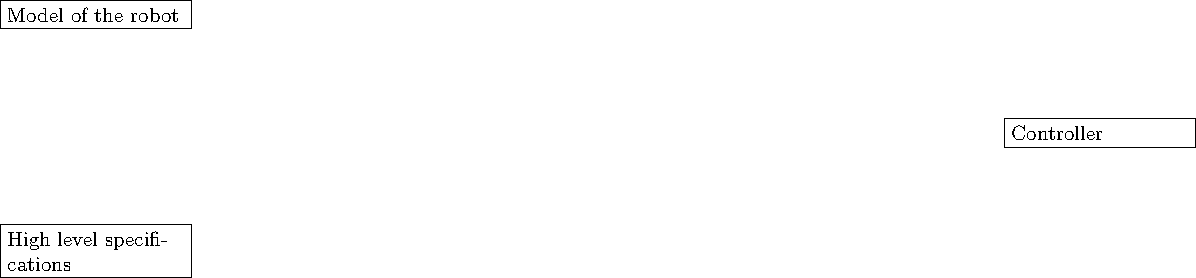
\includegraphics[width=\linewidth]{diagram.tex}
\label{diagram}
\end{figure}

Experiments on single agent, on 1 axis, 2 axis and on multi agents has been done when we managed to find a plan for the model.
The double integrator abstraction (without input memory) leads to abstractions that are unusable in 2D, as the input extended state abstraction with 1 input memory cannot be used with multi agent planning due to size of the abstraction.

\section{Single axis experiments}
We have been doing the synthesis of controller using different reduction of the second integrator model, we will compare the results to the raw second integrator model.
As we have seen in the previous parts, there is no need to test different values than the $\Delta n_u = 0$ and $\Delta n_u = 1$.
The case $\Delta n_u = 0$ (mode without any memories) correspond to the case of the single integrator.

\comment{Things to explains:
\begin{itemize}
\item How to choose the sampling time
\item How to configure the model
\item Speed profiles (add the velocity commands)
\item Computation of the time
\end{itemize}
}

For each of the models, the solution plans has been generated so that they have the less state as possible.


\subsection{Second integrator model with velocity feedback}
\begin{figure}[!ht]
	\begin{minipage}[b]{0.5\textwidth}
  		\centering
  		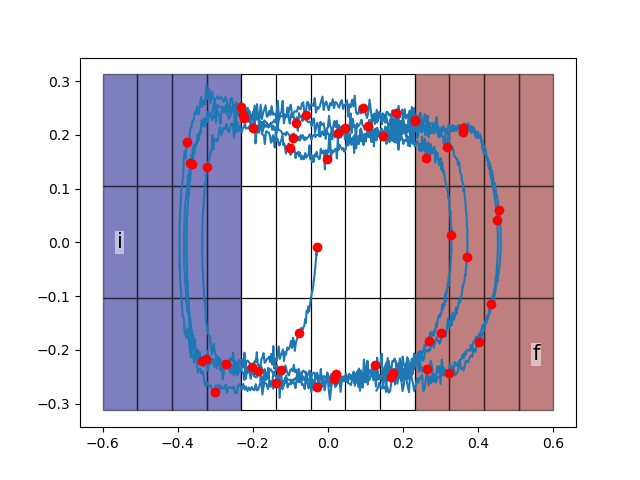
\includegraphics[width=0.9\linewidth]{double_1D}
	  	\caption{Trajectory in the 2D environment.}
	  	\label{double_1D}
  \end{minipage}
	\begin{minipage}[b]{0.5\textwidth}
  		\centering
  		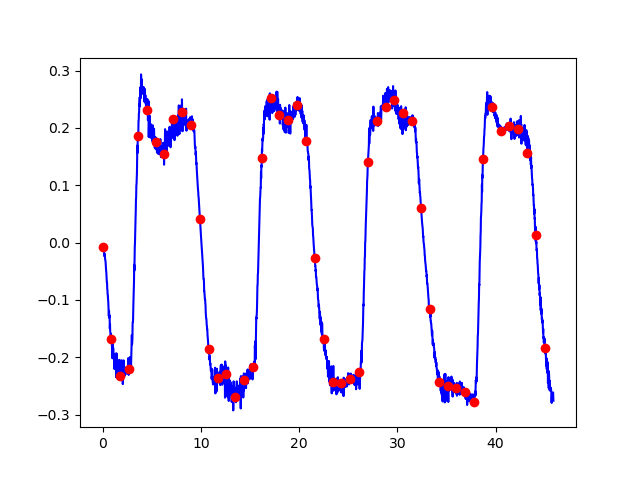
\includegraphics[width=0.9\linewidth]{double_1D_vel}
	  	\caption{Velocity profile.}
	  	\label{double_1D_vel}
  \end{minipage}
  \caption{Trajectory and velocity profile of the double integrator model. The agent is trying to achieve 'go infinity often to i and f'.}
\end{figure}

The model used is the "raw" second integrator model with velocity feedback.

%% SELF LOOPS ON THE VELOCITY AXIS
When creating the abstraction for such a model, the self loops are acceptable only for some controls and cell combinations. 
If the velocity of the quad is positive and the reference velocity negative, any self loop on the velocity axis will "keep" the next velocity state to the same cell.
This will create abstractions that are not controllable.
\comment{Do a graph about it}

\comment{plot the noise}

The second integrator model manage to take in account the transient state that was hidden by the single integrator model: in $x\approx0.4$, the transient states is clearly going "backward", this show that this model is not usable with the single integrator model (which correspond to non reachability behaviours).

\subsection{Model with $\Ninputs= 1$ memory}
\begin{figure}[!ht]
	\begin{minipage}[b]{0.5\textwidth}
  		\centering
  		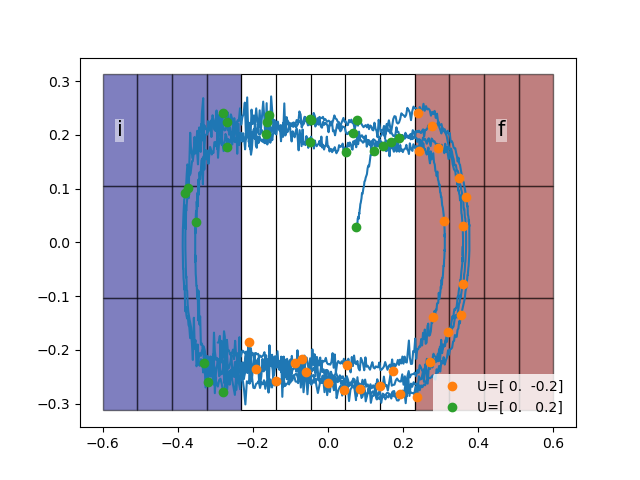
\includegraphics[width=\linewidth]{double_reduced_1D}
	  	\label{double_reduced_1D}
  \end{minipage}
	\begin{minipage}[b]{0.5\textwidth}
  		\centering
  		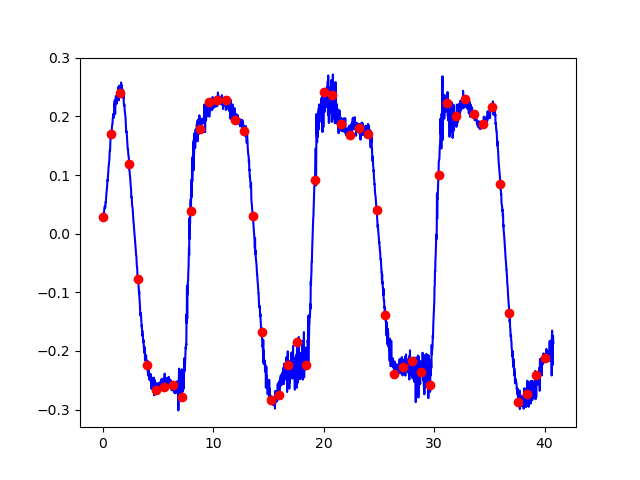
\includegraphics[width=\linewidth]{double_reduced_1D_vel}
	  	\label{double_reduced_1D_vel}
  \end{minipage}
  \caption{Trajectory and velocity profile of the double integrator reduced model. The agent is trying to achieve 'go infinity often to i and f'.}
\end{figure}

In our setup, the sampling time of model is ${\Delta t = 1s}$ and the timing constants of the reduced system is $\tau_r = {\nicefrac{1}{k} = 0.7s}$. This make relevant to use this reduction method as the internal dynamic of the quadricopter are not vanished enough after a $\Delta t$.


\subsection{Model with $\Ninputs= 1$ memory} \label{sec:single_int}
\begin{figure}[!ht]
	\begin{minipage}[b]{0.5\textwidth}
  		\centering
  		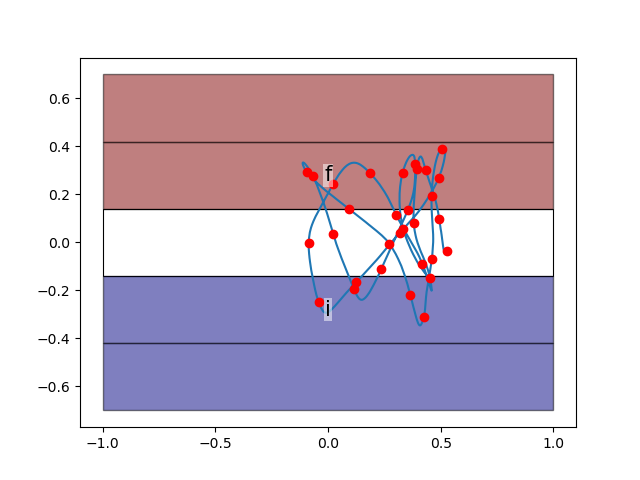
\includegraphics[width=0.9\linewidth]{simple_1D}
	  	\label{simple_1D}
  \end{minipage}
	\begin{minipage}[b]{0.5\textwidth}
  		\centering
  		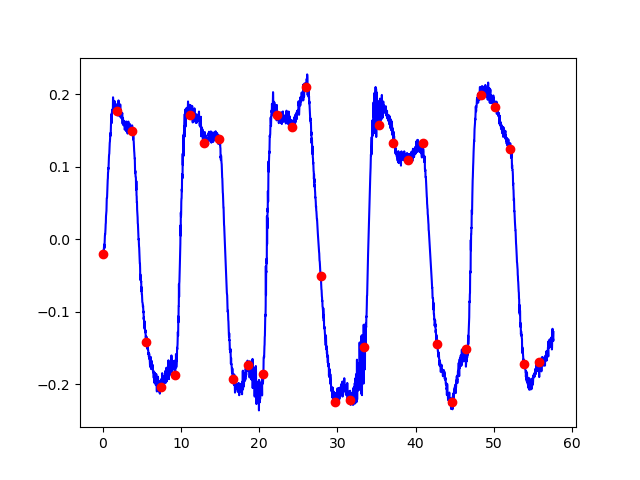
\includegraphics[width=0.9\linewidth]{simple_1D_vel}
	  	\label{simple_1D_vel}
  \end{minipage}
  \caption{Trajectory and velocity profile of the simple integrator model with self loops. The agent is trying to achieve 'go infinity often to i and f'.}
\end{figure}

\begin{figure}[!ht]
	\begin{minipage}[b]{0.5\textwidth}
  		\centering
  		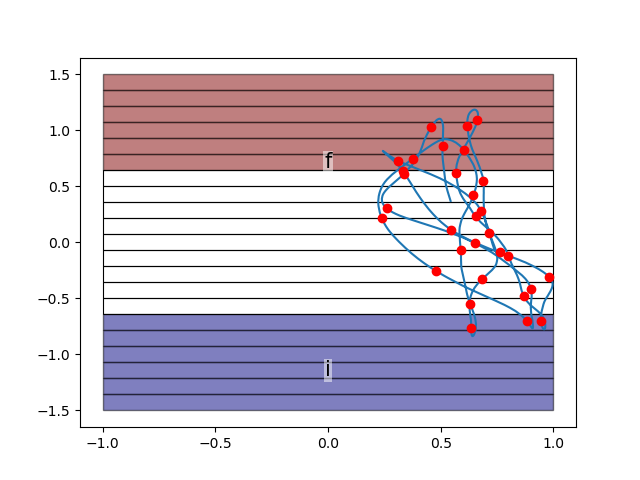
\includegraphics[width=0.9\linewidth]{simplenosl_1D}
	  	\label{simplenosl_1D}
  \end{minipage}
	\begin{minipage}[b]{0.5\textwidth}
  		\centering
  		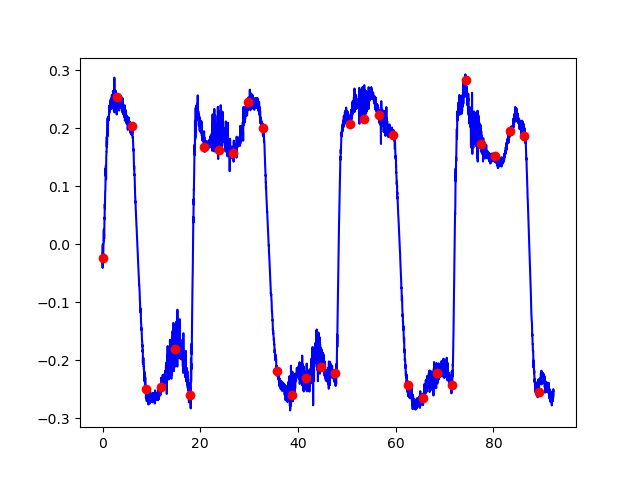
\includegraphics[width=0.9\linewidth]{simplenosl_1D_vel}
	  	\label{simplenosl_1D_vel}
  \end{minipage}
  \caption{Trajectory and velocity profile of the simple integrator model without self loops. The agent is trying to achieve 'go infinity often to i and f'.}
\end{figure}

\comment{Show the generated plans!}

This model is equivalent to the single integrator model.
We have been illustrating the advantages of self loops by doing one experiment with self loops and another experiment without self loops.
The FTS created without self loops needs to have a much finer discretization of the state space.
Whereas in the FTS with self loops the constraint on the minimal size of the state space discretization is only that the transient state on the velocity must counteract the effect of the noise.

\newcommand{\reg}[1]{\textit{reg #1}}
Other constraints apply on the sampling time: regions \reg{i} and \reg{f} needs to be reachable. If the sampling time is too high, the state might miss the target region.

When using a sampling time close to the transient time of the system, the reduction needs to take in account more states that belong to the transient states. This result in an increase of the modelled noise in the first integrator model.

\subsection{Comparison of the two results}
\begin{itemize}
\item compute the minimal number of states so that the model is usable (ie controllable)
\item compute the branching factor, the precision etc...
\item compute the amplitude of the noise in permanent state
\end{itemize}

Try to do it for different $\Delta n_u$, show that it does decrease the complexity for $\Delta n_u = 1$. Talk about the case $\Delta n_u = 0$ which correspond to the single integrator case (see part \ref{sec:single_int}).

Comparison to the double integrator case, show how the noise is evolving. Compare the size of the successors between the case where the discretization of the reduced state (velocity in this case) is lower than the steady state of the reduced state for a stable sequence. Basically, in one case, the size of the successors is growing (expansion of the successors) in the reduced approach, the size of the successors is reducing (but is bigger than the other one).


\comment{Try to show the 2 abstractions on top of each other to visualize what happened after the reduction}.

\paragraph{Sensitivity to noise}:
Please note that this model is less sensible to the noise on velocity as only the position is observed.
We have been noticing that this model was much easier to use thanks to this property.

\subsection{Experiments over 2 axes}

The previous study show the link between the precision and the complexity of the abstraction that we used.
In this part we will use the previous results in order to solve the following problem for different size of the environment:

\begin{figure}
	\center
	\includestandalone[width=0.5\textwidth]{2D_env_problem}
	\caption{Testing environment for the quadricopter.}
	\label{fig:environment}
\end{figure}

\comment{Show the simulation, the runs and so on.}


\subsection{Real case scenarios}

\begin{figure}[!ht]
  \centering
  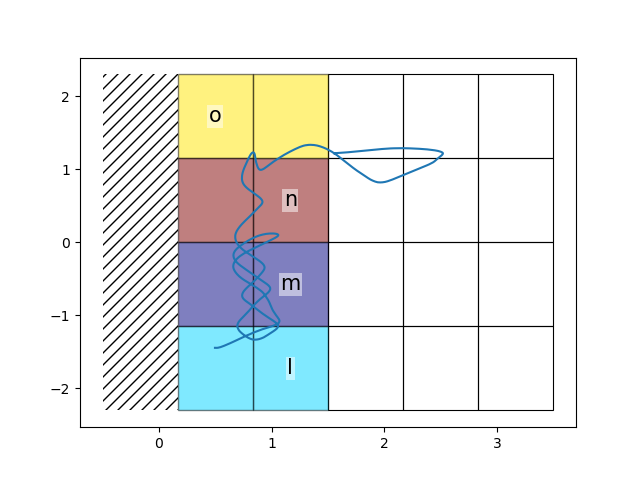
\includegraphics[width=0.9\linewidth]{real_case_scenarios}
  \caption{A trajectory in the state space $(x,v)$.}
\end{figure}

We have been using the first integrator model in this case (this is the more relevant in the scenario of the wind power).

\subsection{Discussion over the different models}
See table \ref{comparaison_table}.

\paragraph{Method:}
the comparison the different abstractions does not make any sense.
For example, in the second integrator abstraction, the discretization of the state space can be chosen to be the same than the reduced model, but we can always increase the precision over the velocity state.
We need to find a method that does not depend on a wrong parametrization of the method. Maybe defined the way we have been choosing the different abstraction (optimization criteria)?
So we need to use a standardized method in order to compare them.
For example, the minimum controllable abstraction might be a good choice.

There is no better abstraction, so we need to play with the parameters to show in which case the reduction is better than the original model.


\section{Experiments over 2 axes}
The previous study show the link between the precision and the complexity of the abstraction that we used.
In this part we will use the previous results in order to solve the following problem for different size of the environment.
\begin{figure}
	\center
	\includestandalone[width=0.5\textwidth]{2D_env_problem}
	\caption{Testing environment for the quadricopter.}
	\label{fig:environment}
\end{figure}

\comment{Show the simulation, the runs and so on.}

\subsection{$\Ninputs = 1$ input memory model}
See figure \ref{fig:double_reduce_2D}.

\begin{figure*}
	\center
	\includestandalone[width=\textwidth]{double_reduced_2D}
	\caption{$\Ninputs=1$ input memory model in 2D.}
	\label{fig:double_reduce_2D}
\end{figure*}

\subsection{$\Ninputs = 0$ input memory model}
See figure \ref{fig:double_reduce_2D}.


\subsection{Real case scenarios}
See figure \ref{fig:real_case}.
In the case of the wind turbine application, the quad will have to go from the base station to the wind turbine blade and explore a given set of regions while avoiding the blade.
The wind can be modelled as a perturbation on the velocity of the quadricopters.
We have been using the first integrator model in this case.

\begin{figure}[!ht]
  \centering
  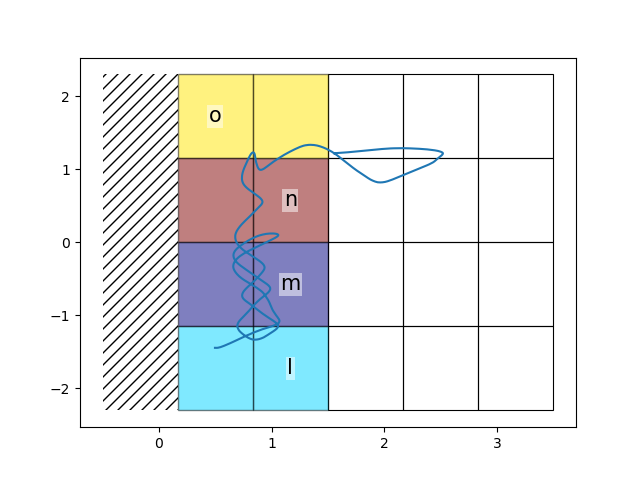
\includegraphics[width=0.9\linewidth]{real_case_scenarios}
  \caption{A trajectory in the state space $(x,v)$.}
  \label{fig:real_case}
\end{figure}


\section{Multi agent experiments}
The complexity of the problem disallow us from using a more complex model (double integrator, 1 input memory model) for multi agent scenarios.
Therefore, the $N$ quadricopters will be modelled as a $2N$ dimensions single integrators.

The quadricopters have to verify the following LTL formula:
$$ \varphi = (\LTLalways \neg out) \and (\LTLalways \LTLeventually a) \and (\LTLalways \LTLeventually b) \and (\LTLalways \neg collide)$$
where $out$ correspond to one quad or more outside of the environment, $a$ agent 1 in north-east and agent 2 in south-west, $b$ agent 1 in south-west and agent 2 in north-east and $collide$ if there is a collision (quads on the same cells).
Figure \ref{fig:multi} show a run of the plan for few steps.

\begin{figure}
  \newcommand*\FigVSkip{0.5em}
  \newcommand*\FigHSkip{0.1em}
  \newsavebox\FigBox
  \centering
  % Top image is centered, so no need to get width
  \begin{minipage}{0.3\textwidth}
    \centering
    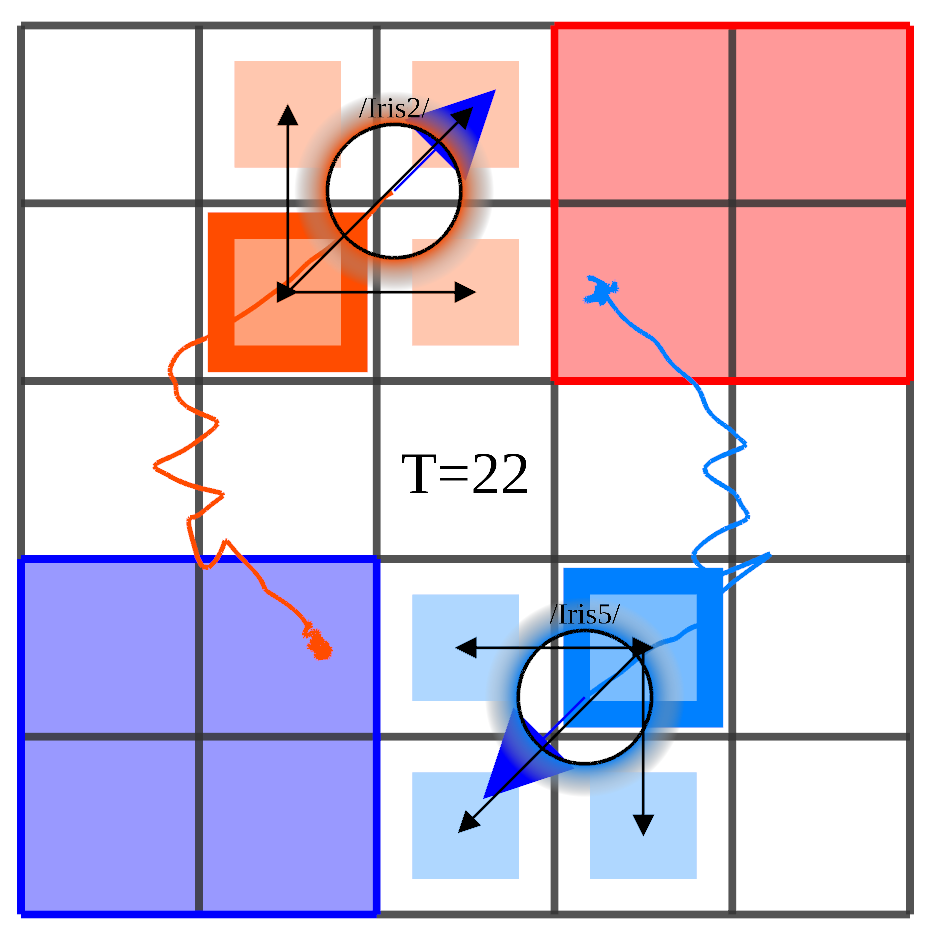
\includegraphics[width=\linewidth]{multi_ltl/multi1}
  \end{minipage} 
  \begin{minipage}{0.3\textwidth}
    \centering
    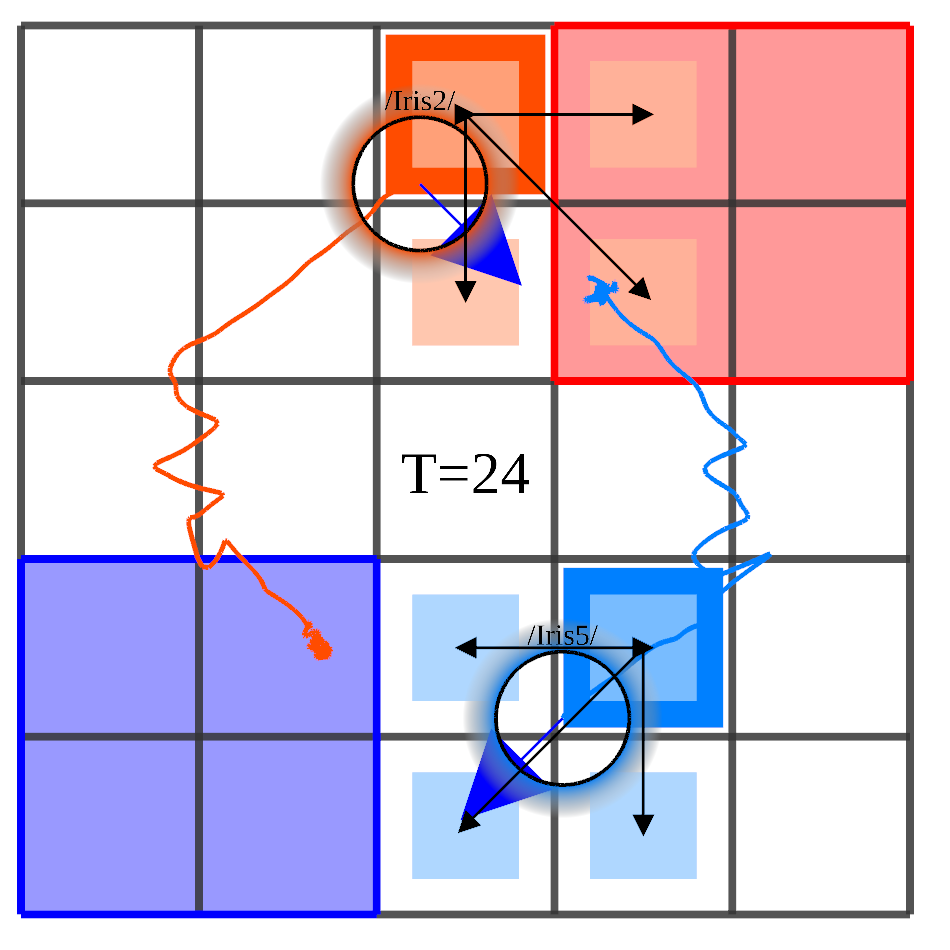
\includegraphics[width=\linewidth]{multi_ltl/multi2}
  \end{minipage} 
  \begin{minipage}{0.3\textwidth}
    \centering
    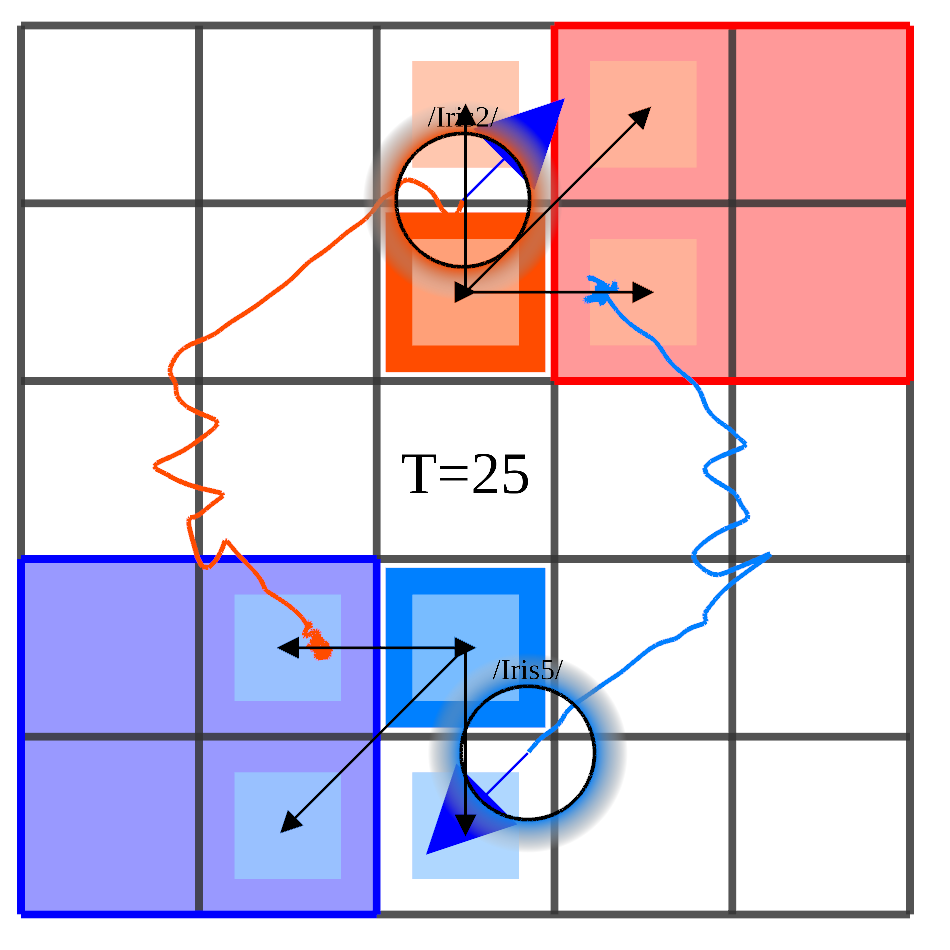
\includegraphics[width=\linewidth]{multi_ltl/multi3}
  \end{minipage} 
  \\[\FigVSkip]%
  % Top image is centered, so no need to get width
  \begin{minipage}{0.3\textwidth}
    \centering
    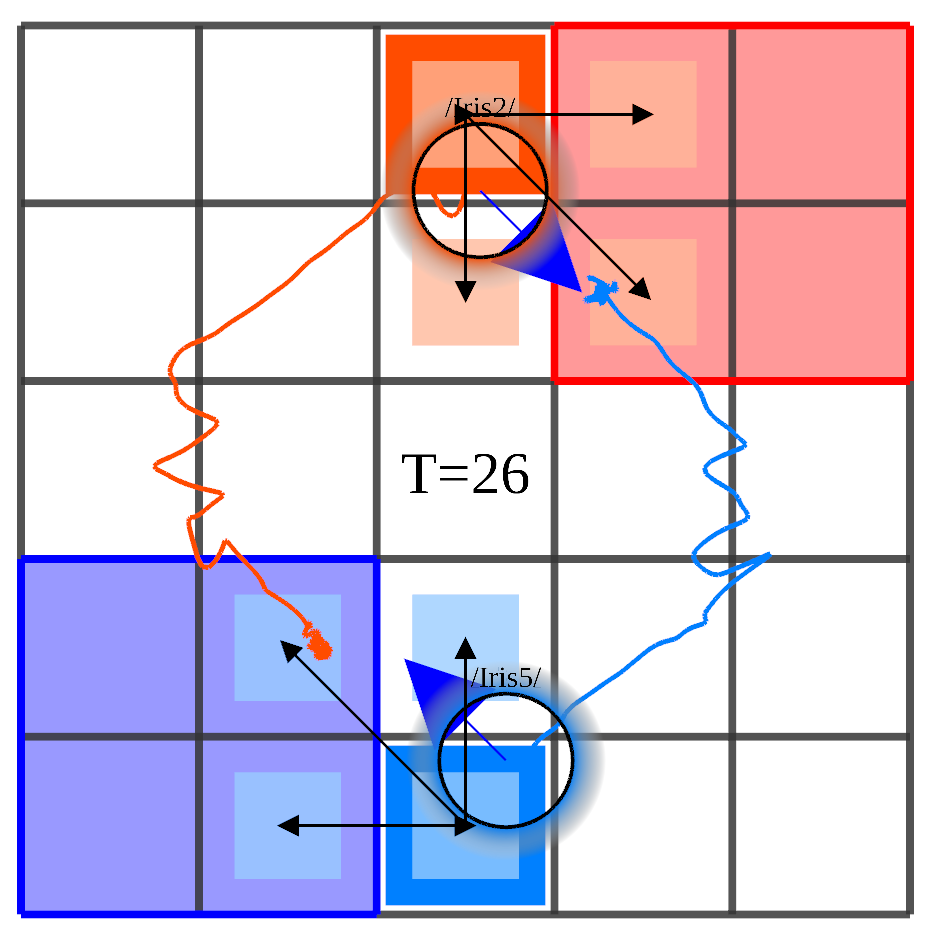
\includegraphics[width=\linewidth]{multi_ltl/multi4}
  \end{minipage} 
  \begin{minipage}{0.3\textwidth}
    \centering
    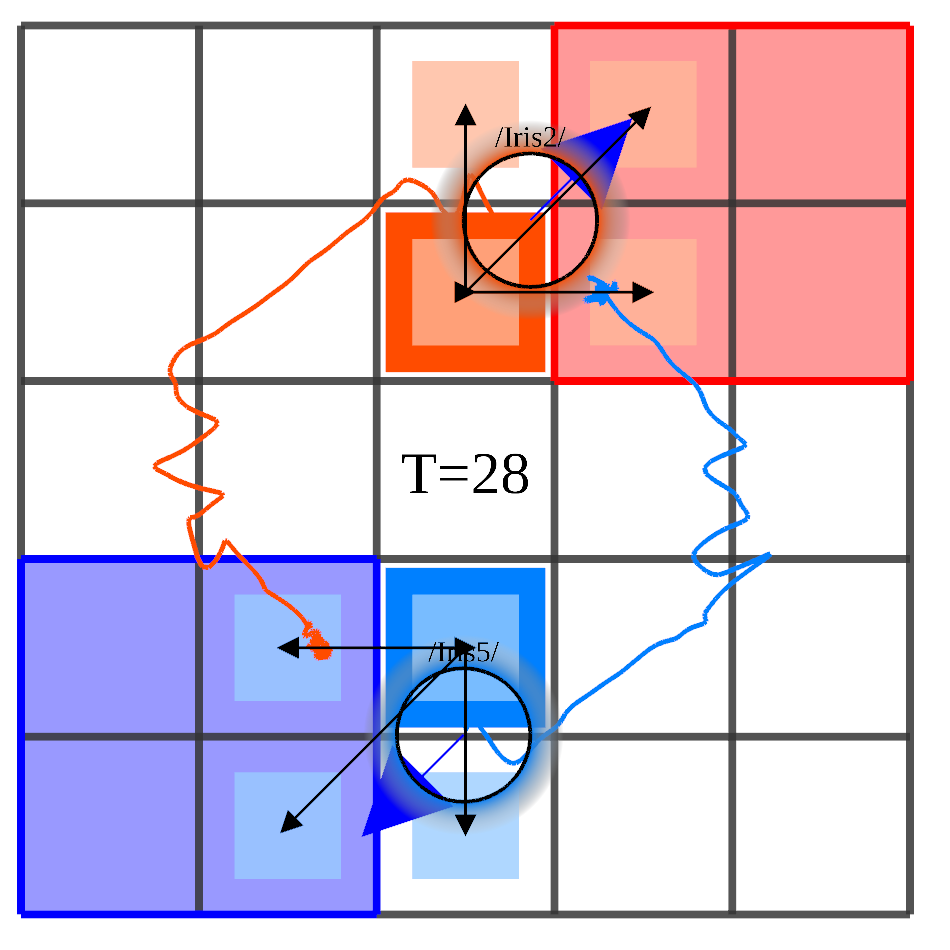
\includegraphics[width=\linewidth]{multi_ltl/multi5}
  \end{minipage} 
  \begin{minipage}{0.3\textwidth}
    \centering
    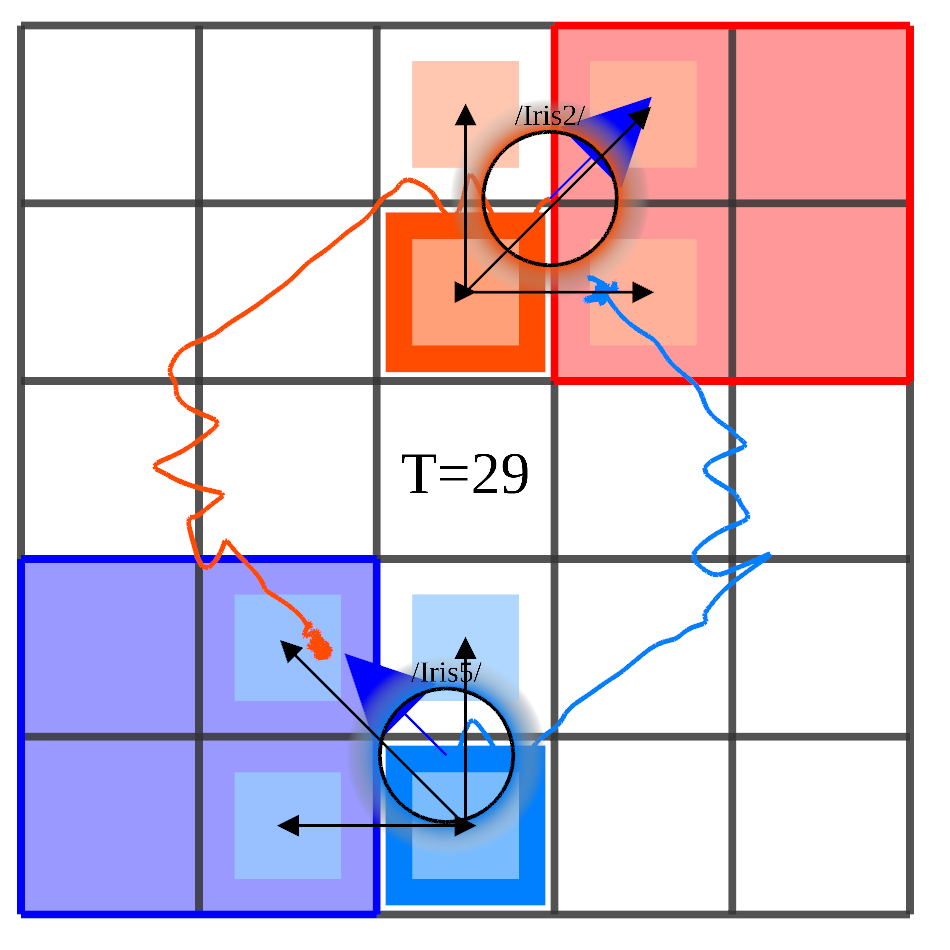
\includegraphics[width=\linewidth]{multi_ltl/multi6}
  \end{minipage} 
  \\[\FigVSkip]%
  % Top image is centered, so no need to get width
  \begin{minipage}{0.3\textwidth}
    \centering
    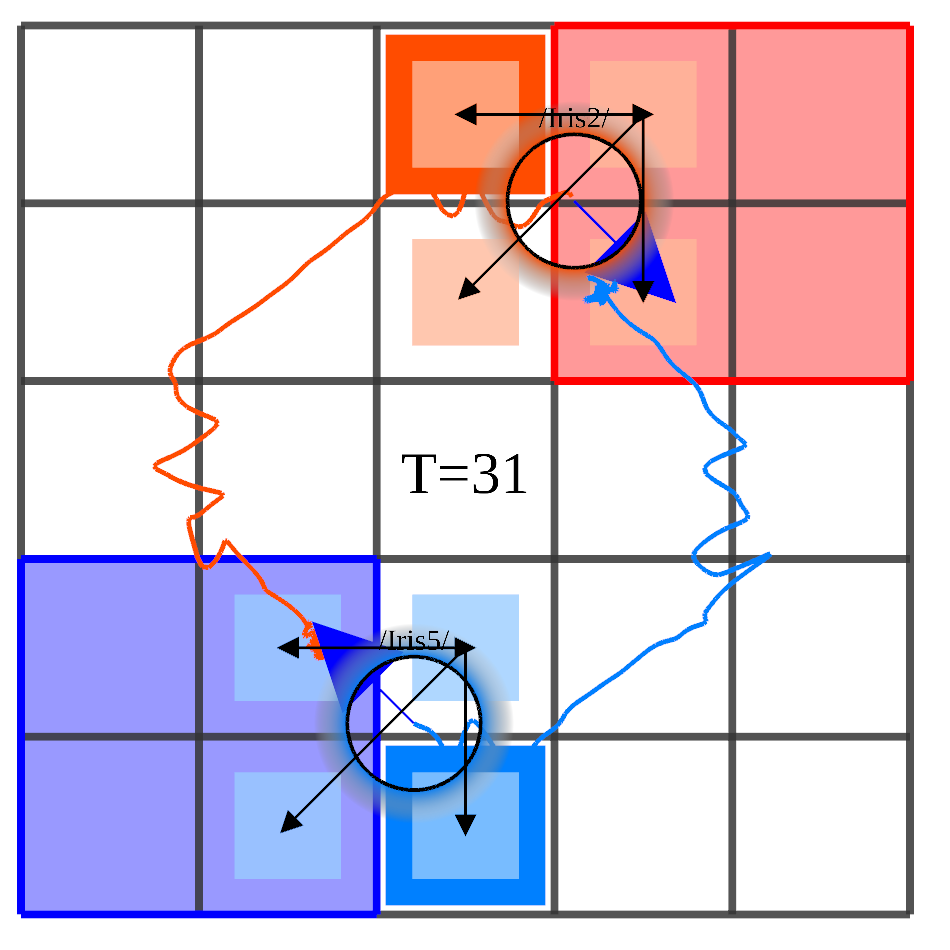
\includegraphics[width=\linewidth]{multi_ltl/multi7}
  \end{minipage} 
  \begin{minipage}{0.3\textwidth}
    \centering
    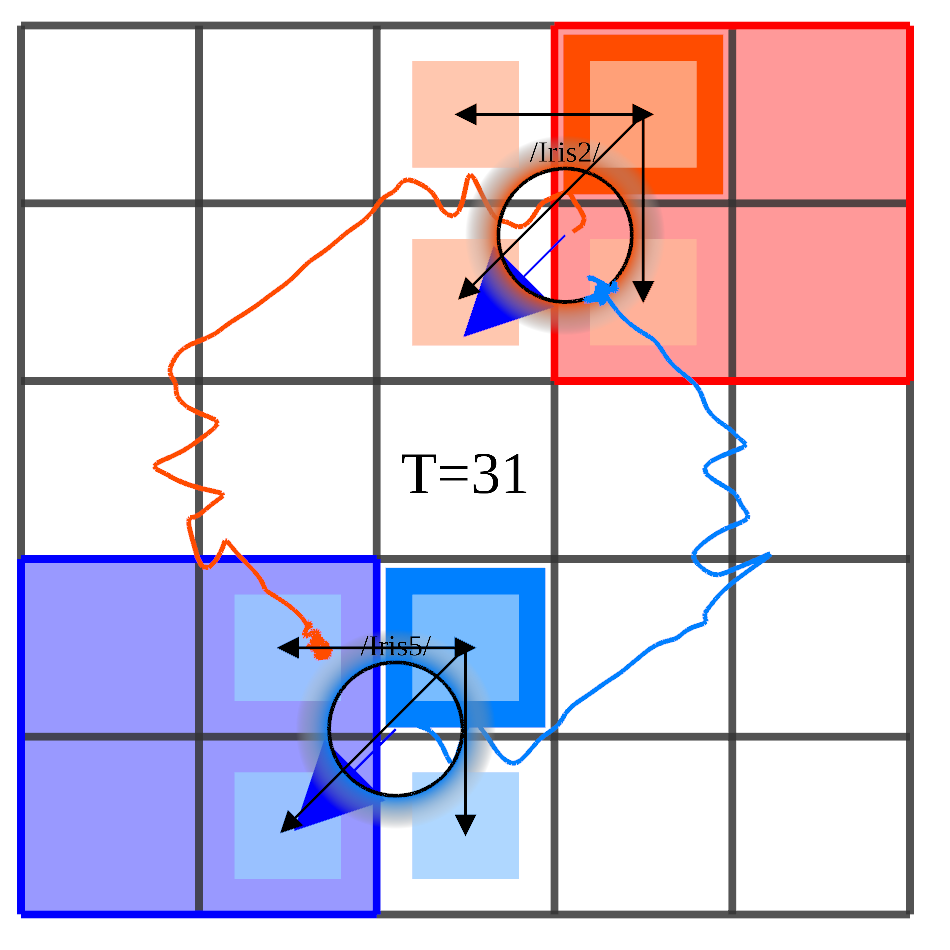
\includegraphics[width=\linewidth]{multi_ltl/multi8}
  \end{minipage} 
  \begin{minipage}{0.3\textwidth}
    \centering
    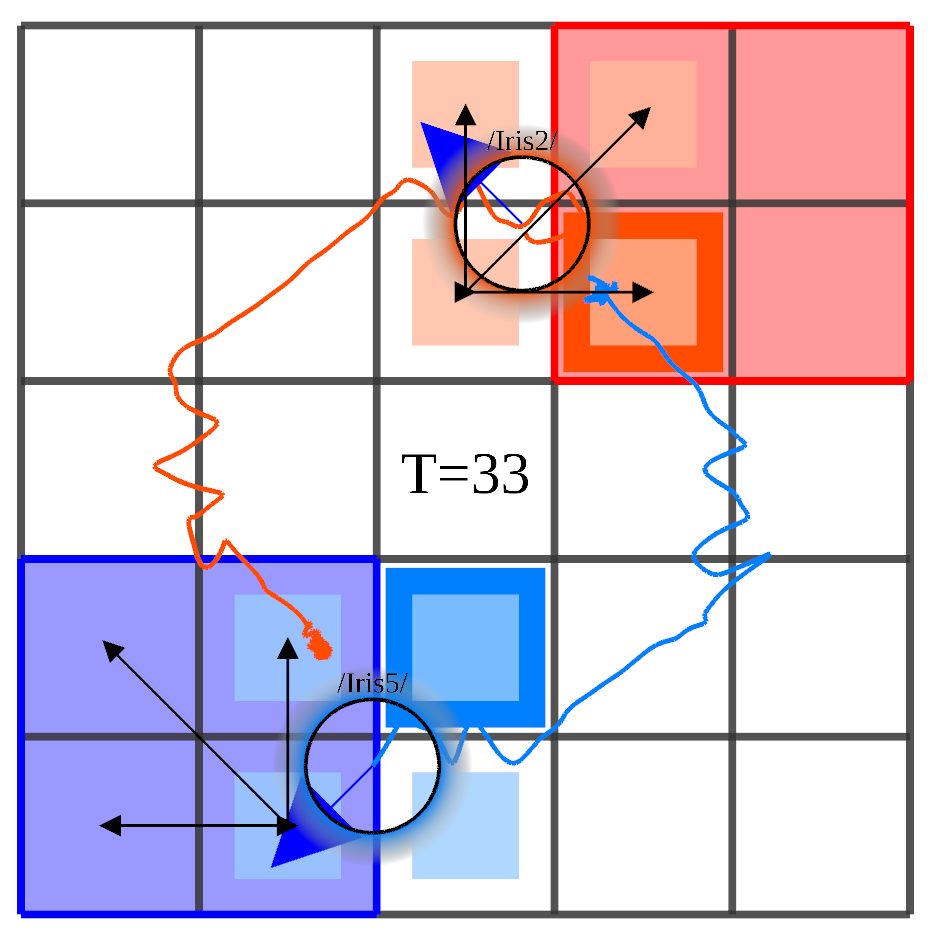
\includegraphics[width=\linewidth]{multi_ltl/multi9}
  \end{minipage} 
  \\[\FigVSkip]%
  % Top image is centered, so no need to get width
  \begin{minipage}{0.3\textwidth}
    \centering
    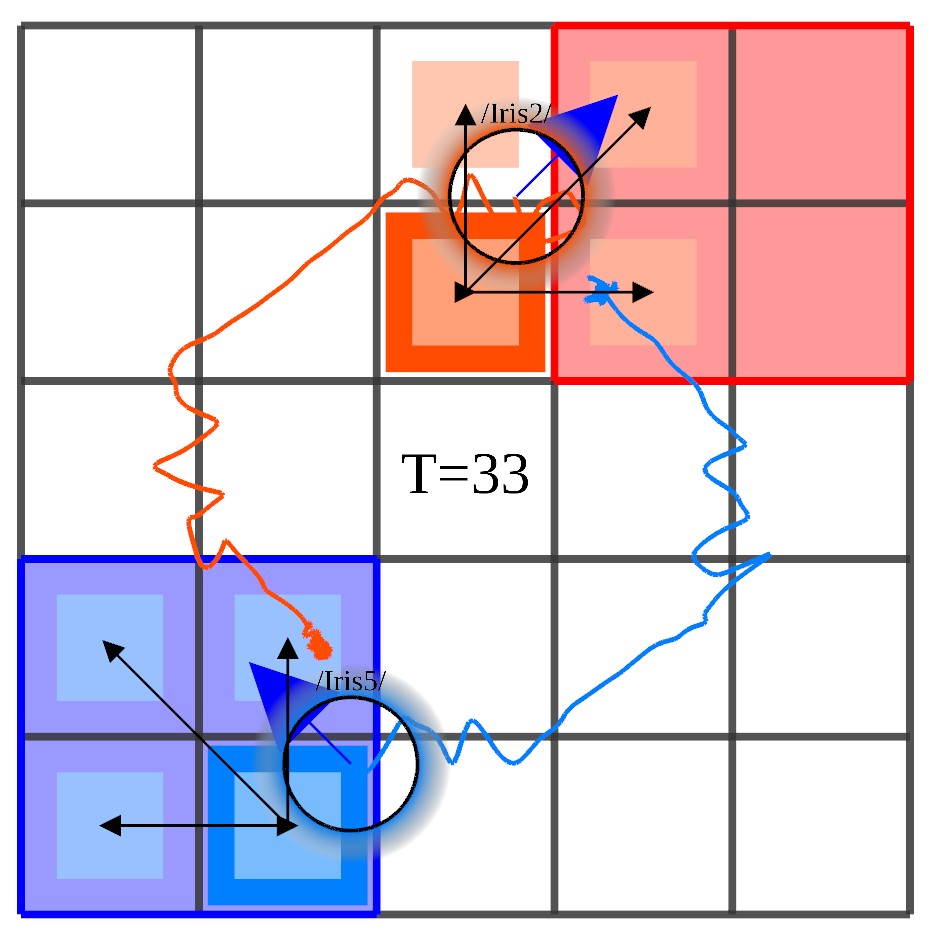
\includegraphics[width=\linewidth]{multi_ltl/multi10}
  \end{minipage} 
  \begin{minipage}{0.3\textwidth}
    \centering
    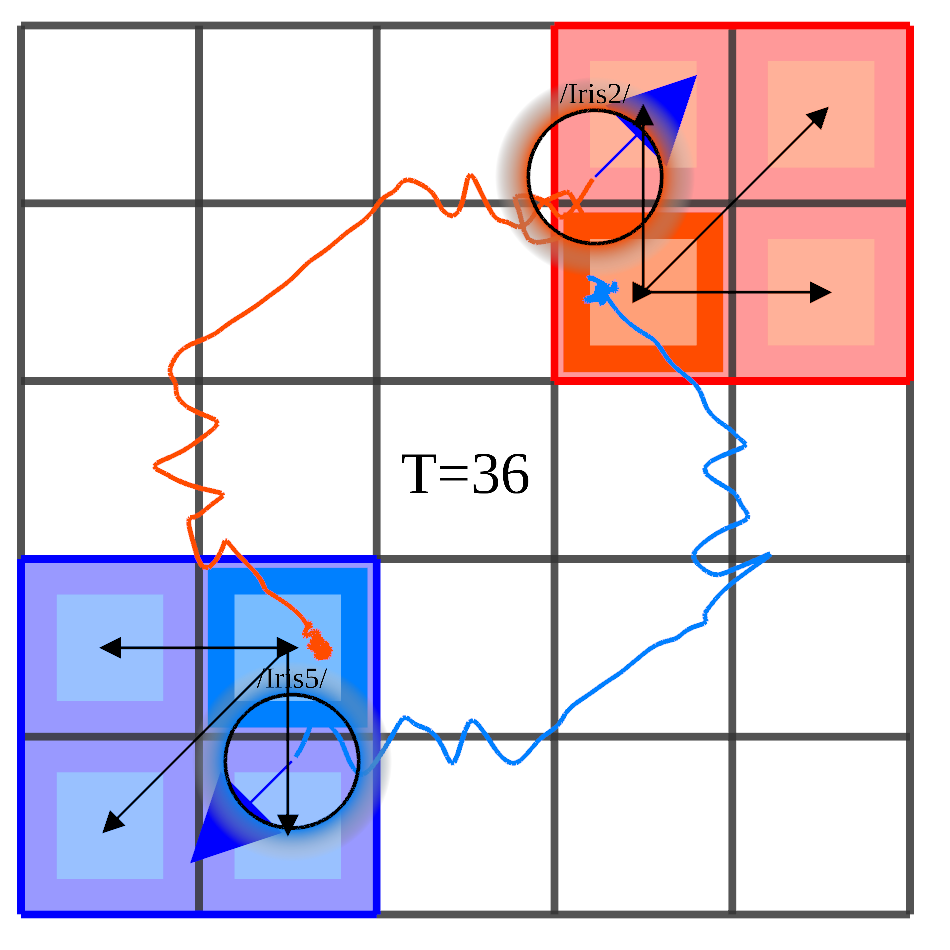
\includegraphics[width=\linewidth]{multi_ltl/multi11}
  \end{minipage} 
  \begin{minipage}{0.3\textwidth}
    \centering
    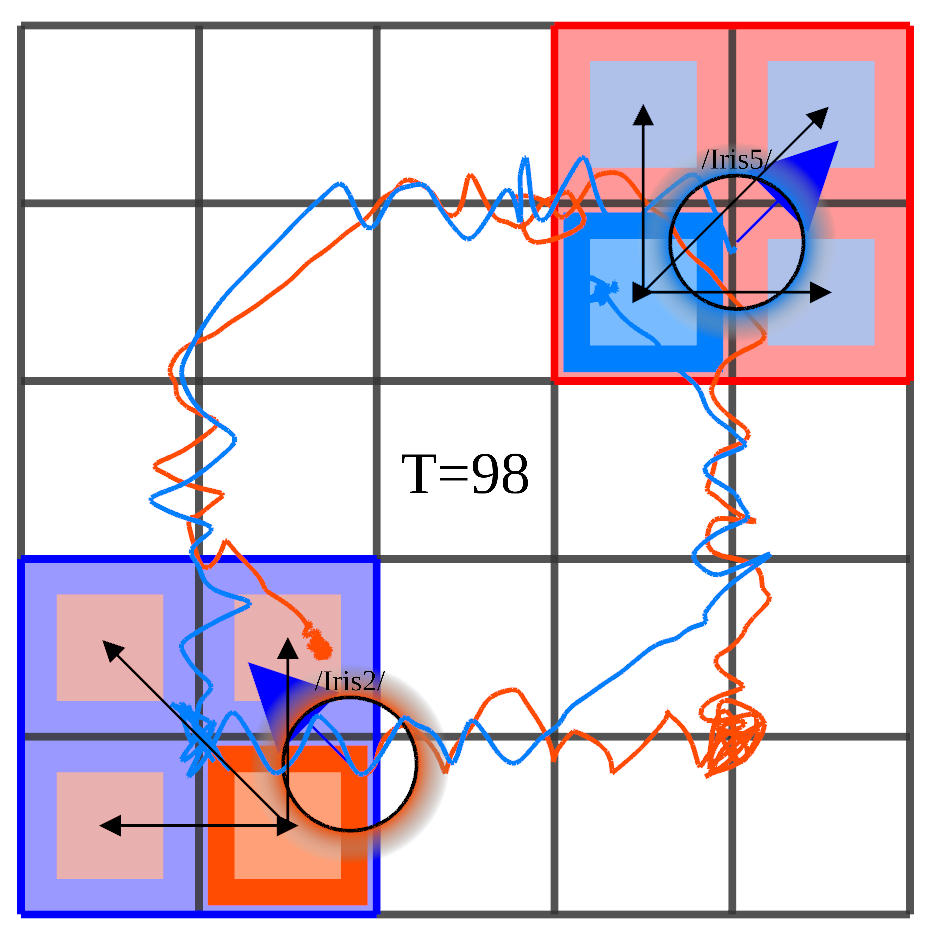
\includegraphics[width=\linewidth]{multi_ltl/multi12}
  \end{minipage} 

\caption{Run of the multiagent plan. Agent blue and red need to exchange position infinitely often. Cells in plain colors are the current state of the quadricopter. Cells in light color are the successors. Big blues arrows are the control action.}
\label{fig:multi}
\end{figure}


\section{Conclusion}
\comment{The strong cyclic planning method can be really effective in some case where the magnitude of the noise is higher than the control action (creating a possibility of leaving the cells).
Conclude about when to use the strongly connected cyclic model.
How to choose the discretization.
Just accept the fact that there is no strong theoretical justifications?
Can I sort of generalize this method to a bigger class of model (not just the first integrator model)?
}
\comment{I must notice that the we are not using any optimal algorithm (DFS). This imply that the computing time are less than a relevant case scenario.}


%\bibliographystyle{kthplain}
%\bibliography{bibliography}{}

\end{document}